\documentclass{article}\usepackage[]{graphicx}\usepackage[]{color}
%% maxwidth is the original width if it is less than linewidth
%% otherwise use linewidth (to make sure the graphics do not exceed the margin)
\makeatletter
\def\maxwidth{ %
  \ifdim\Gin@nat@width>\linewidth
    \linewidth
  \else
    \Gin@nat@width
  \fi
}
\makeatother

\definecolor{fgcolor}{rgb}{0.345, 0.345, 0.345}
\newcommand{\hlnum}[1]{\textcolor[rgb]{0.686,0.059,0.569}{#1}}%
\newcommand{\hlstr}[1]{\textcolor[rgb]{0.192,0.494,0.8}{#1}}%
\newcommand{\hlcom}[1]{\textcolor[rgb]{0.678,0.584,0.686}{\textit{#1}}}%
\newcommand{\hlopt}[1]{\textcolor[rgb]{0,0,0}{#1}}%
\newcommand{\hlstd}[1]{\textcolor[rgb]{0.345,0.345,0.345}{#1}}%
\newcommand{\hlkwa}[1]{\textcolor[rgb]{0.161,0.373,0.58}{\textbf{#1}}}%
\newcommand{\hlkwb}[1]{\textcolor[rgb]{0.69,0.353,0.396}{#1}}%
\newcommand{\hlkwc}[1]{\textcolor[rgb]{0.333,0.667,0.333}{#1}}%
\newcommand{\hlkwd}[1]{\textcolor[rgb]{0.737,0.353,0.396}{\textbf{#1}}}%

\usepackage{framed}
\makeatletter
\newenvironment{kframe}{%
 \def\at@end@of@kframe{}%
 \ifinner\ifhmode%
  \def\at@end@of@kframe{\end{minipage}}%
  \begin{minipage}{\columnwidth}%
 \fi\fi%
 \def\FrameCommand##1{\hskip\@totalleftmargin \hskip-\fboxsep
 \colorbox{shadecolor}{##1}\hskip-\fboxsep
     % There is no \\@totalrightmargin, so:
     \hskip-\linewidth \hskip-\@totalleftmargin \hskip\columnwidth}%
 \MakeFramed {\advance\hsize-\width
   \@totalleftmargin\z@ \linewidth\hsize
   \@setminipage}}%
 {\par\unskip\endMakeFramed%
 \at@end@of@kframe}
\makeatother

\definecolor{shadecolor}{rgb}{.97, .97, .97}
\definecolor{messagecolor}{rgb}{0, 0, 0}
\definecolor{warningcolor}{rgb}{1, 0, 1}
\definecolor{errorcolor}{rgb}{1, 0, 0}
\newenvironment{knitrout}{}{} % an empty environment to be redefined in TeX

\usepackage{alltt}
\usepackage{geometry}
\usepackage{amsmath}
\usepackage{lscape}
\geometry{verbose,tmargin=2.5cm,bmargin=2.5cm,lmargin=2.5cm,rmargin=2.5cm}
\IfFileExists{upquote.sty}{\usepackage{upquote}}{}
\begin{document}



\title{NSWPCN Predictor Training}
\maketitle

%%%%%%%%%%%%%%%%%%%%%%%%%%%%%%%%%%%%%%%%%%%%%%%%%%%%%%%%%%%%%%%%%%%%%%
% LIBRARIES
%%%%%%%%%%%%%%%%%%%%%%%%%%%%%%%%%%%%%%%%%%%%%%%%%%%%%%%%%%%%%%%%%%%%%%
\section{Preparation}
\begin{knitrout}
\definecolor{shadecolor}{rgb}{0.969, 0.969, 0.969}\color{fgcolor}\begin{kframe}
\begin{alltt}
\hlkwd{library}\hlstd{(survival)}
\end{alltt}


{\ttfamily\noindent\itshape\color{messagecolor}{\#\# Loading required package: splines}}\begin{alltt}
\hlkwd{library}\hlstd{(glmulti)}
\end{alltt}


{\ttfamily\noindent\itshape\color{messagecolor}{\#\# Loading required package: rJava\\\#\# Loading required package: methods}}\begin{alltt}
\hlkwd{library}\hlstd{(flexsurv)}
\hlkwd{library}\hlstd{(randomForestSRC)}
\end{alltt}


{\ttfamily\noindent\itshape\color{messagecolor}{\#\# Loading required package: parallel\\\#\# \\\#\#\ \ randomForestSRC 1.5.5 \\\#\#\ \ \\\#\#\ \ Type rfsrc.news() to see new features, changes, and bug fixes. \\\#\# }}\begin{alltt}
\hlkwd{library}\hlstd{(reshape2)}
\hlkwd{library}\hlstd{(plyr)}
\hlkwd{library}\hlstd{(ggplot2)}

\hlkwd{library}\hlstd{(MASS)}
\hlkwd{library}\hlstd{(boot)}
\end{alltt}


{\ttfamily\noindent\itshape\color{messagecolor}{\#\# \\\#\# Attaching package: 'boot'\\\#\# \\\#\# The following object is masked from 'package:survival':\\\#\# \\\#\#\ \ \ \  aml}}\begin{alltt}
\hlkwd{library}\hlstd{(timeROC)}
\end{alltt}


{\ttfamily\noindent\itshape\color{messagecolor}{\#\# Loading required package: pec\\\#\# Loading required package: mvtnorm\\\#\# Loading required package: timereg}}\begin{alltt}
\hlkwd{load}\hlstd{(}\hlstr{"03_NSWPCN_subset.rda"}\hlstd{)}

\hlkwd{library}\hlstd{(RColorBrewer)}
\hlstd{pal} \hlkwb{=} \hlkwd{brewer.pal}\hlstd{(}\hlnum{4}\hlstd{,} \hlstr{"Dark2"}\hlstd{)}
\hlkwd{names}\hlstd{(pal)} \hlkwb{=} \hlkwd{c}\hlstd{(}\hlstr{"GG"}\hlstd{,} \hlstr{"CPH"}\hlstd{,} \hlstr{"RSF"}\hlstd{,} \hlstr{"KM0"}\hlstd{)}
\end{alltt}
\end{kframe}
\end{knitrout}


%%%%%%%%%%%%%%%%%%%%%%%%%%%%%%%%%%%%%%%%%%%%%%%%%%%%%%%%%%%%%%%%%%%%%%
% DATA SELECTION
%%%%%%%%%%%%%%%%%%%%%%%%%%%%%%%%%%%%%%%%%%%%%%%%%%%%%%%%%%%%%%%%%%%%%%
\section{Cohort selection and transformation}
\begin{knitrout}
\definecolor{shadecolor}{rgb}{0.969, 0.969, 0.969}\color{fgcolor}\begin{kframe}
\begin{alltt}
\hlstd{data}\hlopt{$}\hlstd{SexM} \hlkwb{=} \hlstd{data}\hlopt{$}\hlstd{Patient.Sex} \hlopt{==} \hlstr{"M"}
\hlstd{data}\hlopt{$}\hlstd{Ca199} \hlkwb{=} \hlstd{data}\hlopt{$}\hlstd{Path.Ca199.Preop} \hlopt{>} \hlnum{100}
\hlstd{data}\hlopt{$}\hlstd{DiagYearCent} \hlkwb{=} \hlkwd{as.numeric}\hlstd{((data}\hlopt{$}\hlstd{History.Diagnosis.Date} \hlopt{-} \hlkwd{median}\hlstd{(data}\hlopt{$}\hlstd{History.Diagnosis.Date))} \hlopt{/} \hlnum{365.25}\hlstd{)}
\hlstd{data}\hlopt{$}\hlstd{Time} \hlkwb{=} \hlkwd{as.numeric}\hlstd{(data}\hlopt{$}\hlstd{History.Death.Date} \hlopt{-} \hlstd{data}\hlopt{$}\hlstd{History.Diagnosis.Date)}
\hlstd{data}\hlopt{$}\hlstd{DSD} \hlkwb{=} \hlstd{data}\hlopt{$}\hlstd{History.DSDeath.Event} \hlopt{==} \hlnum{1}
\hlstd{data}\hlopt{$}\hlstd{AgeCent} \hlkwb{=} \hlstd{data}\hlopt{$}\hlstd{History.Diagnosis.AgeAt.Cent}
\hlstd{data}\hlopt{$}\hlstd{LocBody} \hlkwb{=} \hlstd{data}\hlopt{$}\hlstd{Path.LocationBody}
\hlstd{data}\hlopt{$}\hlstd{SizeCent} \hlkwb{=} \hlstd{data}\hlopt{$}\hlstd{Path.Size.Cent}
\hlstd{data}\hlopt{$}\hlstd{A2} \hlkwb{=} \hlstd{data}\hlopt{$}\hlstd{Molec.S100A2.DCThresh}
\hlstd{data}\hlopt{$}\hlstd{A4} \hlkwb{=} \hlstd{data}\hlopt{$}\hlstd{Molec.S100A4.DCThresh}

\hlkwd{median}\hlstd{(data}\hlopt{$}\hlstd{DiagYearCent)}
\end{alltt}
\begin{verbatim}
## [1] 0
\end{verbatim}
\begin{alltt}
\hlkwd{hist}\hlstd{(data}\hlopt{$}\hlstd{DiagYearCent,} \hlkwc{main} \hlstd{=} \hlstr{"Histogram of Median-Centered Diagnosis Year"}\hlstd{,} \hlkwc{xlab} \hlstd{=} \hlstr{""}\hlstd{)}
\end{alltt}
\end{kframe}

{\centering 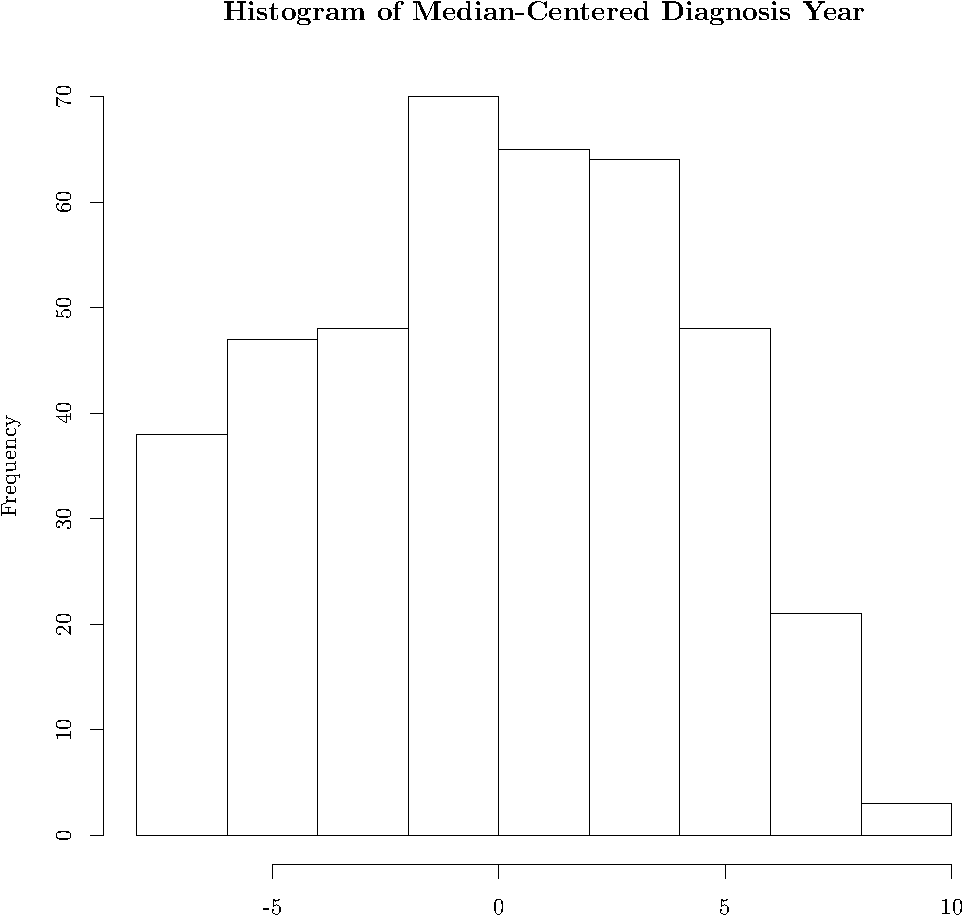
\includegraphics[width=\maxwidth]{figure/05-data-selection-1} 

}


\begin{kframe}\begin{alltt}
\hlstd{temp} \hlkwb{=} \hlnum{NA}
\hlstd{temp} \hlkwb{=} \hlkwd{ls}\hlstd{()}
\hlkwd{rm}\hlstd{(}\hlkwc{list} \hlstd{= temp[}\hlopt{!}\hlstd{(temp} \hlopt \hlkwd{c}\hlstd{(}\hlstr{"pal"}\hlstd{,} \hlstr{"data"}\hlstd{))])}

\hlkwd{nrow}\hlstd{(data)}
\end{alltt}
\begin{verbatim}
## [1] 404
\end{verbatim}
\begin{alltt}
\hlstd{data} \hlkwb{=} \hlstd{data[}\hlopt{!}\hlkwd{is.na}\hlstd{(data}\hlopt{$}\hlstd{Time)} \hlopt{& !}\hlkwd{is.na}\hlstd{(data}\hlopt{$}\hlstd{DSD)} \hlopt{& !}\hlkwd{is.na}\hlstd{(data}\hlopt{$}\hlstd{A2)} \hlopt{& !}\hlkwd{is.na}\hlstd{(data}\hlopt{$}\hlstd{A4)} \hlopt{& !}\hlkwd{is.na}\hlstd{(data}\hlopt{$}\hlstd{LocBody),]}
\hlkwd{nrow}\hlstd{(data)}
\end{alltt}
\begin{verbatim}
## [1] 256
\end{verbatim}
\begin{alltt}
\hlstd{data} \hlkwb{=} \hlstd{data[data}\hlopt{$}\hlstd{Time} \hlopt{<} \hlnum{3000}\hlstd{,]}          \hlcom{# Remove long-term survivors, which are very likely to be data errors}
\hlkwd{nrow}\hlstd{(data)}
\end{alltt}
\begin{verbatim}
## [1] 249
\end{verbatim}
\begin{alltt}
\hlstd{data.all} \hlkwb{=} \hlstd{data}
\hlkwd{nrow}\hlstd{(data.all)}
\end{alltt}
\begin{verbatim}
## [1] 249
\end{verbatim}
\begin{alltt}
\hlkwd{summary}\hlstd{(data.all)}
\end{alltt}
\begin{verbatim}
##    Patient.ID   Patient.Sex Cohort.ICGC     History.PreviousMalignancy
##  Min.   :   4   F:126       Mode :logical   Mode :logical             
##  1st Qu.: 305   M:123       FALSE:249       FALSE:227                 
##  Median : 638               NA's :0         TRUE :22                  
##  Mean   : 621                               NA's :0                   
##  3rd Qu.:1031                                                         
##  Max.   :1453                                                         
##                                                                       
##  History.FdrWithPancCancer History.FdrWithAnyCancer History.Diagnosis.Date
##  Mode :logical             Mode :logical            Min.   :1994-03-09    
##  FALSE:239                 FALSE:210                1st Qu.:1998-06-11    
##  TRUE :8                   TRUE :39                 Median :2001-07-28    
##  NA's :2                   NA's :0                  Mean   :2000-12-26    
##                                                     3rd Qu.:2003-06-26    
##                                                     Max.   :2006-08-14    
##                                                                           
##  History.Diagnosis.AgeAt History.AlcoholLevel History.Smoking.Status
##  Min.   :28.0            0:158                Never  :144           
##  1st Qu.:62.0            1: 46                Ceased : 51           
##  Median :69.0            2: 22                Current: 54           
##  Mean   :67.4            3: 23                                      
##  3rd Qu.:75.0                                                       
##  Max.   :87.0                                                       
##                                                                     
##  History.Smoking.PackYears History.Comorbid.Diabetes
##  Min.   : 2.0              Mode :logical            
##  1st Qu.:20.0              FALSE:186                
##  Median :27.5              TRUE :63                 
##  Mean   :31.6              NA's :0                  
##  3rd Qu.:46.2                                       
##  Max.   :80.0                                       
##  NA's   :189                                        
##  History.Comorbid.ChronicPancreatitis History.Recurrence.Event
##  Mode :logical                        Min.   :0.00            
##  FALSE:238                            1st Qu.:1.00            
##  TRUE :11                             Median :1.00            
##  NA's :0                              Mean   :0.96            
##                                       3rd Qu.:1.00            
##                                       Max.   :1.00            
##                                                               
##  History.Recurrence.Date History.DSDeath.Event History.Death.Date  
##  Min.   :1994-07-21      Min.   :0.000         Min.   :1995-01-12  
##  1st Qu.:2000-01-08      1st Qu.:1.000         1st Qu.:1999-12-01  
##  Median :2002-06-03      Median :1.000         Median :2002-12-18  
##  Mean   :2002-03-22      Mean   :0.952         Mean   :2002-09-02  
##  3rd Qu.:2005-02-04      3rd Qu.:1.000         3rd Qu.:2005-05-21  
##  Max.   :2009-01-29      Max.   :1.000         Max.   :2011-10-03  
##  NA's   :85                                                        
##  History.Followup.Date History.Death.EventTimeDays Treat.Resected
##  Min.   :2009-10-24    Min.   :  20                Mode:logical  
##  1st Qu.:2009-10-24    1st Qu.: 270                TRUE:249      
##  Median :2009-10-24    Median : 479                NA's:0        
##  Mean   :2009-11-30    Mean   : 617                              
##  3rd Qu.:2009-10-24    3rd Qu.: 851                              
##  Max.   :2010-06-03    Max.   :2701                              
##  NA's   :243                                                     
##  Treat.ProcedureWhipple Treat.MarginPositive Treat.Chemo.Any
##  Mode :logical          Mode :logical        Mode :logical  
##  FALSE:48               FALSE:145            FALSE:101      
##  TRUE :201              TRUE :104            TRUE :121      
##  NA's :0                NA's :0              NA's :27       
##                                                             
##                                                             
##                                                             
##  Treat.Chemo.Adjuvant Treat.Chemo.Adjuvant.GE3Cycles
##  Mode :logical        Mode :logical                 
##  FALSE:175            FALSE:204                     
##  TRUE :74             TRUE :45                      
##  NA's :0              NA's :0                       
##                                                     
##                                                     
##                                                     
##  Treat.Chemo.Palliative Treat.Chemo.PalliativeDC Treat.Chemo.GEM
##  Mode :logical          Mode :logical            Mode :logical  
##  FALSE:1                FALSE:178                FALSE:156      
##  TRUE :66               TRUE :71                 TRUE :92       
##  NA's :182              NA's :0                  NA's :1        
##                                                                 
##                                                                 
##                                                                 
##  Treat.Radio     Path.LocationBody   Path.Size    Path.Bilirubin.Preop
##  Mode :logical   Mode :logical     Min.   : 8.0   Min.   : 0.06       
##  FALSE:205       FALSE:201         1st Qu.:25.0   1st Qu.: 0.64       
##  TRUE :44        TRUE :48          Median :30.0   Median : 3.45       
##  NA's :0         NA's :0           Mean   :33.6   Mean   : 7.10       
##                                    3rd Qu.:40.0   3rd Qu.:10.22       
##                                    Max.   :90.0   Max.   :45.03       
##                                                   NA's   :99          
##  Path.Ca199.Preop Path.Bilirubin.Postop Path.Ca199.Postop
##  Min.   :     1   Min.   : 0.12         Min.   :    1    
##  1st Qu.:    67   1st Qu.: 0.47         1st Qu.:   15    
##  Median :   197   Median : 0.70         Median :   74    
##  Mean   :  2701   Mean   : 1.92         Mean   : 1528    
##  3rd Qu.:   802   3rd Qu.: 1.26         3rd Qu.:  271    
##  Max.   :101075   Max.   :25.38         Max.   :31760    
##  NA's   :168      NA's   :106           NA's   :143      
##         Path.Subtype Path.Differentiation Path.LN.Involved
##  Adenosquamous: 18   1: 16                Min.   : 0.00   
##  Large Cell   :  0   2:162                1st Qu.: 0.00   
##  Mucinous     :  5   3: 71                Median : 1.00   
##  NotSpecified : 39   4:  0                Mean   : 1.72   
##  Papillary    :  2                        3rd Qu.: 2.00   
##  Tubular      :185                        Max.   :12.00   
##                                           NA's   :4       
##  Path.LN.Inspected Path.Invasion.Vascular Path.Invasion.Perineural
##  Min.   : 0.0      Mode :logical          Mode :logical           
##  1st Qu.: 5.0      FALSE:133              FALSE:63                
##  Median : 8.5      TRUE :116              TRUE :186               
##  Mean   : 9.8      NA's :0                NA's :0                 
##  3rd Qu.:13.0                                                     
##  Max.   :52.0                                                     
##  NA's   :21                                                       
##  Stage.pT  Stage.pN   Stage.pM   Molec.BNIP3.NucInt Molec.BNIP3.CytoInt
##  Tis:  0   N0  : 83   M0  :182   0   :  6           0   :  1           
##  T1 : 18   N1  :160   M1  :  9   1   :208           1   :130           
##  T2 : 34   NA's:  6   NA's: 58   2   : 21           2   : 76           
##  T3 :197                         3   :  2           3   : 30           
##  T4 :  0                         NA's: 12           NA's: 12           
##                                                                        
##                                                                        
##  Molec.CCND1.CytoLo Molec.CCND1.CytoHi Molec.CCND1.MembLo
##  0   :159           0   :75            0   :100          
##  1   : 34           1   :90            1   : 71          
##  2   :  4           2   :32            2   : 18          
##  3   :  1           3   : 1            3   :  9          
##  NA's: 51           NA's:51            NA's: 51          
##                                                          
##                                                          
##  Molec.CCND1.MembHi Molec.Grb7.Int Molec.Grb7.Percent Molec.HCNT3PlusHENT1
##  0   :32            0   :51        Min.   :  0.0      Mode :logical       
##  1   :89            1   :94        1st Qu.:  3.0      FALSE:96            
##  2   :46            2   :42        Median : 18.0      TRUE :98            
##  3   :31            3   : 7        Mean   : 31.1      NA's :55            
##  NA's:51            NA's:55        3rd Qu.: 55.0                          
##                                    Max.   :100.0                          
##                                    NA's   :55                             
##  Molec.HENT1.Percent Molec.HENT1.Int Molec.HER2      Molec.HOXB2.Percent
##  Min.   :  0.0       0   : 19        Mode :logical   Min.   :  0.0      
##  1st Qu.: 11.2       1   :117        FALSE:37        1st Qu.: 35.0      
##  Median : 42.5       2   : 53        TRUE :11        Median : 70.0      
##  Mean   : 44.4       3   : 13        NA's :201       Mean   : 60.8      
##  3rd Qu.: 75.0       NA's: 47                        3rd Qu.: 90.0      
##  Max.   :100.0                                       Max.   :100.0      
##  NA's   :47                                          NA's   :43         
##  Molec.HOXB2.Int Molec.RON.Int Molec.S100A2.Int Molec.S100A2.Percent
##  0   : 14        0   : 20      0:88             Min.   :  0.0       
##  1   :141        1   :111      1:63             1st Qu.:  0.0       
##  2   : 36        2   : 64      2:57             Median : 10.0       
##  3   : 15        3   : 10      3:41             Mean   : 28.7       
##  NA's: 43        NA's: 44                       3rd Qu.: 60.0       
##                                                 Max.   :100.0       
##                                                                     
##  Molec.S100A2.StromaScore Molec.S100A4.CytoInt Molec.S100A4.CytoPercent
##  Mode :logical            0:72                 Min.   :  0.0           
##  FALSE:183                1:93                 1st Qu.:  0.0           
##  TRUE :22                 2:43                 Median : 10.0           
##  NA's :44                 3:41                 Mean   : 34.6           
##                                                3rd Qu.: 75.0           
##                                                Max.   :100.0           
##                                                                        
##  Molec.S100A4.NucInt Molec.S100A4.NucPercent Stage.Overall
##  0:80                Min.   :  0.0           IIB    :120  
##  1:68                1st Qu.:  0.0           IIA    : 43  
##  2:65                Median :  5.0           IB     : 12  
##  3:36                Mean   : 26.4           IV     :  9  
##                      3rd Qu.: 60.0           IA     :  7  
##                      Max.   :100.0           (Other):  0  
##                                              NA's   : 58  
##  History.Death.Event Molec.S100A4.DCThresh Molec.S100A2.DCThresh
##  Min.   :0.000       Mode :logical         Mode :logical        
##  1st Qu.:1.000       FALSE:61              FALSE:209            
##  Median :1.000       TRUE :188             TRUE :40             
##  Mean   :0.984       NA's :0               NA's :0              
##  3rd Qu.:1.000                                                  
##  Max.   :1.000                                                  
##                                                                 
##  Stage.pT.Simplified Path.Ca199.Preop.Cent Path.Ca199.Postop.Cent
##  T1 : 18             Min.   :-5.38         Min.   :-3.97         
##  T2 : 34             1st Qu.:-1.18         1st Qu.:-1.25         
##  T34:197             Median :-0.10         Median : 0.34         
##                      Mean   : 0.01         Mean   : 0.57         
##                      3rd Qu.: 1.31         3rd Qu.: 1.63         
##                      Max.   : 6.14         Max.   : 6.40         
##                      NA's   :168           NA's   :143           
##  History.Diagnosis.AgeAt.Cent History.Smoking.PackYears.Cent
##  Min.   :-40.00               Min.   :-28.00                
##  1st Qu.: -6.00               1st Qu.:-10.00                
##  Median :  1.00               Median : -2.50                
##  Mean   : -0.57               Mean   :  1.65                
##  3rd Qu.:  7.00               3rd Qu.: 16.25                
##  Max.   : 19.00               Max.   : 50.00                
##                               NA's   :189                   
##  Path.Size.Cent   Path.Bilirubin.Preop.Cent Path.Bilirubin.Postop.Cent
##  Min.   :-22.00   Min.   :-3.39             Min.   :-0.53             
##  1st Qu.: -5.00   1st Qu.:-2.81             1st Qu.:-0.18             
##  Median :  0.00   Median : 0.00             Median : 0.06             
##  Mean   :  3.57   Mean   : 3.65             Mean   : 1.27             
##  3rd Qu.: 10.00   3rd Qu.: 6.77             3rd Qu.: 0.61             
##  Max.   : 60.00   Max.   :41.58             Max.   :24.74             
##                   NA's   :99                NA's   :106               
##  History.Diagnosis.Date.Cent Path.LN.InvolvedFraction Path.LN.Negative
##  Min.   :-2867               Min.   :0.000            Min.   : 0.00   
##  1st Qu.:-1312               1st Qu.:0.000            1st Qu.: 4.00   
##  Median : -169               Median :0.143            Median : 7.00   
##  Mean   : -382               Mean   :0.213            Mean   : 8.01   
##  3rd Qu.:  529               3rd Qu.:0.333            3rd Qu.:11.00   
##  Max.   : 1674               Max.   :1.000            Max.   :45.00   
##                              NA's   :22               NA's   :21      
##     SexM           Ca199          DiagYearCent         Time     
##  Mode :logical   Mode :logical   Min.   :-7.849   Min.   :  20  
##  FALSE:126       FALSE:29        1st Qu.:-3.592   1st Qu.: 270  
##  TRUE :123       TRUE :52        Median :-0.463   Median : 478  
##  NA's :0         NA's :168       Mean   :-1.047   Mean   : 615  
##                                  3rd Qu.: 1.448   3rd Qu.: 804  
##                                  Max.   : 4.583   Max.   :2701  
##                                                                 
##     DSD             AgeCent        LocBody           SizeCent     
##  Mode :logical   Min.   :-40.00   Mode :logical   Min.   :-22.00  
##  FALSE:12        1st Qu.: -6.00   FALSE:201       1st Qu.: -5.00  
##  TRUE :237       Median :  1.00   TRUE :48        Median :  0.00  
##  NA's :0         Mean   : -0.57   NA's :0         Mean   :  3.57  
##                  3rd Qu.:  7.00                   3rd Qu.: 10.00  
##                  Max.   : 19.00                   Max.   : 60.00  
##                                                                   
##      A2              A4         
##  Mode :logical   Mode :logical  
##  FALSE:209       FALSE:61       
##  TRUE :40        TRUE :188      
##  NA's :0         NA's :0        
##                                 
##                                 
## 
\end{verbatim}
\end{kframe}
\end{knitrout}


%%%%%%%%%%%%%%%%%%%%%%%%%%%%%%%%%%%%%%%%%%%%%%%%%%%%%%%%%%%%%%%%%%%%%%
% DATA SPLITTING
%%%%%%%%%%%%%%%%%%%%%%%%%%%%%%%%%%%%%%%%%%%%%%%%%%%%%%%%%%%%%%%%%%%%%%
\section{Data splitting}
There's going to be an awful lot of model manipulation and black magic going on.  Create a holdout validation set for final model comparison and selection.
\begin{knitrout}
\definecolor{shadecolor}{rgb}{0.969, 0.969, 0.969}\color{fgcolor}\begin{kframe}
\begin{alltt}
\hlkwd{set.seed}\hlstd{(}\hlnum{20150201}\hlstd{)}
\hlstd{sel.val} \hlkwb{=} \hlkwd{sample.int}\hlstd{(}\hlkwd{nrow}\hlstd{(data),} \hlkwd{floor}\hlstd{(}\hlkwd{nrow}\hlstd{(data)}\hlopt{/}\hlnum{5}\hlstd{))}
\hlstd{sel.val} \hlkwb{=} \hlnum{1}\hlopt{:}\hlkwd{nrow}\hlstd{(data)} \hlopt \hlstd{sel.val}
\hlkwd{mean}\hlstd{(sel.val)}
\end{alltt}
\begin{verbatim}
## [1] 0.1968
\end{verbatim}
\begin{alltt}
\hlstd{data.val} \hlkwb{=} \hlstd{data[sel.val,,}\hlkwc{drop} \hlstd{=} \hlnum{FALSE}\hlstd{]}
\hlstd{data} \hlkwb{=} \hlstd{data[}\hlopt{!}\hlstd{sel.val,,}\hlkwc{drop} \hlstd{=} \hlnum{FALSE}\hlstd{]}
\hlkwd{nrow}\hlstd{(data)}
\end{alltt}
\begin{verbatim}
## [1] 200
\end{verbatim}
\begin{alltt}
\hlkwd{nrow}\hlstd{(data.val)}
\end{alltt}
\begin{verbatim}
## [1] 49
\end{verbatim}
\end{kframe}
\end{knitrout}


%%%%%%%%%%%%%%%%%%%%%%%%%%%%%%%%%%%%%%%%%%%%%%%%%%%%%%%%%%%%%%%%%%%%%%
% MODEL SPECIFICATION
%%%%%%%%%%%%%%%%%%%%%%%%%%%%%%%%%%%%%%%%%%%%%%%%%%%%%%%%%%%%%%%%%%%%%%
\section{EDA}
Use the CPH model as a convenient framework for EDA.
\subsection{Functional form}
Investigate functional form with martingale residuals.
\begin{knitrout}
\definecolor{shadecolor}{rgb}{0.969, 0.969, 0.969}\color{fgcolor}\begin{kframe}
\begin{alltt}
\hlstd{fit.cph.NoAge} \hlkwb{=} \hlkwd{coxph}\hlstd{(}\hlkwd{Surv}\hlstd{(Time, DSD)} \hlopt{~} \hlstd{DiagYearCent} \hlopt{+} \hlstd{SexM} \hlopt{+} \hlstd{LocBody} \hlopt{+} \hlstd{SizeCent} \hlopt{+} \hlstd{A2} \hlopt{+} \hlstd{A4,} \hlkwc{data} \hlstd{= data)}
\hlkwd{scatter.smooth}\hlstd{(data}\hlopt{$}\hlstd{AgeCent,} \hlkwd{resid}\hlstd{(fit.cph.NoAge,} \hlkwc{type} \hlstd{=} \hlstr{"martingale"}\hlstd{),} \hlkwc{xlab} \hlstd{=} \hlstr{""}\hlstd{,} \hlkwc{ylab} \hlstd{=} \hlstr{"Martingale residual"}\hlstd{)}
\end{alltt}
\end{kframe}

{\centering 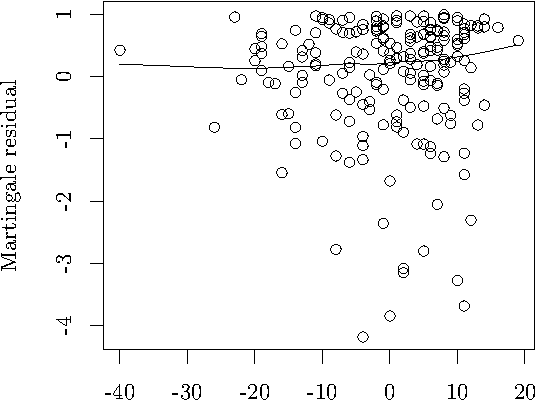
\includegraphics[width=\maxwidth]{figure/05-eda-func-form-age-1} 

}


\begin{kframe}\begin{alltt}
\hlkwd{scatter.smooth}\hlstd{(data}\hlopt{$}\hlstd{AgeCent,} \hlkwd{resid}\hlstd{(fit.cph.NoAge,} \hlkwc{type} \hlstd{=} \hlstr{"martingale"}\hlstd{),} \hlkwc{xlab} \hlstd{=} \hlstr{""}\hlstd{,} \hlkwc{ylab} \hlstd{=} \hlstr{"Martingale residual"}\hlstd{,} \hlkwc{ylim} \hlstd{=} \hlkwd{c}\hlstd{(}\hlopt{-}\hlnum{1}\hlstd{,} \hlnum{1}\hlstd{))}
\end{alltt}
\end{kframe}

{\centering 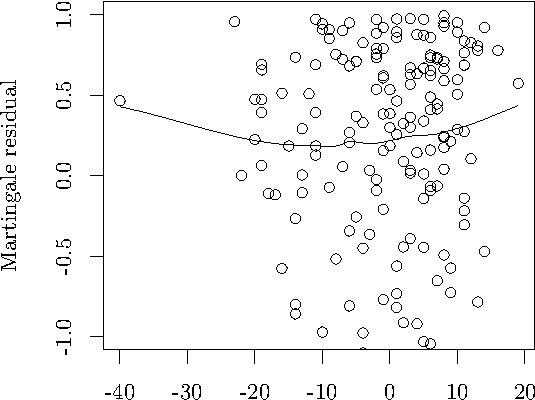
\includegraphics[width=\maxwidth]{figure/05-eda-func-form-age-2} 

}



\end{knitrout}
Close enough to linear.

\begin{knitrout}
\definecolor{shadecolor}{rgb}{0.969, 0.969, 0.969}\color{fgcolor}\begin{kframe}
\begin{alltt}
\hlstd{fit.cph.NoDate} \hlkwb{=} \hlkwd{coxph}\hlstd{(}\hlkwd{Surv}\hlstd{(Time, DSD)} \hlopt{~} \hlstd{SexM} \hlopt{+} \hlstd{AgeCent} \hlopt{+} \hlstd{LocBody} \hlopt{+} \hlstd{SizeCent} \hlopt{+} \hlstd{A2} \hlopt{+} \hlstd{A4,} \hlkwc{data} \hlstd{= data)}
\hlkwd{scatter.smooth}\hlstd{(data}\hlopt{$}\hlstd{DiagYearCent,} \hlkwd{resid}\hlstd{(fit.cph.NoDate,} \hlkwc{type} \hlstd{=} \hlstr{"martingale"}\hlstd{),} \hlkwc{xlab} \hlstd{=} \hlstr{""}\hlstd{,} \hlkwc{ylab} \hlstd{=} \hlstr{"Martingale residual"}\hlstd{)}
\end{alltt}
\end{kframe}

{\centering 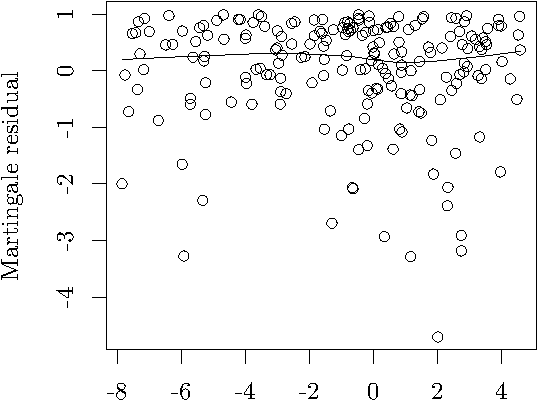
\includegraphics[width=\maxwidth]{figure/05-eda-func-form-date-1} 

}


\begin{kframe}\begin{alltt}
\hlkwd{scatter.smooth}\hlstd{(data}\hlopt{$}\hlstd{DiagYearCent,} \hlkwd{resid}\hlstd{(fit.cph.NoDate,} \hlkwc{type} \hlstd{=} \hlstr{"martingale"}\hlstd{),} \hlkwc{xlab} \hlstd{=} \hlstr{""}\hlstd{,} \hlkwc{ylab} \hlstd{=} \hlstr{"Martingale residual"}\hlstd{,} \hlkwc{ylim} \hlstd{=} \hlkwd{c}\hlstd{(}\hlopt{-}\hlnum{1}\hlstd{,} \hlnum{1}\hlstd{))}
\end{alltt}
\end{kframe}

{\centering 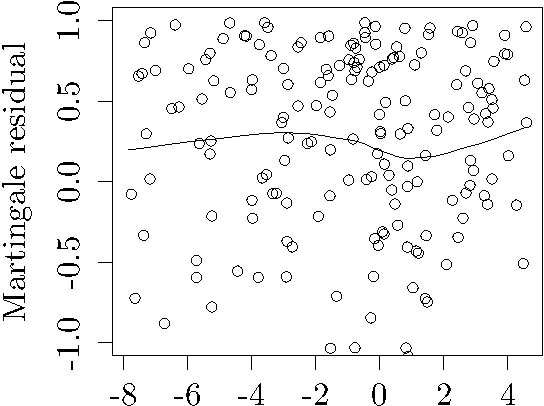
\includegraphics[width=\maxwidth]{figure/05-eda-func-form-date-2} 

}



\end{knitrout}
Doesn't appear to have much of an effect.

\begin{knitrout}
\definecolor{shadecolor}{rgb}{0.969, 0.969, 0.969}\color{fgcolor}\begin{kframe}
\begin{alltt}
\hlstd{fit.cph.NoSize} \hlkwb{=} \hlkwd{coxph}\hlstd{(}\hlkwd{Surv}\hlstd{(Time, DSD)} \hlopt{~} \hlstd{DiagYearCent} \hlopt{+} \hlstd{SexM} \hlopt{+} \hlstd{AgeCent} \hlopt{+} \hlstd{LocBody} \hlopt{+} \hlstd{A2} \hlopt{+} \hlstd{A4,} \hlkwc{data} \hlstd{= data)}
\hlkwd{scatter.smooth}\hlstd{(data}\hlopt{$}\hlstd{SizeCent,} \hlkwd{resid}\hlstd{(fit.cph.NoSize,} \hlkwc{type} \hlstd{=} \hlstr{"martingale"}\hlstd{),} \hlkwc{xlab} \hlstd{=} \hlstr{""}\hlstd{,} \hlkwc{ylab} \hlstd{=} \hlstr{"Martingale residual"}\hlstd{)}
\end{alltt}
\end{kframe}

{\centering 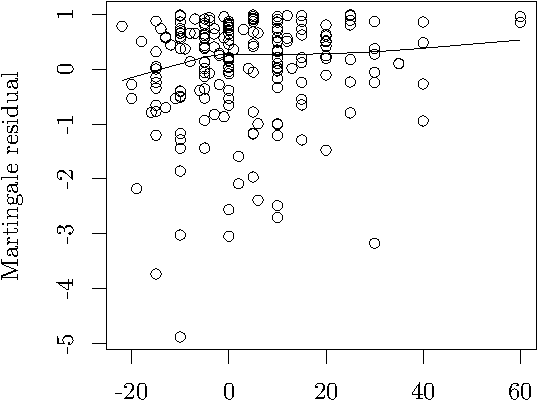
\includegraphics[width=\maxwidth]{figure/05-eda-func-form-size-1} 

}


\begin{kframe}\begin{alltt}
\hlkwd{scatter.smooth}\hlstd{(data}\hlopt{$}\hlstd{SizeCent,} \hlkwd{resid}\hlstd{(fit.cph.NoSize,} \hlkwc{type} \hlstd{=} \hlstr{"martingale"}\hlstd{),} \hlkwc{xlab} \hlstd{=} \hlstr{""}\hlstd{,} \hlkwc{ylab} \hlstd{=} \hlstr{"Martingale residual"}\hlstd{,} \hlkwc{ylim} \hlstd{=} \hlkwd{c}\hlstd{(}\hlopt{-}\hlnum{1}\hlstd{,} \hlnum{1}\hlstd{))}
\end{alltt}
\end{kframe}

{\centering 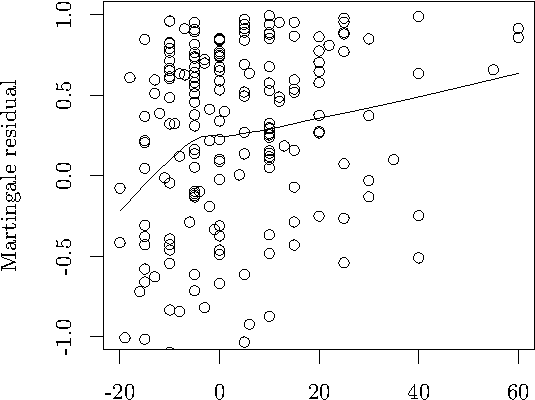
\includegraphics[width=\maxwidth]{figure/05-eda-func-form-size-2} 

}



\end{knitrout}
The size relationship appears to have a knee, close to size == 0, around which the relationship is approximately linear.

Model size as: $SizeCent + SizeCent I(SizeCent > 0) \equiv SizeCent + SizeCent_+$

\begin{knitrout}
\definecolor{shadecolor}{rgb}{0.969, 0.969, 0.969}\color{fgcolor}\begin{kframe}
\begin{alltt}
\hlstd{data}\hlopt{$}\hlstd{SizePlus} \hlkwb{=} \hlkwd{pmax}\hlstd{(data}\hlopt{$}\hlstd{SizeCent,} \hlnum{0}\hlstd{)}
\hlstd{data.val}\hlopt{$}\hlstd{SizePlus} \hlkwb{=} \hlkwd{pmax}\hlstd{(data.val}\hlopt{$}\hlstd{SizeCent,} \hlnum{0}\hlstd{)}
\hlstd{data.all}\hlopt{$}\hlstd{SizePlus} \hlkwb{=} \hlkwd{pmax}\hlstd{(data.all}\hlopt{$}\hlstd{SizeCent,} \hlnum{0}\hlstd{)}
\end{alltt}
\end{kframe}
\end{knitrout}


\subsection{PH assumption: full model}
\begin{knitrout}
\definecolor{shadecolor}{rgb}{0.969, 0.969, 0.969}\color{fgcolor}\begin{kframe}
\begin{alltt}
\hlstd{data.temp} \hlkwb{=} \hlstd{data}
\hlstd{data.temp}\hlopt{$}\hlstd{Time} \hlkwb{=} \hlstd{data.time}\hlopt{$}\hlstd{Time}\hlopt{/}\hlnum{365.25}\hlopt{*}\hlnum{12}
\end{alltt}


{\ttfamily\noindent\bfseries\color{errorcolor}{\#\# Error in eval(expr, envir, enclos): object 'data.time' not found}}\begin{alltt}
\hlstd{fit.cph} \hlkwb{=} \hlkwd{coxph}\hlstd{(}\hlkwd{Surv}\hlstd{(Time, DSD)} \hlopt{~} \hlstd{SexM} \hlopt{+} \hlstd{AgeCent} \hlopt{+} \hlstd{LocBody} \hlopt{+} \hlstd{SizeCent} \hlopt{+} \hlstd{SizePlus} \hlopt{+} \hlstd{A2} \hlopt{+} \hlstd{A4,} \hlkwc{data} \hlstd{= data.temp)}
\hlkwd{cox.zph}\hlstd{(fit.cph)}
\end{alltt}
\begin{verbatim}
##                  rho    chisq      p
## SexMTRUE     0.17964  6.56115 0.0104
## AgeCent     -0.10574  2.40668 0.1208
## LocBodyTRUE -0.04856  0.37895 0.5382
## SizeCent     0.00231  0.00106 0.9740
## SizePlus    -0.01130  0.02666 0.8703
## A2TRUE      -0.03995  0.29907 0.5845
## A4TRUE      -0.08343  1.33308 0.2483
## GLOBAL            NA 13.17267 0.0680
\end{verbatim}
\begin{alltt}
\hlstd{myplot.cox.zph} \hlkwb{=} \hlkwa{function}\hlstd{(}\hlkwc{x}\hlstd{,} \hlkwc{resid} \hlstd{=} \hlnum{TRUE}\hlstd{,} \hlkwc{se} \hlstd{=} \hlnum{TRUE}\hlstd{,} \hlkwc{df} \hlstd{=} \hlnum{4}\hlstd{,} \hlkwc{nsmo} \hlstd{=} \hlnum{40}\hlstd{,} \hlkwc{var}\hlstd{,} \hlkwc{...}\hlstd{)}
\hlstd{\{}
    \hlstd{xx} \hlkwb{<-} \hlstd{x}\hlopt{$}\hlstd{x}
    \hlstd{yy} \hlkwb{<-} \hlstd{x}\hlopt{$}\hlstd{y}
    \hlstd{d} \hlkwb{<-} \hlkwd{nrow}\hlstd{(yy)}
    \hlstd{df} \hlkwb{<-} \hlkwd{max}\hlstd{(df)}
    \hlstd{nvar} \hlkwb{<-} \hlkwd{ncol}\hlstd{(yy)}
    \hlstd{pred.x} \hlkwb{<-} \hlkwd{seq}\hlstd{(}\hlkwc{from} \hlstd{=} \hlkwd{min}\hlstd{(xx),} \hlkwc{to} \hlstd{=} \hlkwd{max}\hlstd{(xx),} \hlkwc{length} \hlstd{= nsmo)}
    \hlstd{temp} \hlkwb{<-} \hlkwd{c}\hlstd{(pred.x, xx)}
    \hlstd{lmat} \hlkwb{<-} \hlkwd{ns}\hlstd{(temp,} \hlkwc{df} \hlstd{= df,} \hlkwc{intercept} \hlstd{=} \hlnum{TRUE}\hlstd{)}
    \hlstd{pmat} \hlkwb{<-} \hlstd{lmat[}\hlnum{1}\hlopt{:}\hlstd{nsmo, ]}
    \hlstd{xmat} \hlkwb{<-} \hlstd{lmat[}\hlopt{-}\hlstd{(}\hlnum{1}\hlopt{:}\hlstd{nsmo), ]}
    \hlstd{qmat} \hlkwb{<-} \hlkwd{qr}\hlstd{(xmat)}
    \hlkwa{if} \hlstd{(qmat}\hlopt{$}\hlstd{rank} \hlopt{<} \hlstd{df)}
        \hlkwd{stop}\hlstd{(}\hlstr{"Spline fit is singular, try a smaller degrees of freedom"}\hlstd{)}
    \hlkwa{if} \hlstd{(se) \{}
        \hlstd{bk} \hlkwb{<-} \hlkwd{backsolve}\hlstd{(qmat}\hlopt{$}\hlstd{qr[}\hlnum{1}\hlopt{:}\hlstd{df,} \hlnum{1}\hlopt{:}\hlstd{df],} \hlkwd{diag}\hlstd{(df))}
        \hlstd{xtx} \hlkwb{<-} \hlstd{bk} \hlopt \hlkwd{t}\hlstd{(bk)}
        \hlstd{seval} \hlkwb{<-} \hlstd{d} \hlopt{*} \hlstd{((pmat} \hlopt \hlstd{xtx)} \hlopt{*} \hlstd{pmat)} \hlopt \hlkwd{rep}\hlstd{(}\hlnum{1}\hlstd{, df)}
    \hlstd{\}}
    \hlkwa{if} \hlstd{(}\hlkwd{missing}\hlstd{(var))}
        \hlstd{var} \hlkwb{<-} \hlnum{1}\hlopt{:}\hlstd{nvar}
    \hlkwa{else} \hlstd{\{}
        \hlkwa{if} \hlstd{(}\hlkwd{is.character}\hlstd{(var))}
            \hlstd{var} \hlkwb{<-} \hlkwd{match}\hlstd{(var,} \hlkwd{dimnames}\hlstd{(yy)[[}\hlnum{2}\hlstd{]])}
        \hlkwa{if} \hlstd{(}\hlkwd{any}\hlstd{(}\hlkwd{is.na}\hlstd{(var))} \hlopt{||} \hlkwd{max}\hlstd{(var)} \hlopt{>} \hlstd{nvar} \hlopt{||} \hlkwd{min}\hlstd{(var)} \hlopt{<}
            \hlnum{1}\hlstd{)}
            \hlkwd{stop}\hlstd{(}\hlstr{"Invalid variable requested"}\hlstd{)}
    \hlstd{\}}
    \hlkwa{if} \hlstd{(x}\hlopt{$}\hlstd{transform} \hlopt{==} \hlstr{"log"}\hlstd{) \{}
        \hlstd{xx} \hlkwb{<-} \hlkwd{exp}\hlstd{(xx)}
        \hlstd{pred.x} \hlkwb{<-} \hlkwd{exp}\hlstd{(pred.x)}
    \hlstd{\}}
    \hlkwa{else if} \hlstd{(x}\hlopt{$}\hlstd{transform} \hlopt{!=} \hlstr{"identity"}\hlstd{) \{}
        \hlstd{xtime} \hlkwb{<-} \hlkwd{as.numeric}\hlstd{(}\hlkwd{dimnames}\hlstd{(yy)[[}\hlnum{1}\hlstd{]])}
        \hlstd{indx} \hlkwb{<-} \hlopt{!}\hlkwd{duplicated}\hlstd{(xx)}
        \hlstd{apr1} \hlkwb{<-} \hlkwd{approx}\hlstd{(xx[indx], xtime[indx],} \hlkwd{seq}\hlstd{(}\hlkwd{min}\hlstd{(xx),} \hlkwd{max}\hlstd{(xx),}
            \hlkwc{length} \hlstd{=} \hlnum{17}\hlstd{)[}\hlnum{2} \hlopt{*} \hlstd{(}\hlnum{1}\hlopt{:}\hlnum{8}\hlstd{)])}
        \hlstd{temp} \hlkwb{<-} \hlkwd{signif}\hlstd{(apr1}\hlopt{$}\hlstd{y,} \hlnum{2}\hlstd{)}
        \hlstd{apr2} \hlkwb{<-} \hlkwd{approx}\hlstd{(xtime[indx], xx[indx], temp)}
        \hlstd{xaxisval} \hlkwb{<-} \hlstd{apr2}\hlopt{$}\hlstd{y}
        \hlstd{xaxislab} \hlkwb{<-} \hlkwd{rep}\hlstd{(}\hlstr{""}\hlstd{,} \hlnum{8}\hlstd{)}
        \hlkwa{for} \hlstd{(i} \hlkwa{in} \hlnum{1}\hlopt{:}\hlnum{8}\hlstd{) xaxislab[i]} \hlkwb{<-} \hlkwd{format}\hlstd{(temp[i])}
    \hlstd{\}}
    \hlkwa{for} \hlstd{(i} \hlkwa{in} \hlstd{var) \{}
        \hlstd{y} \hlkwb{<-} \hlstd{yy[, i]}
        \hlstd{yhat} \hlkwb{<-} \hlstd{pmat} \hlopt \hlkwd{qr.coef}\hlstd{(qmat, y)}
        \hlkwa{if} \hlstd{(resid)}
            \hlstd{yr} \hlkwb{<-} \hlkwd{range}\hlstd{(yhat, y)}
        \hlkwa{else} \hlstd{yr} \hlkwb{<-} \hlkwd{range}\hlstd{(yhat)}
        \hlkwa{if} \hlstd{(se) \{}
            \hlstd{temp} \hlkwb{<-} \hlnum{2} \hlopt{*} \hlkwd{sqrt}\hlstd{(x}\hlopt{$}\hlstd{var[i, i]} \hlopt{*} \hlstd{seval)}
            \hlstd{yup} \hlkwb{<-} \hlstd{yhat} \hlopt{+} \hlstd{temp}
            \hlstd{ylow} \hlkwb{<-} \hlstd{yhat} \hlopt{-} \hlstd{temp}
            \hlstd{yr} \hlkwb{<-} \hlkwd{range}\hlstd{(yr, yup, ylow)}
        \hlstd{\}}
        \hlkwa{if} \hlstd{(x}\hlopt{$}\hlstd{transform} \hlopt{==} \hlstr{"identity"}\hlstd{)}
            \hlkwd{plot}\hlstd{(}\hlkwd{range}\hlstd{(xx), yr,} \hlkwc{type} \hlstd{=} \hlstr{"n"}\hlstd{, ...)}
        \hlkwa{else if} \hlstd{(x}\hlopt{$}\hlstd{transform} \hlopt{==} \hlstr{"log"}\hlstd{)}
            \hlkwd{plot}\hlstd{(}\hlkwd{range}\hlstd{(xx), yr,} \hlkwc{type} \hlstd{=} \hlstr{"n"}\hlstd{,} \hlkwc{log} \hlstd{=} \hlstr{"x"}\hlstd{, ...)}
        \hlkwa{else} \hlstd{\{}
            \hlkwd{plot}\hlstd{(}\hlkwd{range}\hlstd{(xx), yr,} \hlkwc{type} \hlstd{=} \hlstr{"n"}\hlstd{,} \hlkwc{axes} \hlstd{=} \hlnum{FALSE}\hlstd{, ...)}
            \hlkwd{axis}\hlstd{(}\hlnum{1}\hlstd{, xaxisval, xaxislab)}
            \hlkwd{axis}\hlstd{(}\hlnum{2}\hlstd{)}
            \hlkwd{box}\hlstd{()}
        \hlstd{\}}
        \hlkwa{if} \hlstd{(resid)}
            \hlkwd{points}\hlstd{(xx, y)}
        \hlkwd{lines}\hlstd{(pred.x, yhat)}
        \hlkwa{if} \hlstd{(se) \{}
            \hlkwd{lines}\hlstd{(pred.x, yup,} \hlkwc{lty} \hlstd{=} \hlnum{2}\hlstd{)}
            \hlkwd{lines}\hlstd{(pred.x, ylow,} \hlkwc{lty} \hlstd{=} \hlnum{2}\hlstd{)}
        \hlstd{\}}
    \hlstd{\}}
\hlstd{\}}

\hlkwd{myplot.cox.zph}\hlstd{(}\hlkwd{cox.zph}\hlstd{(fit.cph)[}\hlnum{1}\hlstd{],} \hlkwc{xlab} \hlstd{=} \hlstr{"Time (months)"}\hlstd{,} \hlkwc{ylab} \hlstd{=} \hlstr{"Beta(t) for Sex = Male"}\hlstd{)}
\end{alltt}
\end{kframe}

{\centering 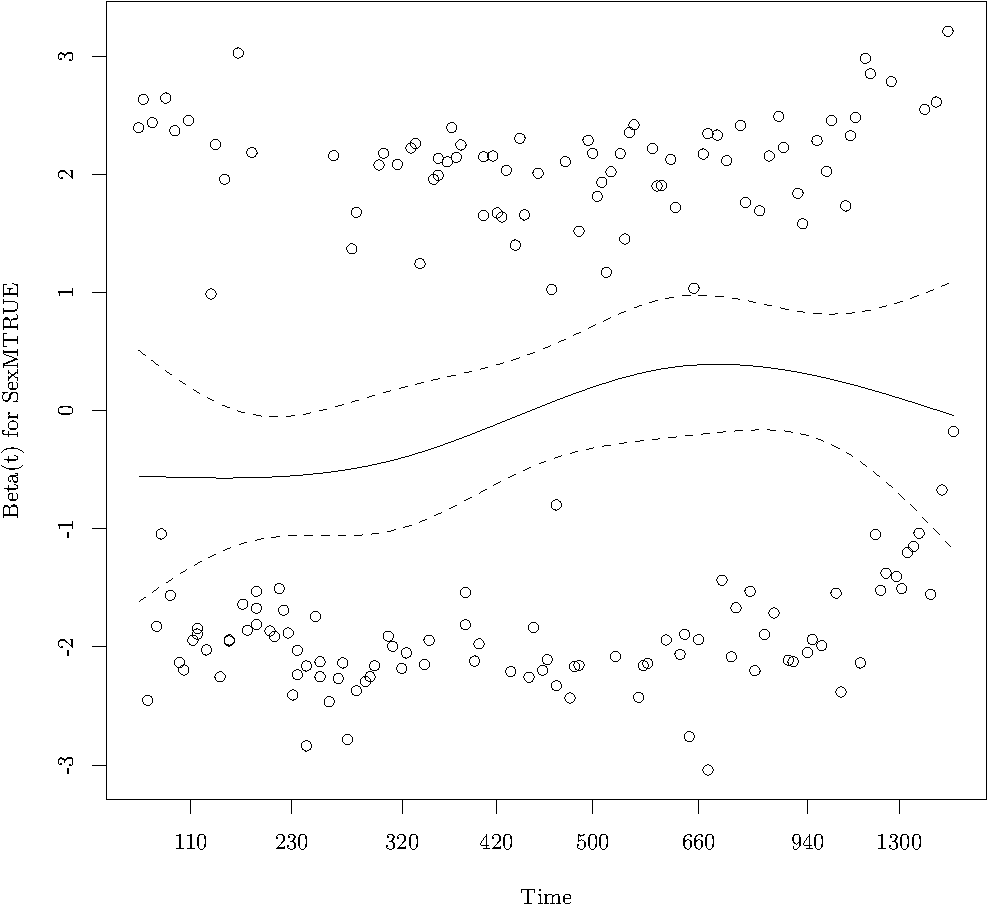
\includegraphics[width=\maxwidth]{figure/05-eda-ph-check-full-1} 

}


\begin{kframe}\begin{alltt}
\hlstd{fit.cph} \hlkwb{=} \hlkwd{coxph}\hlstd{(}\hlkwd{Surv}\hlstd{(Time, DSD)} \hlopt{~} \hlkwd{strata}\hlstd{(SexM)} \hlopt{+} \hlstd{AgeCent} \hlopt{+} \hlstd{LocBody} \hlopt{+} \hlstd{SizeCent} \hlopt{+} \hlstd{SizePlus} \hlopt{+} \hlstd{A2} \hlopt{+} \hlstd{A4,} \hlkwc{data} \hlstd{= data)}
\hlkwd{cox.zph}\hlstd{(fit.cph)}
\end{alltt}
\begin{verbatim}
##                  rho   chisq      p
## AgeCent     -0.11339 2.78186 0.0953
## LocBodyTRUE -0.04618 0.34177 0.5588
## SizeCent     0.00662 0.00857 0.9262
## SizePlus    -0.01329 0.03588 0.8498
## A2TRUE      -0.04361 0.35772 0.5498
## A4TRUE      -0.07985 1.25354 0.2629
## GLOBAL            NA 6.03352 0.4194
\end{verbatim}
\end{kframe}
\end{knitrout}
Using a threshold of 0.1 for the CPH tests, sex is stuffing things up.  Stratification by sex makes good sense, given known variation in survival between the sexes.  It would have been possible to model this with a Sex:Age term in an AFT model, but given this is CPH, a baseline change is needed.


\subsection{Date of diagnosis test}
\begin{knitrout}
\definecolor{shadecolor}{rgb}{0.969, 0.969, 0.969}\color{fgcolor}\begin{kframe}
\begin{alltt}
\hlstd{temp1} \hlkwb{=} \hlkwd{coxph}\hlstd{(}\hlkwd{Surv}\hlstd{(Time, DSD)} \hlopt{~} \hlkwd{strata}\hlstd{(SexM)} \hlopt{+} \hlstd{AgeCent} \hlopt{+} \hlstd{LocBody} \hlopt{+} \hlstd{SizeCent} \hlopt{+} \hlstd{SizePlus} \hlopt{+} \hlstd{A2} \hlopt{+} \hlstd{A4,} \hlkwc{data} \hlstd{= data)}
\hlstd{temp2} \hlkwb{=} \hlkwd{coxph}\hlstd{(}\hlkwd{Surv}\hlstd{(Time, DSD)} \hlopt{~} \hlkwd{strata}\hlstd{(SexM)} \hlopt{+} \hlstd{AgeCent} \hlopt{+} \hlstd{LocBody} \hlopt{+} \hlstd{SizeCent} \hlopt{+} \hlstd{SizePlus} \hlopt{+} \hlstd{A2} \hlopt{+} \hlstd{A4} \hlopt{+} \hlstd{DiagYearCent,} \hlkwc{data} \hlstd{= data)}
\hlkwd{anova}\hlstd{(temp1, temp2)}
\end{alltt}
\begin{verbatim}
## Analysis of Deviance Table
##  Cox model: response is  Surv(Time, DSD)
##  Model 1: ~ strata(SexM) + AgeCent + LocBody + SizeCent + SizePlus + A2 + A4
##  Model 2: ~ strata(SexM) + AgeCent + LocBody + SizeCent + SizePlus + A2 + A4 + DiagYearCent
##   loglik Chisq Df P(>|Chi|)
## 1   -682                   
## 2   -682  0.86  1      0.35
\end{verbatim}
\begin{alltt}
\hlkwd{library}\hlstd{(energy)}

\hlkwd{scatter.smooth}\hlstd{(data}\hlopt{$}\hlstd{DiagYearCent, data}\hlopt{$}\hlstd{SexM,} \hlkwc{xlab} \hlstd{=} \hlstr{"DiagYearCent"}\hlstd{,} \hlkwc{ylab} \hlstd{=} \hlstr{"SexM"}\hlstd{)}
\end{alltt}
\end{kframe}

{\centering 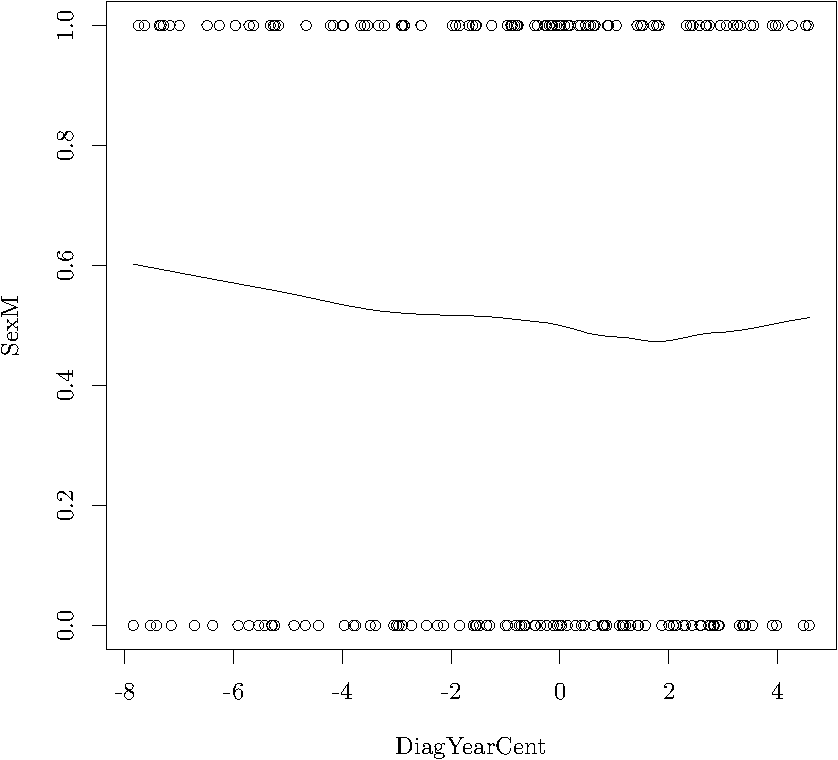
\includegraphics[width=\maxwidth]{figure/05-eda-dod-check-1} 

}


\begin{kframe}\begin{alltt}
\hlkwd{boxplot}\hlstd{(DiagYearCent} \hlopt{~} \hlstd{SexM, data)}
\end{alltt}
\end{kframe}

{\centering 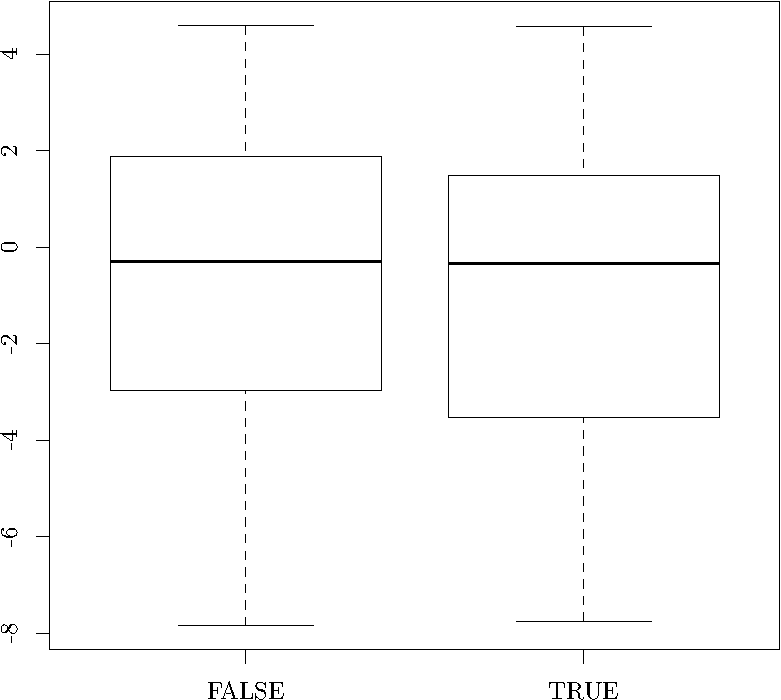
\includegraphics[width=\maxwidth]{figure/05-eda-dod-check-2} 

}


\begin{kframe}\begin{alltt}
\hlkwd{kruskal.test}\hlstd{(data}\hlopt{$}\hlstd{DiagYearCent, data}\hlopt{$}\hlstd{SexM)}
\end{alltt}
\begin{verbatim}
## 
## 	Kruskal-Wallis rank sum test
## 
## data:  data$DiagYearCent and data$SexM
## Kruskal-Wallis chi-squared = 0.4306, df = 1, p-value = 0.5117
\end{verbatim}
\begin{alltt}
\hlkwd{dcov.test}\hlstd{(data}\hlopt{$}\hlstd{DiagYearCent, data}\hlopt{$}\hlstd{SexM,} \hlkwc{R} \hlstd{=} \hlnum{499}\hlstd{)}
\end{alltt}
\begin{verbatim}
## 
## 	dCov test of independence
## 
## data:  index 1, replicates 499
## nV^2 = 0.7729, p-value = 0.784
## sample estimates:
##    dCov 
## 0.06217
\end{verbatim}
\begin{alltt}
\hlkwd{scatter.smooth}\hlstd{(data}\hlopt{$}\hlstd{DiagYearCent, data}\hlopt{$}\hlstd{AgeCent,} \hlkwc{xlab} \hlstd{=} \hlstr{"DiagYearCent"}\hlstd{,} \hlkwc{ylab} \hlstd{=} \hlstr{"AgeCent"}\hlstd{)}
\end{alltt}
\end{kframe}

{\centering 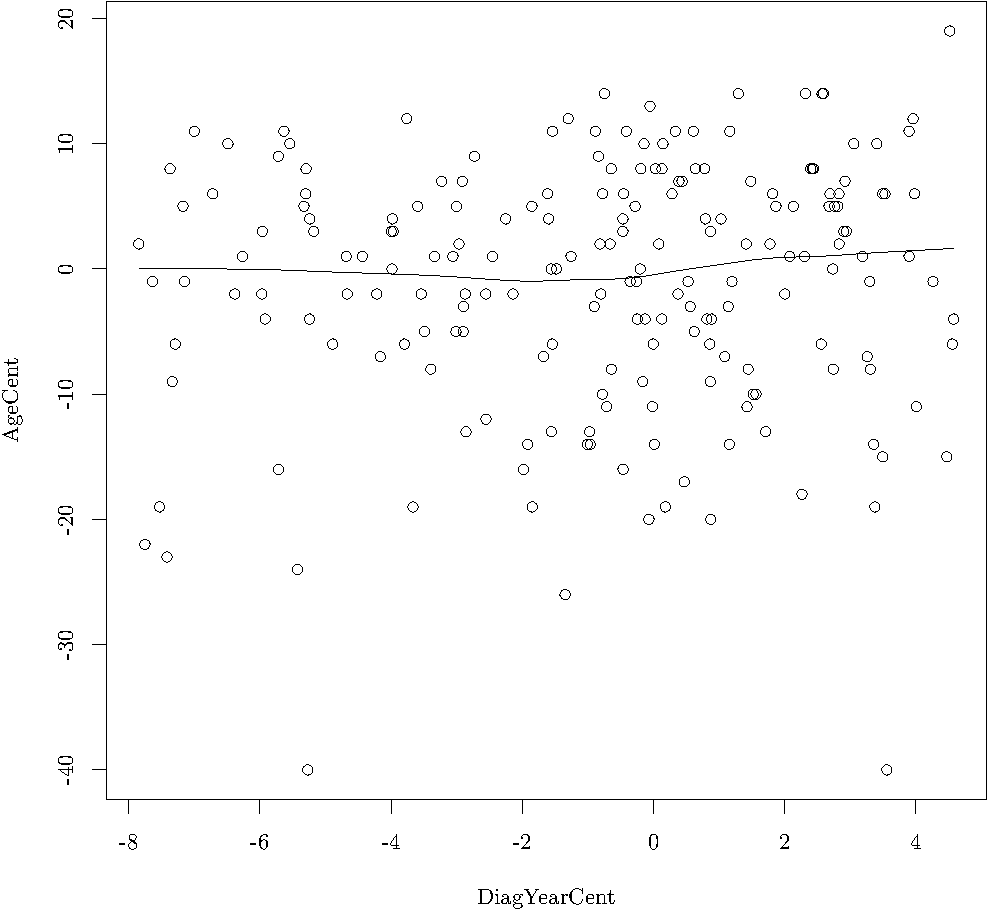
\includegraphics[width=\maxwidth]{figure/05-eda-dod-check-3} 

}


\begin{kframe}\begin{alltt}
\hlkwd{cor.test}\hlstd{(data}\hlopt{$}\hlstd{DiagYearCent, data}\hlopt{$}\hlstd{AgeCent,} \hlkwc{method} \hlstd{=} \hlstr{"kendall"}\hlstd{)}
\end{alltt}
\begin{verbatim}
## 
## 	Kendall's rank correlation tau
## 
## data:  data$DiagYearCent and data$AgeCent
## z = 1.026, p-value = 0.3049
## alternative hypothesis: true tau is not equal to 0
## sample estimates:
##     tau 
## 0.04952
\end{verbatim}
\begin{alltt}
\hlkwd{dcov.test}\hlstd{(data}\hlopt{$}\hlstd{DiagYearCent, data}\hlopt{$}\hlstd{AgeCent,} \hlkwc{R} \hlstd{=} \hlnum{499}\hlstd{)}
\end{alltt}
\begin{verbatim}
## 
## 	dCov test of independence
## 
## data:  index 1, replicates 499
## nV^2 = 36.72, p-value = 0.448
## sample estimates:
##   dCov 
## 0.4285
\end{verbatim}
\begin{alltt}
\hlkwd{scatter.smooth}\hlstd{(data}\hlopt{$}\hlstd{DiagYearCent, data}\hlopt{$}\hlstd{LocBody,} \hlkwc{xlab} \hlstd{=} \hlstr{"DiagYearCent"}\hlstd{,} \hlkwc{ylab} \hlstd{=} \hlstr{"LocBody"}\hlstd{)}
\end{alltt}
\end{kframe}

{\centering 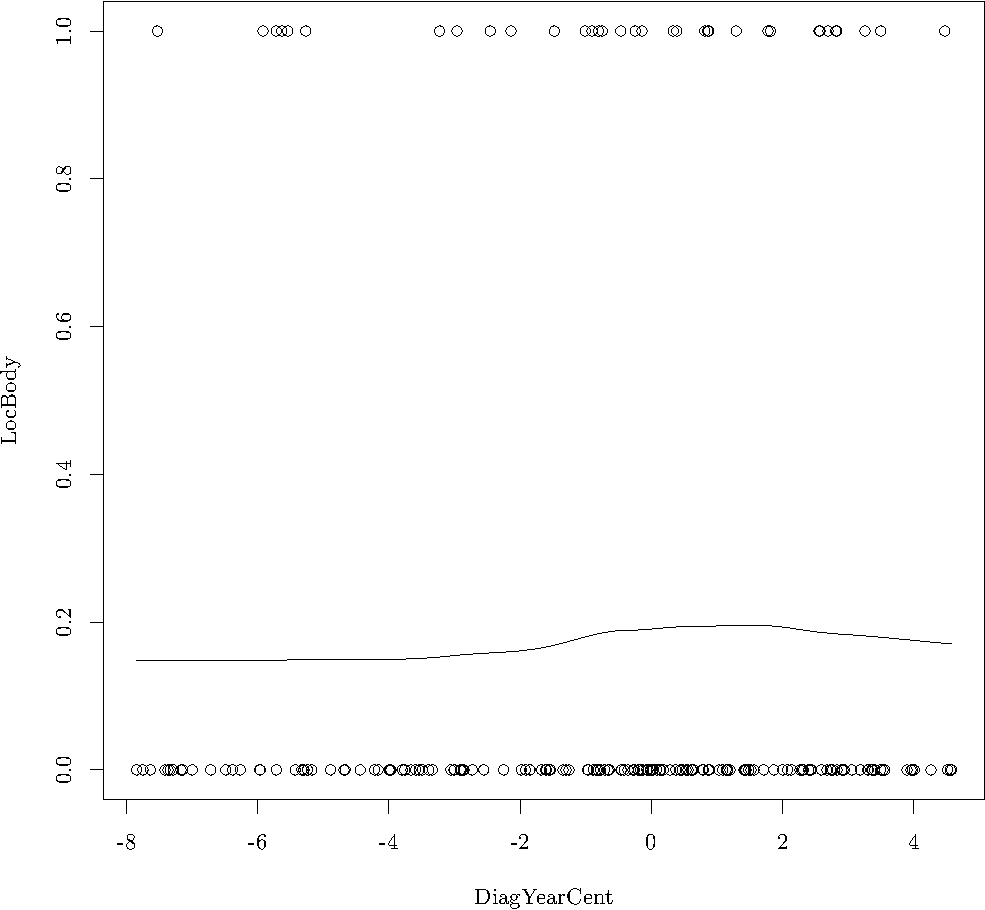
\includegraphics[width=\maxwidth]{figure/05-eda-dod-check-4} 

}


\begin{kframe}\begin{alltt}
\hlkwd{boxplot}\hlstd{(DiagYearCent} \hlopt{~} \hlstd{LocBody, data)}
\end{alltt}
\end{kframe}

{\centering 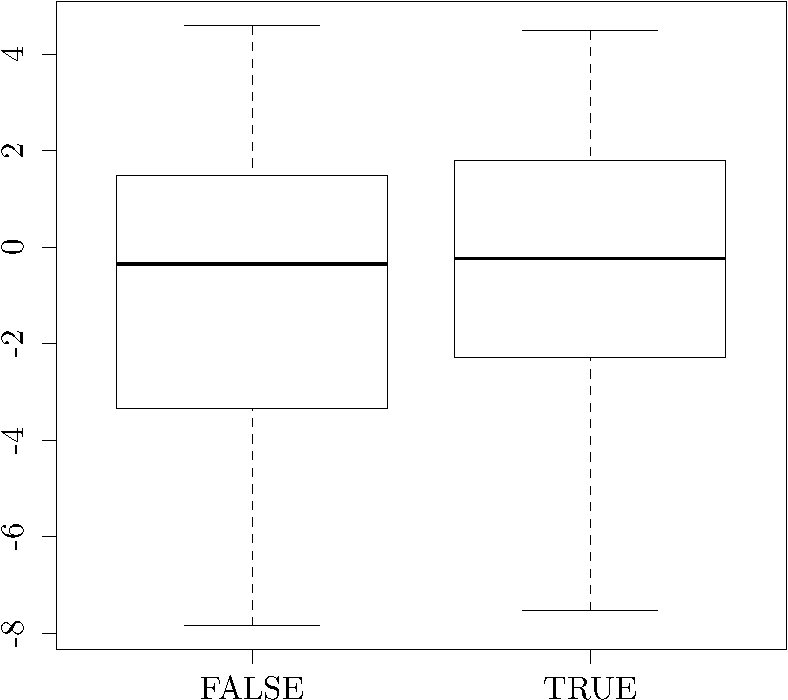
\includegraphics[width=\maxwidth]{figure/05-eda-dod-check-5} 

}


\begin{kframe}\begin{alltt}
\hlkwd{kruskal.test}\hlstd{(data}\hlopt{$}\hlstd{DiagYearCent, data}\hlopt{$}\hlstd{LocBody)}
\end{alltt}
\begin{verbatim}
## 
## 	Kruskal-Wallis rank sum test
## 
## data:  data$DiagYearCent and data$LocBody
## Kruskal-Wallis chi-squared = 0.2357, df = 1, p-value = 0.6273
\end{verbatim}
\begin{alltt}
\hlkwd{dcov.test}\hlstd{(data}\hlopt{$}\hlstd{DiagYearCent, data}\hlopt{$}\hlstd{LocBody,} \hlkwc{R} \hlstd{=} \hlnum{499}\hlstd{)}
\end{alltt}
\begin{verbatim}
## 
## 	dCov test of independence
## 
## data:  index 1, replicates 499
## nV^2 = 0.4203, p-value = 0.812
## sample estimates:
##    dCov 
## 0.04584
\end{verbatim}
\begin{alltt}
\hlkwd{scatter.smooth}\hlstd{(data}\hlopt{$}\hlstd{DiagYearCent, data}\hlopt{$}\hlstd{SizeCent,} \hlkwc{xlab} \hlstd{=} \hlstr{"DiagYearCent"}\hlstd{,} \hlkwc{ylab} \hlstd{=} \hlstr{"SizeCent"}\hlstd{)}
\end{alltt}
\end{kframe}

{\centering 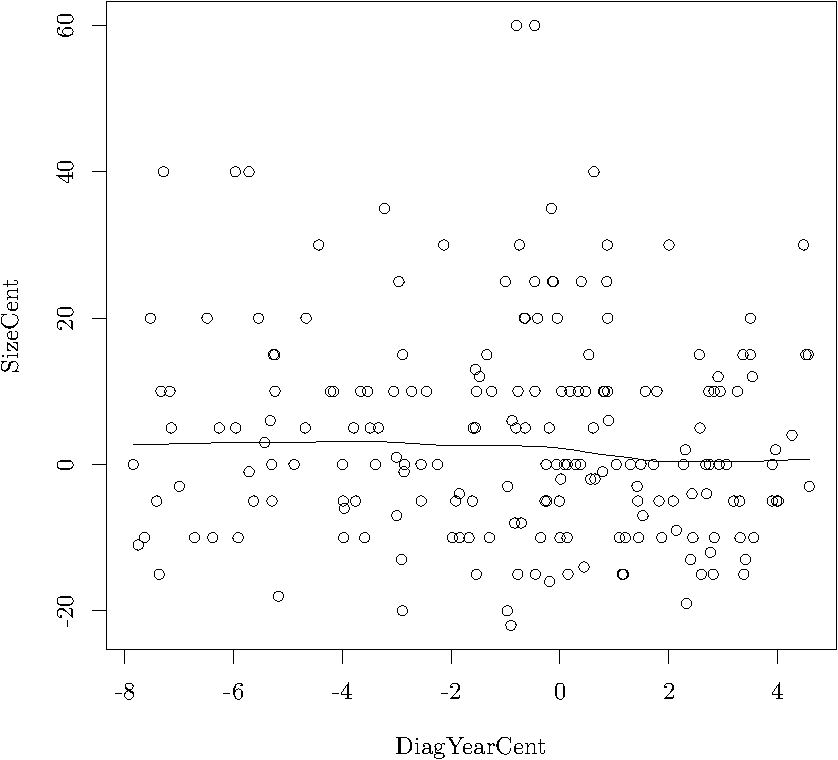
\includegraphics[width=\maxwidth]{figure/05-eda-dod-check-6} 

}


\begin{kframe}\begin{alltt}
\hlkwd{cor.test}\hlstd{(data}\hlopt{$}\hlstd{DiagYearCent, data}\hlopt{$}\hlstd{SizeCent,} \hlkwc{method} \hlstd{=} \hlstr{"kendall"}\hlstd{)}
\end{alltt}
\begin{verbatim}
## 
## 	Kendall's rank correlation tau
## 
## data:  data$DiagYearCent and data$SizeCent
## z = -1.095, p-value = 0.2737
## alternative hypothesis: true tau is not equal to 0
## sample estimates:
##      tau 
## -0.05367
\end{verbatim}
\begin{alltt}
\hlkwd{dcov.test}\hlstd{(data}\hlopt{$}\hlstd{DiagYearCent, data}\hlopt{$}\hlstd{SizeCent,} \hlkwc{R} \hlstd{=} \hlnum{499}\hlstd{)}
\end{alltt}
\begin{verbatim}
## 
## 	dCov test of independence
## 
## data:  index 1, replicates 499
## nV^2 = 59.67, p-value = 0.372
## sample estimates:
##   dCov 
## 0.5462
\end{verbatim}
\begin{alltt}
\hlkwd{scatter.smooth}\hlstd{(data}\hlopt{$}\hlstd{DiagYearCent, data}\hlopt{$}\hlstd{A2,} \hlkwc{xlab} \hlstd{=} \hlstr{"DiagYearCent"}\hlstd{,} \hlkwc{ylab} \hlstd{=} \hlstr{"A2"}\hlstd{)}
\end{alltt}
\end{kframe}

{\centering 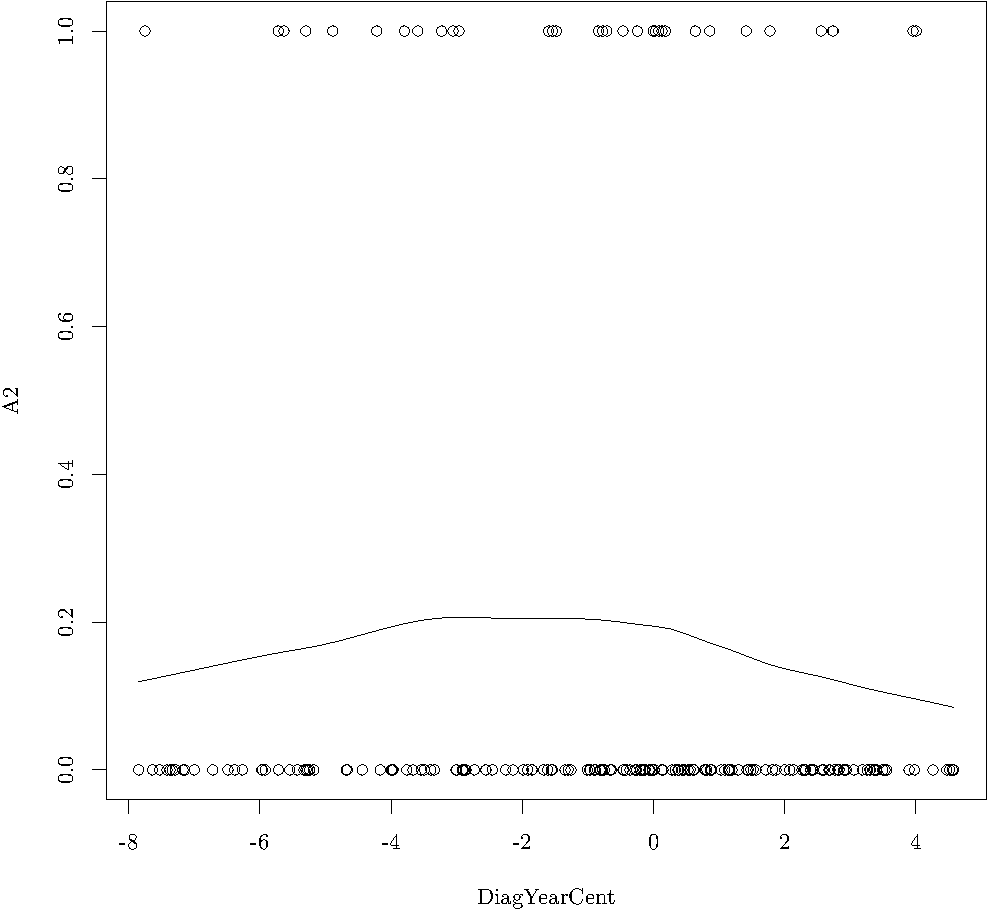
\includegraphics[width=\maxwidth]{figure/05-eda-dod-check-7} 

}


\begin{kframe}\begin{alltt}
\hlkwd{boxplot}\hlstd{(DiagYearCent} \hlopt{~} \hlstd{A2, data)}
\end{alltt}
\end{kframe}

{\centering 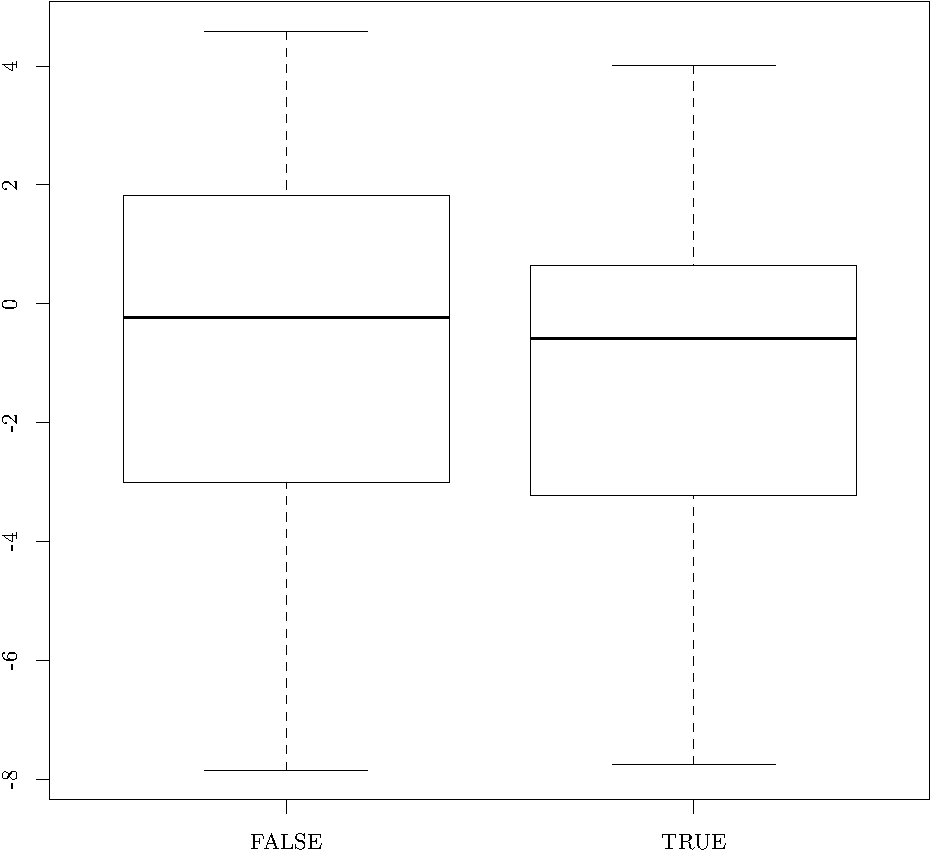
\includegraphics[width=\maxwidth]{figure/05-eda-dod-check-8} 

}


\begin{kframe}\begin{alltt}
\hlkwd{kruskal.test}\hlstd{(data}\hlopt{$}\hlstd{DiagYearCent, data}\hlopt{$}\hlstd{A2)}
\end{alltt}
\begin{verbatim}
## 
## 	Kruskal-Wallis rank sum test
## 
## data:  data$DiagYearCent and data$A2
## Kruskal-Wallis chi-squared = 0.5693, df = 1, p-value = 0.4505
\end{verbatim}
\begin{alltt}
\hlkwd{dcov.test}\hlstd{(data}\hlopt{$}\hlstd{DiagYearCent, data}\hlopt{$}\hlstd{A2,} \hlkwc{R} \hlstd{=} \hlnum{499}\hlstd{)}
\end{alltt}
\begin{verbatim}
## 
## 	dCov test of independence
## 
## data:  index 1, replicates 499
## nV^2 = 0.6903, p-value = 0.558
## sample estimates:
##    dCov 
## 0.05875
\end{verbatim}
\begin{alltt}
\hlkwd{scatter.smooth}\hlstd{(data}\hlopt{$}\hlstd{DiagYearCent, data}\hlopt{$}\hlstd{A4,} \hlkwc{xlab} \hlstd{=} \hlstr{"DiagYearCent"}\hlstd{,} \hlkwc{ylab} \hlstd{=} \hlstr{"A4"}\hlstd{)}
\end{alltt}
\end{kframe}

{\centering 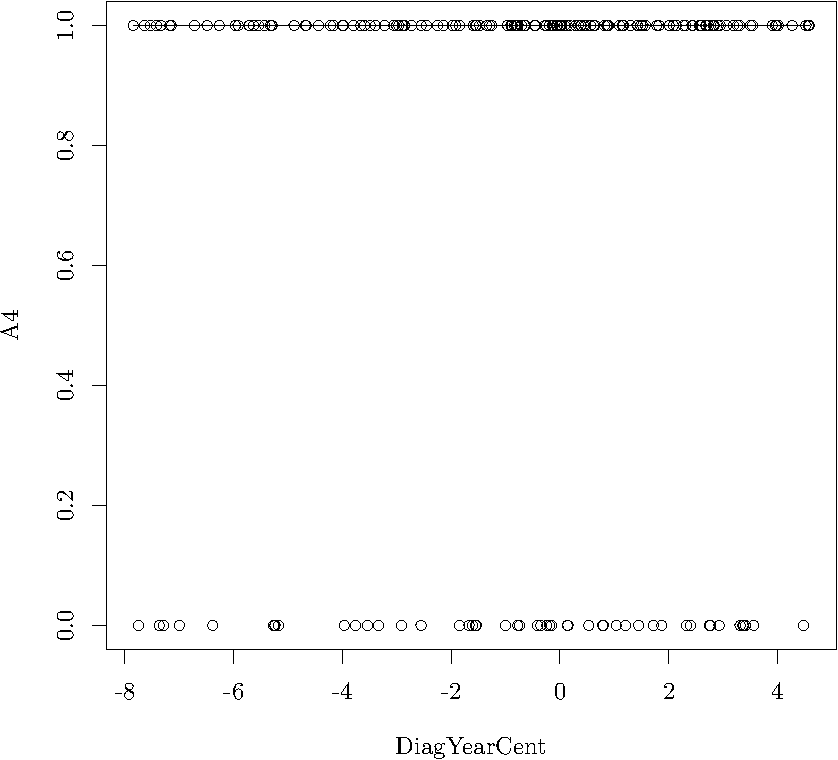
\includegraphics[width=\maxwidth]{figure/05-eda-dod-check-9} 

}


\begin{kframe}\begin{alltt}
\hlkwd{boxplot}\hlstd{(DiagYearCent} \hlopt{~} \hlstd{A4, data)}
\end{alltt}
\end{kframe}

{\centering 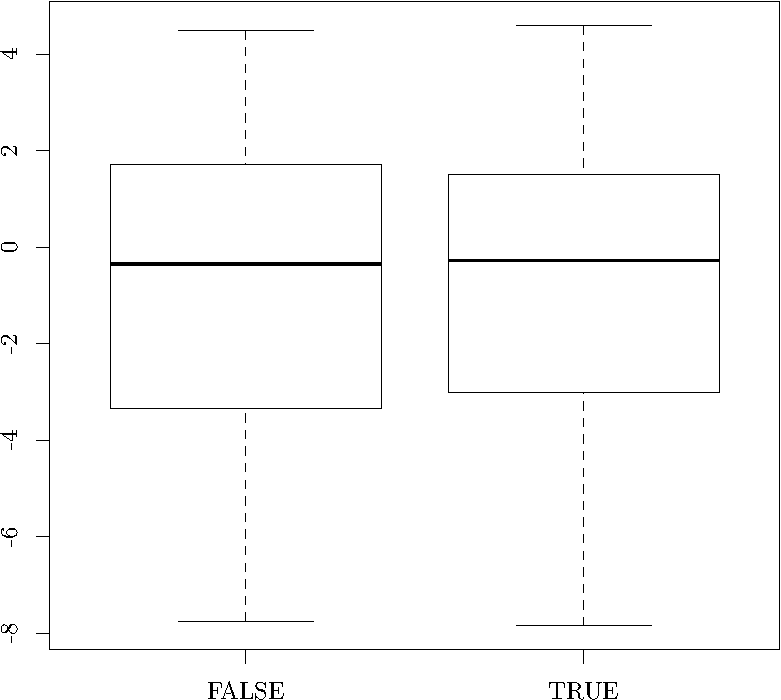
\includegraphics[width=\maxwidth]{figure/05-eda-dod-check-10} 

}


\begin{kframe}\begin{alltt}
\hlkwd{kruskal.test}\hlstd{(data}\hlopt{$}\hlstd{DiagYearCent, data}\hlopt{$}\hlstd{A4)}
\end{alltt}
\begin{verbatim}
## 
## 	Kruskal-Wallis rank sum test
## 
## data:  data$DiagYearCent and data$A4
## Kruskal-Wallis chi-squared = 0.0055, df = 1, p-value = 0.9411
\end{verbatim}
\begin{alltt}
\hlkwd{dcov.test}\hlstd{(data}\hlopt{$}\hlstd{DiagYearCent, data}\hlopt{$}\hlstd{A4,} \hlkwc{R} \hlstd{=} \hlnum{499}\hlstd{)}
\end{alltt}
\begin{verbatim}
## 
## 	dCov test of independence
## 
## data:  index 1, replicates 499
## nV^2 = 0.1731, p-value = 0.998
## sample estimates:
##    dCov 
## 0.02942
\end{verbatim}
\end{kframe}
\end{knitrout}
Not significant; good.


\subsection{Outliers}
\begin{knitrout}
\definecolor{shadecolor}{rgb}{0.969, 0.969, 0.969}\color{fgcolor}\begin{kframe}
\begin{alltt}
\hlkwd{plot}\hlstd{(}\hlkwd{resid}\hlstd{(fit.cph,} \hlstr{"deviance"}\hlstd{))}
\hlkwd{abline}\hlstd{(}\hlkwc{h} \hlstd{=} \hlkwd{c}\hlstd{(}\hlopt{-}\hlnum{2}\hlstd{,} \hlnum{2}\hlstd{))}
\end{alltt}
\end{kframe}

{\centering 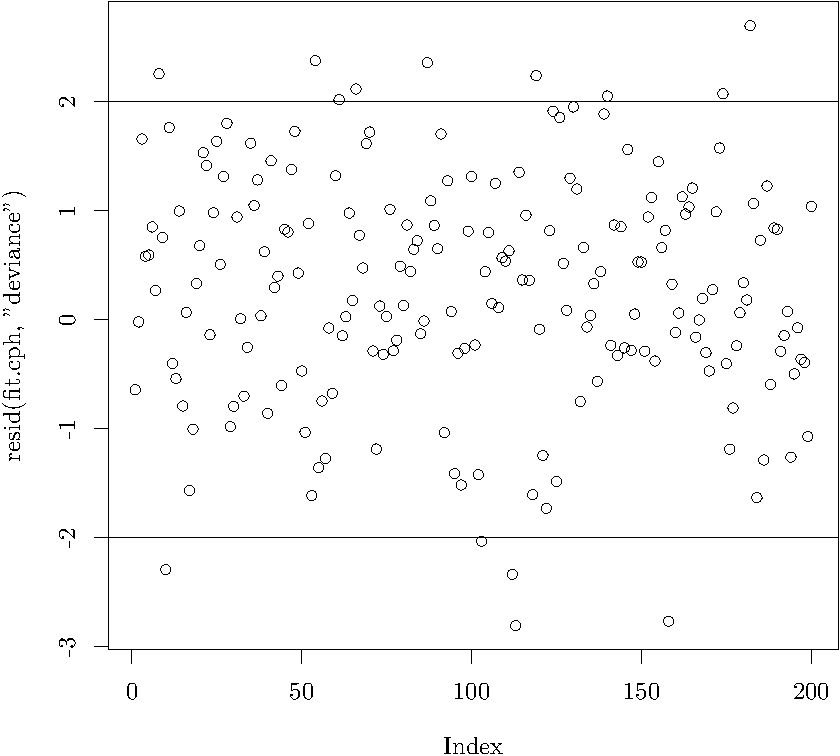
\includegraphics[width=\maxwidth]{figure/05-eda-outliers-1} 

}


\begin{kframe}\begin{alltt}
\hlstd{data}\hlopt{$}\hlstd{devresid} \hlkwb{=} \hlkwd{resid}\hlstd{(fit.cph,} \hlkwc{type} \hlstd{=} \hlstr{"deviance"}\hlstd{)}
\hlstd{temp} \hlkwb{=} \hlstd{data[}\hlkwd{abs}\hlstd{(data}\hlopt{$}\hlstd{devresid)} \hlopt{>=} \hlnum{2}\hlstd{,]}
\hlcom{#temp[order(temp$Time),]}

\hlstd{temp} \hlkwb{=} \hlkwd{resid}\hlstd{(fit.cph,} \hlkwc{type} \hlstd{=} \hlstr{"dfbetas"}\hlstd{)}
\hlkwd{colnames}\hlstd{(temp)} \hlkwb{=} \hlkwd{names}\hlstd{(fit.cph}\hlopt{$}\hlstd{coefficients)}
\hlstd{temp} \hlkwb{=} \hlkwd{melt}\hlstd{(temp)}
\hlkwd{colnames}\hlstd{(temp)} \hlkwb{=} \hlkwd{c}\hlstd{(}\hlstr{"Patient"}\hlstd{,} \hlstr{"Coefficient"}\hlstd{,} \hlstr{"dfbetas"}\hlstd{)}
\hlstd{temp}\hlopt{$}\hlstd{Patient} \hlkwb{=} \hlkwd{gsub}\hlstd{(}\hlstr{"NSWPCN_"}\hlstd{,} \hlstr{""}\hlstd{, temp}\hlopt{$}\hlstd{Patient)}
\hlnum{2}\hlopt{/}\hlkwd{sqrt}\hlstd{(}\hlkwd{nrow}\hlstd{(data))}              \hlcom{# The classic threshold for concern is 2/sqrt(n).}
\end{alltt}
\begin{verbatim}
## [1] 0.1414
\end{verbatim}
\begin{alltt}
\hlkwd{ggplot}\hlstd{(temp,} \hlkwd{aes}\hlstd{(}\hlkwc{y} \hlstd{=} \hlkwd{abs}\hlstd{(dfbetas),} \hlkwc{x} \hlstd{= Patient,} \hlkwc{col} \hlstd{= Coefficient))} \hlopt{+} \hlkwd{geom_point}\hlstd{()} \hlopt{+} \hlkwd{geom_hline}\hlstd{(}\hlkwc{yintercept} \hlstd{=} \hlnum{2}\hlopt{/}\hlkwd{sqrt}\hlstd{(}\hlkwd{nrow}\hlstd{(data)))} \hlopt{+} \hlkwd{theme_bw}\hlstd{()}
\end{alltt}
\end{kframe}

{\centering 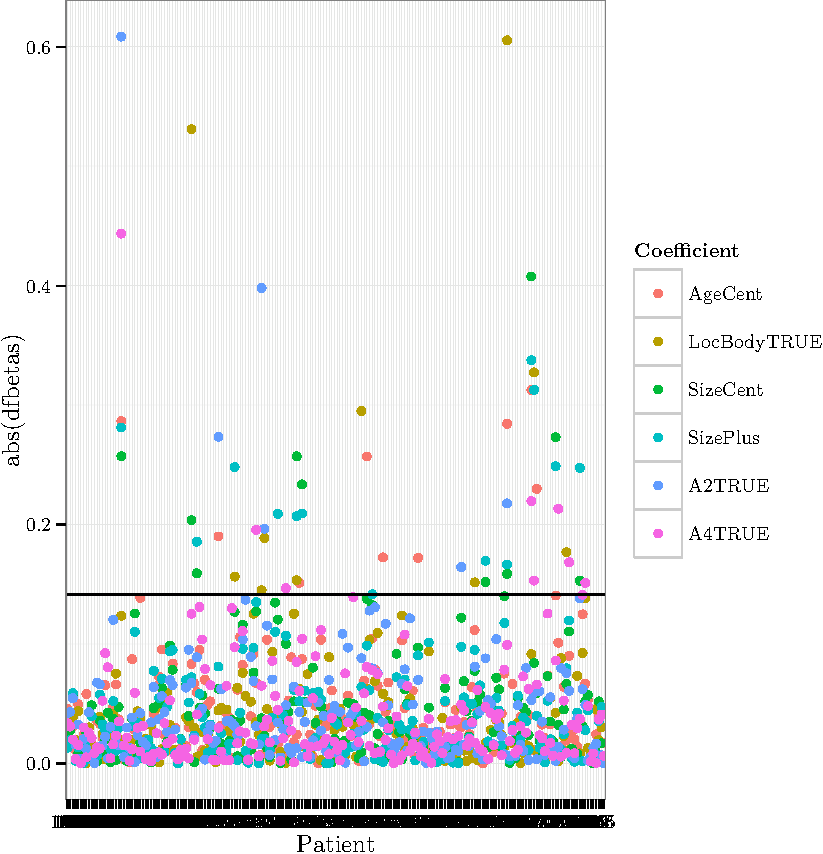
\includegraphics[width=\maxwidth]{figure/05-eda-outliers-2} 

}


\begin{kframe}\begin{alltt}
\hlcom{#sort(apply(abs(resid(fit.cph, type = "dfbetas")), 1, max), decreasing = TRUE)}
\hlkwd{sum}\hlstd{(}\hlkwd{apply}\hlstd{(}\hlkwd{abs}\hlstd{(}\hlkwd{resid}\hlstd{(fit.cph,} \hlkwc{type} \hlstd{=} \hlstr{"dfbetas"}\hlstd{)),} \hlnum{1}\hlstd{, max)} \hlopt{>} \hlnum{2}\hlopt{/}\hlkwd{sqrt}\hlstd{(}\hlkwd{nrow}\hlstd{(data)))}
\end{alltt}
\begin{verbatim}
## [1] 31
\end{verbatim}
\begin{alltt}
\hlstd{temp} \hlkwb{=} \hlkwd{resid}\hlstd{(fit.cph,} \hlkwc{type} \hlstd{=} \hlstr{"dfbetas"}\hlstd{)}
\hlstd{data}\hlopt{$}\hlstd{DFBETAS_max} \hlkwb{=} \hlkwd{apply}\hlstd{(}\hlkwd{abs}\hlstd{(temp),} \hlnum{1}\hlstd{, max)}
\hlstd{data}\hlopt{$}\hlstd{DFBETAS_vars} \hlkwb{=} \hlkwd{apply}\hlstd{(}\hlkwd{abs}\hlstd{(temp),} \hlnum{1}\hlstd{,} \hlkwa{function}\hlstd{(}\hlkwc{x}\hlstd{)} \hlkwd{paste}\hlstd{(}\hlkwd{attr}\hlstd{(fit.cph}\hlopt{$}\hlstd{terms,} \hlstr{"term.labels"}\hlstd{)[x} \hlopt{>} \hlnum{2}\hlopt{/}\hlkwd{sqrt}\hlstd{(}\hlkwd{nrow}\hlstd{(data))],} \hlkwc{collapse} \hlstd{=} \hlstr{","}\hlstd{))}
\hlstd{temp} \hlkwb{=} \hlstd{data[data}\hlopt{$}\hlstd{DFBETAS_max} \hlopt{>=} \hlnum{2}\hlopt{/}\hlkwd{sqrt}\hlstd{(}\hlkwd{nrow}\hlstd{(data))} \hlopt{|} \hlkwd{abs}\hlstd{(data}\hlopt{$}\hlstd{devresid)} \hlopt{>=} \hlnum{2}\hlstd{,]}
\hlcom{#temp[order(temp$DFBETAS_max),]}
\end{alltt}
\end{kframe}
\end{knitrout}

Remove points with deviance residuals > 2.5, or DFBETAS > 0.3.
\begin{knitrout}
\definecolor{shadecolor}{rgb}{0.969, 0.969, 0.969}\color{fgcolor}\begin{kframe}
\begin{alltt}
\hlkwd{nrow}\hlstd{(data)}
\end{alltt}
\begin{verbatim}
## [1] 200
\end{verbatim}
\begin{alltt}
\hlstd{data} \hlkwb{=} \hlstd{data[data}\hlopt{$}\hlstd{DFBETAS_max} \hlopt{<=} \hlnum{0.3} \hlopt{&} \hlkwd{abs}\hlstd{(data}\hlopt{$}\hlstd{devresid)} \hlopt{<=} \hlnum{2.5}\hlstd{,]}
\hlkwd{nrow}\hlstd{(data)}
\end{alltt}
\begin{verbatim}
## [1] 193
\end{verbatim}
\begin{alltt}
\hlstd{fit.cph} \hlkwb{=} \hlkwd{coxph}\hlstd{(}\hlkwd{Surv}\hlstd{(Time, DSD)} \hlopt{~} \hlkwd{strata}\hlstd{(SexM)} \hlopt{+} \hlstd{AgeCent} \hlopt{+} \hlstd{LocBody} \hlopt{+} \hlstd{SizeCent} \hlopt{+} \hlstd{SizePlus} \hlopt{+} \hlstd{A2} \hlopt{+} \hlstd{A4,} \hlkwc{data} \hlstd{= data)}
\end{alltt}
\end{kframe}
\end{knitrout}


\subsection{EDA: Variable selection}
\begin{knitrout}
\definecolor{shadecolor}{rgb}{0.969, 0.969, 0.969}\color{fgcolor}\begin{kframe}
\begin{alltt}
\hlstd{nobs.coxph} \hlkwb{<<-} \hlkwa{function}\hlstd{(}\hlkwc{obj}\hlstd{,} \hlkwc{...}\hlstd{)} \hlkwd{sum}\hlstd{(obj}\hlopt{$}\hlstd{y[,}\hlnum{2}\hlstd{])}
\hlstd{fit.cph.as.bic1} \hlkwb{=} \hlkwd{glmulti}\hlstd{(}\hlkwd{Surv}\hlstd{(Time, DSD)} \hlopt{~} \hlkwd{strata}\hlstd{(SexM)} \hlopt{+} \hlstd{AgeCent} \hlopt{+} \hlstd{LocBody} \hlopt{+} \hlstd{SizeCent} \hlopt{+} \hlstd{SizePlus} \hlopt{+} \hlstd{A2} \hlopt{+} \hlstd{A4,} \hlkwc{data} \hlstd{= data,} \hlkwc{marginality} \hlstd{=} \hlnum{TRUE}\hlstd{,} \hlkwc{method} \hlstd{=} \hlstr{"h"}\hlstd{,} \hlkwc{fitfunction} \hlstd{=} \hlstr{"coxph"}\hlstd{,} \hlkwc{crit} \hlstd{=} \hlstr{"bic"}\hlstd{,} \hlkwc{level} \hlstd{=} \hlnum{1}\hlstd{,} \hlkwc{plotty} \hlstd{=} \hlnum{FALSE}\hlstd{,} \hlkwc{report} \hlstd{=} \hlnum{TRUE}\hlstd{)}
\end{alltt}
\begin{verbatim}
## Initialization...
## TASK: Exhaustive screening of candidate set.
## Fitting...
## 
## After 50 models:
## Best model: Surv(Time,DSD)~1+A2+A4
## Crit= 1569.99720157408
## Mean crit= 1579.04206453807
## 
## After 100 models:
## Best model: Surv(Time,DSD)~1+strata(SexM)+SizeCent+A2
## Crit= 1322.28966392719
## Mean crit= 1493.81514417481
## 
## After 150 models:
## Best model: Surv(Time,DSD)~1+strata(SexM)+SizeCent+A2+A4
## Crit= 1319.12027767861
## Mean crit= 1416.9645603344
## Completed.
\end{verbatim}
\begin{alltt}
\hlstd{fit.cph.as.aicc1} \hlkwb{=} \hlkwd{glmulti}\hlstd{(}\hlkwd{Surv}\hlstd{(Time, DSD)} \hlopt{~} \hlkwd{strata}\hlstd{(SexM)} \hlopt{+} \hlstd{AgeCent} \hlopt{+} \hlstd{LocBody} \hlopt{+} \hlstd{SizeCent} \hlopt{+} \hlstd{SizePlus} \hlopt{+} \hlstd{A2} \hlopt{+} \hlstd{A4,} \hlkwc{data} \hlstd{= data,} \hlkwc{marginality} \hlstd{=} \hlnum{TRUE}\hlstd{,} \hlkwc{method} \hlstd{=} \hlstr{"h"}\hlstd{,} \hlkwc{fitfunction} \hlstd{=} \hlstr{"coxph"}\hlstd{,} \hlkwc{crit} \hlstd{=} \hlstr{"aicc"}\hlstd{,} \hlkwc{level} \hlstd{=} \hlnum{1}\hlstd{,} \hlkwc{plotty} \hlstd{=} \hlnum{FALSE}\hlstd{,} \hlkwc{report} \hlstd{=} \hlnum{TRUE}\hlstd{)}
\end{alltt}
\begin{verbatim}
## Initialization...
## TASK: Exhaustive screening of candidate set.
## Fitting...
## 
## After 50 models:
## Best model: Surv(Time,DSD)~1+LocBody+SizeCent+A4
## Crit= 1562.92910743338
## Mean crit= 1570.63396981566
## 
## After 100 models:
## Best model: Surv(Time,DSD)~1+strata(SexM)+LocBody+SizeCent+A2
## Crit= 1315.8613218026
## Mean crit= 1484.90325895394
## 
## After 150 models:
## Best model: Surv(Time,DSD)~1+strata(SexM)+LocBody+SizeCent+A2+A4
## Crit= 1309.03451494962
## Mean crit= 1406.96604818801
## Completed.
\end{verbatim}
\begin{alltt}
\hlkwd{rm}\hlstd{(nobs.coxph)}
\hlkwd{summary}\hlstd{(fit.cph.as.bic1)}\hlopt{$}\hlstd{bestmodel}
\end{alltt}
\begin{verbatim}
## [1] "Surv(Time, DSD) ~ 1 + strata(SexM) + SizeCent + A2 + A4"
\end{verbatim}
\begin{alltt}
\hlkwd{summary}\hlstd{(fit.cph.as.aicc1)}\hlopt{$}\hlstd{bestmodel}
\end{alltt}
\begin{verbatim}
## [1] "Surv(Time, DSD) ~ 1 + strata(SexM) + LocBody + SizeCent + A2 + "
## [2] "    A4"
\end{verbatim}
\end{kframe}
\end{knitrout}

Also run BIC stepwise, because we can.
\begin{knitrout}
\definecolor{shadecolor}{rgb}{0.969, 0.969, 0.969}\color{fgcolor}\begin{kframe}
\begin{alltt}
\hlkwd{stepAIC}\hlstd{(fit.cph,} \hlkwc{k} \hlstd{=} \hlkwd{log}\hlstd{(}\hlkwd{nrow}\hlstd{(data)))}
\end{alltt}
\begin{verbatim}
## Start:  AIC=1330
## Surv(Time, DSD) ~ strata(SexM) + AgeCent + LocBody + SizeCent + 
##     SizePlus + A2 + A4
## 
##            Df  AIC
## - SizePlus  1 1325
## - SizeCent  1 1326
## - AgeCent   1 1327
## - LocBody   1 1328
## <none>        1330
## - A4        1 1333
## - A2        1 1334
## 
## Step:  AIC=1325
## Surv(Time, DSD) ~ strata(SexM) + AgeCent + LocBody + SizeCent + 
##     A2 + A4
## 
##            Df  AIC
## - AgeCent   1 1322
## - LocBody   1 1322
## - SizeCent  1 1324
## <none>        1325
## - A2        1 1329
## - A4        1 1330
## 
## Step:  AIC=1322
## Surv(Time, DSD) ~ strata(SexM) + LocBody + SizeCent + A2 + A4
## 
##            Df  AIC
## - LocBody   1 1319
## - SizeCent  1 1321
## <none>        1322
## - A2        1 1325
## - A4        1 1326
## 
## Step:  AIC=1319
## Surv(Time, DSD) ~ strata(SexM) + SizeCent + A2 + A4
## 
##            Df  AIC
## <none>        1319
## - SizeCent  1 1322
## - A4        1 1322
## - A2        1 1324
## Call:
## coxph(formula = Surv(Time, DSD) ~ strata(SexM) + SizeCent + A2 + 
##     A4, data = data)
## 
## 
##            coef exp(coef) se(coef)    z      p
## SizeCent 0.0159      1.02  0.00543 2.92 0.0035
## A2TRUE   0.7003      2.01  0.20650 3.39 0.0007
## A4TRUE   0.5154      1.67  0.18497 2.79 0.0053
## 
## Likelihood ratio test=34.1  on 3 df, p=1.92e-07  n= 193, number of events= 184
\end{verbatim}
\begin{alltt}
\hlkwd{stepAIC}\hlstd{(fit.cph,} \hlkwc{k} \hlstd{=} \hlnum{2}\hlstd{)}
\end{alltt}
\begin{verbatim}
## Start:  AIC=1311
## Surv(Time, DSD) ~ strata(SexM) + AgeCent + LocBody + SizeCent + 
##     SizePlus + A2 + A4
## 
##            Df  AIC
## - SizePlus  1 1309
## - SizeCent  1 1310
## - AgeCent   1 1311
## <none>        1311
## - LocBody   1 1311
## - A4        1 1317
## - A2        1 1318
## 
## Step:  AIC=1309
## Surv(Time, DSD) ~ strata(SexM) + AgeCent + LocBody + SizeCent + 
##     A2 + A4
## 
##            Df  AIC
## - AgeCent   1 1309
## <none>        1309
## - LocBody   1 1309
## - SizeCent  1 1311
## - A2        1 1316
## - A4        1 1317
## 
## Step:  AIC=1309
## Surv(Time, DSD) ~ strata(SexM) + LocBody + SizeCent + A2 + A4
## 
##            Df  AIC
## <none>        1309
## - LocBody   1 1309
## - SizeCent  1 1311
## - A2        1 1315
## - A4        1 1316
## Call:
## coxph(formula = Surv(Time, DSD) ~ strata(SexM) + LocBody + SizeCent + 
##     A2 + A4, data = data)
## 
## 
##               coef exp(coef) se(coef)    z      p
## LocBodyTRUE 0.3806      1.46   0.2267 1.68 0.0930
## SizeCent    0.0126      1.01   0.0058 2.18 0.0290
## A2TRUE      0.6301      1.88   0.2120 2.97 0.0030
## A4TRUE      0.5312      1.70   0.1850 2.87 0.0041
## 
## Likelihood ratio test=36.7  on 4 df, p=2.04e-07  n= 193, number of events= 184
\end{verbatim}
\end{kframe}
\end{knitrout}

\subsection{Final Fits}
\begin{knitrout}
\definecolor{shadecolor}{rgb}{0.969, 0.969, 0.969}\color{fgcolor}\begin{kframe}
\begin{alltt}
\hlstd{fit.cph.as.bic} \hlkwb{=} \hlkwd{coxph}\hlstd{(}\hlkwd{Surv}\hlstd{(Time, DSD)} \hlopt{~} \hlkwd{strata}\hlstd{(SexM)} \hlopt{+} \hlstd{SizePlus} \hlopt{+} \hlstd{A2} \hlopt{+} \hlstd{A4,} \hlkwc{data} \hlstd{= data)}
\hlkwd{cox.zph}\hlstd{(fit.cph.as.bic)}
\end{alltt}
\begin{verbatim}
##              rho  chisq     p
## SizePlus  0.0212 0.0876 0.767
## A2TRUE    0.0340 0.2136 0.644
## A4TRUE   -0.0808 1.1972 0.274
## GLOBAL        NA 1.3865 0.709
\end{verbatim}
\begin{alltt}
\hlstd{fit.cph.as.aicc} \hlkwb{=} \hlkwd{coxph}\hlstd{(}\hlkwd{Surv}\hlstd{(Time, DSD)} \hlopt{~} \hlkwd{strata}\hlstd{(SexM)}\hlopt{+}\hlstd{AgeCent}\hlopt{+}\hlstd{LocBody}\hlopt{+}\hlstd{SizeCent}\hlopt{+}\hlstd{A2}\hlopt{+}\hlstd{A4}\hlopt{+}\hlstd{SizeCent}\hlopt{:}\hlstd{AgeCent}\hlopt{+}\hlkwd{strata}\hlstd{(SexM)}\hlopt{:}\hlstd{SizeCent,} \hlkwc{data} \hlstd{= data)}
\hlkwd{cox.zph}\hlstd{(fit.cph.as.aicc)}
\end{alltt}
\begin{verbatim}
##                                     rho   chisq      p
## AgeCent                        -0.16098 5.43356 0.0198
## LocBodyTRUE                     0.03967 0.30863 0.5785
## SizeCent                        0.00379 0.00275 0.9581
## A2TRUE                          0.04060 0.34304 0.5581
## A4TRUE                         -0.06803 0.84941 0.3567
## AgeCent:SizeCent                0.03856 0.28388 0.5942
## strata(SexM)SexM=TRUE:SizeCent  0.00853 0.01322 0.9085
## GLOBAL                               NA 7.49932 0.3788
\end{verbatim}
\begin{alltt}
\hlstd{fit.cph.sw.bic} \hlkwb{=} \hlkwd{coxph}\hlstd{(}\hlkwd{Surv}\hlstd{(Time, DSD)} \hlopt{~} \hlkwd{strata}\hlstd{(SexM)} \hlopt{+} \hlstd{SizeCent} \hlopt{+} \hlstd{A2} \hlopt{+} \hlstd{A4,} \hlkwc{data} \hlstd{= data)}
\hlkwd{cox.zph}\hlstd{(fit.cph.sw.bic)}
\end{alltt}
\begin{verbatim}
##              rho  chisq     p
## SizeCent  0.0162 0.0507 0.822
## A2TRUE    0.0312 0.1797 0.672
## A4TRUE   -0.0874 1.4015 0.236
## GLOBAL        NA 1.4878 0.685
\end{verbatim}
\begin{alltt}
\hlstd{fit.cph.sw.aic} \hlkwb{=} \hlkwd{coxph}\hlstd{(}\hlkwd{Surv}\hlstd{(Time, DSD)} \hlopt{~} \hlkwd{strata}\hlstd{(SexM)} \hlopt{+} \hlstd{LocBody} \hlopt{+} \hlstd{SizeCent} \hlopt{+} \hlstd{A2} \hlopt{+} \hlstd{A4,} \hlkwc{data} \hlstd{= data)}
\hlkwd{cox.zph}\hlstd{(fit.cph.sw.aic)}
\end{alltt}
\begin{verbatim}
##                 rho  chisq     p
## LocBodyTRUE  0.0180 0.0592 0.808
## SizeCent     0.0280 0.1465 0.702
## A2TRUE       0.0292 0.1636 0.686
## A4TRUE      -0.0839 1.2904 0.256
## GLOBAL           NA 1.6815 0.794
\end{verbatim}
\begin{alltt}
\hlstd{fit.cph} \hlkwb{=} \hlstd{fit.cph.sw.aic}
\end{alltt}
\end{kframe}
\end{knitrout}


\begin{knitrout}
\definecolor{shadecolor}{rgb}{0.969, 0.969, 0.969}\color{fgcolor}\begin{kframe}
\begin{alltt}
\hlkwd{plot}\hlstd{(}\hlkwd{residuals}\hlstd{(fit.cph,} \hlstr{"deviance"}\hlstd{))}
\end{alltt}
\end{kframe}

{\centering 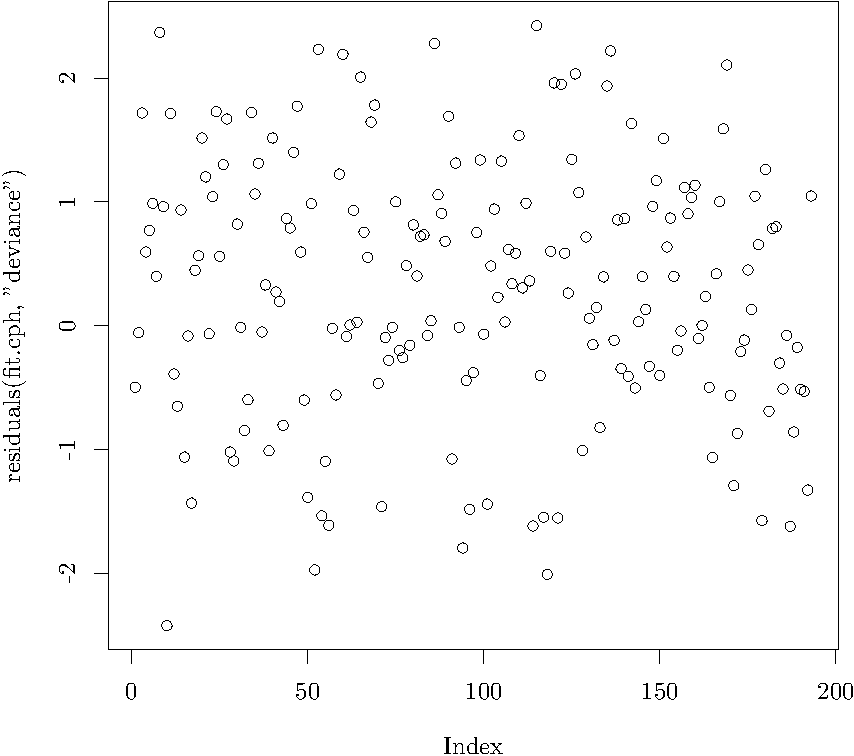
\includegraphics[width=\maxwidth]{figure/05-final-cph-resids-1} 

}


\begin{kframe}\begin{alltt}
\hlkwd{residuals}\hlstd{(fit.cph,} \hlstr{"deviance"}\hlstd{)[}\hlkwd{abs}\hlstd{(}\hlkwd{residuals}\hlstd{(fit.cph,} \hlstr{"deviance"}\hlstd{))} \hlopt{>=} \hlnum{2}\hlstd{]}
\end{alltt}
\begin{verbatim}
##  NSWPCN_125  NSWPCN_133  NSWPCN_315  NSWPCN_324  NSWPCN_333  NSWPCN_374 
##       2.370      -2.425       2.233       2.193       2.009       2.282 
##  NSWPCN_779  NSWPCN_788  NSWPCN_799 NSWPCN_1017 NSWPCN_1165 
##       2.425      -2.011       2.035       2.220       2.107
\end{verbatim}
\begin{alltt}
\hlstd{temp} \hlkwb{=} \hlkwd{sort}\hlstd{(}\hlkwd{apply}\hlstd{(}\hlkwd{abs}\hlstd{(}\hlkwd{residuals}\hlstd{(fit.cph,} \hlstr{"dfbetas"}\hlstd{)),} \hlnum{1}\hlstd{, max))}
\hlcom{#temp}
\hlnum{2}\hlopt{/}\hlkwd{sqrt}\hlstd{(}\hlkwd{nrow}\hlstd{(data))}
\end{alltt}
\begin{verbatim}
## [1] 0.144
\end{verbatim}
\begin{alltt}
\hlkwd{mean}\hlstd{(temp} \hlopt{>} \hlnum{2}\hlopt{/}\hlkwd{sqrt}\hlstd{(}\hlkwd{nrow}\hlstd{(data)))}
\end{alltt}
\begin{verbatim}
## [1] 0.1244
\end{verbatim}
\begin{alltt}
\hlstd{temp[temp} \hlopt{>} \hlnum{2}\hlopt{/}\hlkwd{sqrt}\hlstd{(}\hlkwd{nrow}\hlstd{(data))]}
\end{alltt}
\begin{verbatim}
##  NSWPCN_354  NSWPCN_445  NSWPCN_133  NSWPCN_374  NSWPCN_784  NSWPCN_777 
##      0.1457      0.1524      0.1566      0.1580      0.1618      0.1637 
##  NSWPCN_195  NSWPCN_296  NSWPCN_267 NSWPCN_1155  NSWPCN_154  NSWPCN_794 
##      0.1652      0.1674      0.1711      0.1804      0.1895      0.2037 
##  NSWPCN_802  NSWPCN_142  NSWPCN_799  NSWPCN_313  NSWPCN_192  NSWPCN_317 
##      0.2056      0.2174      0.2178      0.2219      0.2225      0.2541 
##  NSWPCN_318  NSWPCN_788  NSWPCN_145 NSWPCN_1253 NSWPCN_1212  NSWPCN_310 
##      0.2567      0.2749      0.3006      0.4234      0.4528      0.4926
\end{verbatim}
\end{kframe}
\end{knitrout}


\begin{knitrout}
\definecolor{shadecolor}{rgb}{0.969, 0.969, 0.969}\color{fgcolor}\begin{kframe}
\begin{alltt}
\hlkwd{set.seed}\hlstd{(}\hlnum{20150208}\hlstd{)}
\hlstd{fit.rsf} \hlkwb{=} \hlkwd{rfsrc}\hlstd{(}\hlkwd{Surv}\hlstd{(Time, DSD)} \hlopt{~} \hlstd{SexM} \hlopt{+} \hlstd{AgeCent} \hlopt{+} \hlstd{LocBody} \hlopt{+} \hlstd{SizeCent} \hlopt{+} \hlstd{A2} \hlopt{+} \hlstd{A4,} \hlkwc{data} \hlstd{= data,} \hlkwc{mtry} \hlstd{=} \hlnum{1}\hlstd{,} \hlkwc{splitrule} \hlstd{=} \hlstr{"logrankscore"}\hlstd{,} \hlkwc{nsplit} \hlstd{=} \hlnum{2}\hlstd{,} \hlkwc{ntree} \hlstd{=} \hlnum{1000}\hlstd{)}
\hlkwd{plot}\hlstd{(fit.rsf)}
\end{alltt}
\end{kframe}

{\centering 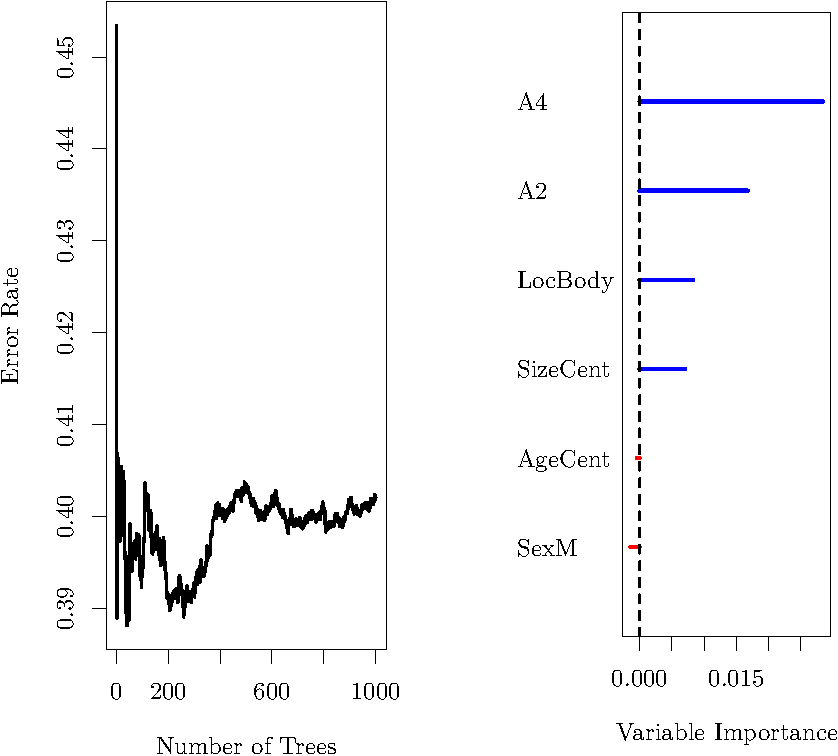
\includegraphics[width=\maxwidth]{figure/05-final-fits-rsf-1} 

}


\begin{kframe}\begin{verbatim}
## 
##            Importance   Relative Imp
## A4             0.0284         1.0000
## A2             0.0167         0.5887
## LocBody        0.0083         0.2920
## SizeCent       0.0071         0.2492
## AgeCent       -0.0004        -0.0149
## SexM          -0.0014        -0.0494
\end{verbatim}
\end{kframe}
\end{knitrout}

\begin{knitrout}
\definecolor{shadecolor}{rgb}{0.969, 0.969, 0.969}\color{fgcolor}\begin{kframe}
\begin{alltt}
\hlstd{fit.gg} \hlkwb{=} \hlkwd{flexsurvreg}\hlstd{(}\hlkwd{Surv}\hlstd{(Time, DSD)} \hlopt{~} \hlstd{SexM} \hlopt{+} \hlstd{LocBody} \hlopt{+} \hlstd{SizeCent} \hlopt{+} \hlstd{A2} \hlopt{+} \hlstd{A4,}
        \hlkwc{anc} \hlstd{=} \hlkwd{list}\hlstd{(}
                \hlkwc{sigma} \hlstd{=} \hlopt{~} \hlstd{SexM,}
                \hlkwc{Q} \hlstd{=} \hlopt{~} \hlstd{SexM),}
        \hlkwc{data} \hlstd{= data,} \hlkwc{dist} \hlstd{=} \hlstr{"gengamma"}\hlstd{)}

\hlstd{fit.gg2} \hlkwb{=} \hlkwd{flexsurvreg}\hlstd{(}\hlkwd{Surv}\hlstd{(Time, DSD)} \hlopt{~} \hlstd{SexM}\hlopt{+}\hlstd{AgeCent}\hlopt{+}\hlstd{LocBody}\hlopt{+}\hlstd{SizeCent}\hlopt{+}\hlstd{A2}\hlopt{+}\hlstd{A4}\hlopt{+}\hlstd{SizeCent}\hlopt{:}\hlstd{AgeCent}\hlopt{+}\hlstd{SexM}\hlopt{:}\hlstd{SizeCent,}
        \hlkwc{anc} \hlstd{=} \hlkwd{list}\hlstd{(}
                \hlkwc{sigma} \hlstd{=} \hlopt{~} \hlstd{SexM,}
                \hlkwc{Q} \hlstd{=} \hlopt{~} \hlstd{SexM),}
        \hlkwc{data} \hlstd{= data,} \hlkwc{dist} \hlstd{=} \hlstr{"gengamma"}\hlstd{)}

\hlstd{fit.gg}\hlopt{$}\hlstd{loglik}
\end{alltt}
\begin{verbatim}
## [1] -1325
\end{verbatim}
\begin{alltt}
\hlstd{fit.gg2}\hlopt{$}\hlstd{loglik}
\end{alltt}
\begin{verbatim}
## [1] -1321
\end{verbatim}
\begin{alltt}
\hlkwd{pchisq}\hlstd{(}\hlnum{2}\hlopt{*}\hlstd{(fit.gg2}\hlopt{$}\hlstd{loglik} \hlopt{-} \hlstd{fit.gg}\hlopt{$}\hlstd{loglik),} \hlnum{3}\hlstd{,} \hlkwc{lower.tail} \hlstd{=} \hlnum{FALSE}\hlstd{)}
\end{alltt}
\begin{verbatim}
## [1] 0.04837
\end{verbatim}
\begin{alltt}
\hlkwd{AIC}\hlstd{(fit.gg)}
\end{alltt}
\begin{verbatim}
## [1] 2669
\end{verbatim}
\begin{alltt}
\hlkwd{AIC}\hlstd{(fit.gg2)}
\end{alltt}
\begin{verbatim}
## [1] 2668
\end{verbatim}
\begin{alltt}
\hlstd{fit.gg}
\end{alltt}
\begin{verbatim}
## 
## Call:
## flexsurvreg(formula = Surv(Time, DSD) ~ SexM + LocBody + SizeCent +     A2 + A4, anc = list(sigma = ~SexM, Q = ~SexM), data = data,     dist = "gengamma")
## 
## Estimates: 
##                  data mean  est       L95%      U95%      se      
## mu                     NA    6.53611   6.19247   6.87976   0.17533
## sigma                  NA    0.78047   0.67245   0.90585   0.05932
## Q                      NA    0.11827  -0.49632   0.73287   0.31357
## SexMTRUE          0.51813    0.28181  -0.07256   0.63619   0.18081
## LocBodyTRUE       0.17098   -0.20952  -0.50577   0.08673   0.15115
## SizeCent          3.65285   -0.00879  -0.01600  -0.00158   0.00368
## A2TRUE            0.16580   -0.38962  -0.65941  -0.11983   0.13765
## A4TRUE            0.75130   -0.39725  -0.62687  -0.16763   0.11716
## sigma(SexMTRUE)   0.51813   -0.26267  -0.49374  -0.03159   0.11790
## Q(SexMTRUE)       0.51813    0.48452  -0.32987   1.29891   0.41551
##                  exp(est)  L95%      U95%    
## mu                     NA        NA        NA
## sigma                  NA        NA        NA
## Q                      NA        NA        NA
## SexMTRUE          1.32553   0.93001   1.88927
## LocBodyTRUE       0.81097   0.60304   1.09060
## SizeCent          0.99124   0.98412   0.99842
## A2TRUE            0.67731   0.51715   0.88707
## A4TRUE            0.67217   0.53426   0.84567
## sigma(SexMTRUE)   0.76900   0.61034   0.96890
## Q(SexMTRUE)       1.62340   0.71902   3.66531
## 
## N = 193,  Events: 184,  Censored: 9
## Total time at risk: 114833
## Log-likelihood = -1325, df = 10
## AIC = 2669
\end{verbatim}
\begin{alltt}
\hlstd{fit.gg2}
\end{alltt}
\begin{verbatim}
## 
## Call:
## flexsurvreg(formula = Surv(Time, DSD) ~ SexM + AgeCent + LocBody +     SizeCent + A2 + A4 + SizeCent:AgeCent + SexM:SizeCent, anc = list(sigma = ~SexM,     Q = ~SexM), data = data, dist = "gengamma")
## 
## Estimates: 
##                    data mean  est        L95%       U95%       se       
## mu                        NA   6.530218   6.184887   6.875549   0.176192
## sigma                     NA   0.771216   0.660311   0.900749   0.061092
## Q                         NA   0.228786  -0.410815   0.868387   0.326333
## SexMTRUE            0.518135   0.322116  -0.039753   0.683986   0.184631
## AgeCent            -1.067358   0.010352   0.000170   0.020534   0.005195
## LocBodyTRUE         0.170984  -0.271326  -0.558764   0.016113   0.146655
## SizeCent            3.652850  -0.004245  -0.015597   0.007107   0.005792
## A2TRUE              0.165803  -0.358631  -0.618603  -0.098660   0.132641
## A4TRUE              0.751295  -0.354054  -0.574822  -0.133287   0.112639
## AgeCent:SizeCent   -8.896373  -0.000855  -0.001550  -0.000160   0.000354
## SexMTRUE:SizeCent   1.772021  -0.006910  -0.020503   0.006684   0.006936
## sigma(SexMTRUE)     0.518135  -0.334045  -0.602093  -0.065998   0.136762
## Q(SexMTRUE)         0.518135   0.550014  -0.328860   1.428889   0.448414
##                    exp(est)   L95%       U95%     
## mu                        NA         NA         NA
## sigma                     NA         NA         NA
## Q                         NA         NA         NA
## SexMTRUE            1.380045   0.961027   1.981761
## AgeCent             1.010406   1.000170   1.020746
## LocBodyTRUE         0.762368   0.571915   1.016243
## SizeCent            0.995764   0.984524   1.007133
## A2TRUE              0.698632   0.538697   0.906051
## A4TRUE              0.701837   0.562805   0.875214
## AgeCent:SizeCent    0.999145   0.998452   0.999840
## SexMTRUE:SizeCent   0.993114   0.979706   1.006706
## sigma(SexMTRUE)     0.716021   0.547664   0.936133
## Q(SexMTRUE)         1.733278   0.719744   4.174059
## 
## N = 193,  Events: 184,  Censored: 9
## Total time at risk: 114833
## Log-likelihood = -1321, df = 13
## AIC = 2668
\end{verbatim}
\end{kframe}
\end{knitrout}

\section{Fit assessment}
Plot fit stratified by sex, separate curves for A2, A4 status, at median (approx.) Size.
\begin{knitrout}
\definecolor{shadecolor}{rgb}{0.969, 0.969, 0.969}\color{fgcolor}\begin{kframe}
\begin{alltt}
\hlstd{temp.grid} \hlkwb{=} \hlkwd{expand.grid}\hlstd{(}\hlkwc{A4} \hlstd{=} \hlkwd{c}\hlstd{(}\hlnum{FALSE}\hlstd{,} \hlnum{TRUE}\hlstd{),} \hlkwc{A2} \hlstd{=} \hlkwd{c}\hlstd{(}\hlnum{FALSE}\hlstd{,} \hlnum{TRUE}\hlstd{),} \hlkwc{SexM} \hlstd{=} \hlkwd{c}\hlstd{(}\hlnum{FALSE}\hlstd{,} \hlnum{TRUE}\hlstd{),} \hlkwc{SizeCent} \hlstd{=} \hlnum{0}\hlstd{,} \hlkwc{AgeCent} \hlstd{=} \hlnum{0}\hlstd{,} \hlkwc{SizePlus} \hlstd{=} \hlnum{0}\hlstd{,} \hlkwc{LocBody} \hlstd{=} \hlkwd{c}\hlstd{(}\hlnum{FALSE}\hlstd{,} \hlnum{TRUE}\hlstd{))}
\hlstd{temp.grid}\hlopt{$}\hlstd{ID} \hlkwb{=} \hlkwd{sprintf}\hlstd{(}\hlstr{"SexM=%s, A2=% -5s, A4=% -5s, LocBody=%s"}\hlstd{, temp.grid}\hlopt{$}\hlstd{SexM, temp.grid}\hlopt{$}\hlstd{A2, temp.grid}\hlopt{$}\hlstd{A4, temp.grid}\hlopt{$}\hlstd{LocBody)}
\hlstd{temp.preds} \hlkwb{=} \hlkwd{summary}\hlstd{(fit.gg,} \hlkwc{newdata} \hlstd{= temp.grid,} \hlkwc{type} \hlstd{=} \hlstr{"survival"}\hlstd{,} \hlkwc{t} \hlstd{=} \hlkwd{seq}\hlstd{(}\hlnum{0}\hlstd{,} \hlnum{365}\hlopt{*}\hlnum{5}\hlstd{,} \hlnum{30}\hlstd{))}
\hlstd{temp.preds2} \hlkwb{=} \hlkwd{do.call}\hlstd{(rbind, temp.preds)}
\hlstd{temp.preds2}\hlopt{$}\hlstd{group} \hlkwb{=} \hlkwd{rep}\hlstd{(}\hlkwd{gsub}\hlstd{(}\hlstr{".*ID="}\hlstd{,} \hlstr{""}\hlstd{,} \hlkwd{names}\hlstd{(temp.preds)),} \hlkwc{each} \hlstd{=} \hlkwd{nrow}\hlstd{(temp.preds[[}\hlnum{1}\hlstd{]]))}
\hlstd{temp.preds.cox} \hlkwb{=} \hlkwd{survfit}\hlstd{(fit.cph,} \hlkwc{newdata} \hlstd{= temp.grid)}
\hlstd{temp.preds.rsf} \hlkwb{=} \hlkwd{predict}\hlstd{(fit.rsf,} \hlkwc{newdata} \hlstd{= temp.grid)}

\hlstd{temp.survfit} \hlkwb{=} \hlkwd{survfit}\hlstd{(}\hlkwd{Surv}\hlstd{(Time, DSD)} \hlopt{~} \hlstd{SexM} \hlopt{+} \hlstd{A2} \hlopt{+} \hlstd{A4} \hlopt{+} \hlstd{LocBody, data)}
\hlstd{temp.data} \hlkwb{=} \hlkwd{data.frame}\hlstd{(}\hlkwc{time} \hlstd{= temp.survfit}\hlopt{$}\hlstd{time}\hlopt{/}\hlnum{365.25}\hlopt{*}\hlnum{12}\hlstd{,} \hlkwc{surv} \hlstd{= temp.survfit}\hlopt{$}\hlstd{surv,} \hlkwc{upper} \hlstd{= temp.survfit}\hlopt{$}\hlstd{lower,} \hlkwc{lower} \hlstd{= temp.survfit}\hlopt{$}\hlstd{upper,} \hlkwc{group} \hlstd{=} \hlkwd{rep}\hlstd{(}\hlkwd{names}\hlstd{(temp.survfit}\hlopt{$}\hlstd{strata), temp.survfit}\hlopt{$}\hlstd{strata),} \hlkwc{Model} \hlstd{=} \hlstr{"KM"}\hlstd{)}
\hlstd{temp.data} \hlkwb{=} \hlkwd{rbind}\hlstd{(temp.data,} \hlkwd{data.frame}\hlstd{(}\hlkwc{time} \hlstd{= temp.preds2}\hlopt{$}\hlstd{time}\hlopt{/}\hlnum{365.25}\hlopt{*}\hlnum{12}\hlstd{,} \hlkwc{surv} \hlstd{= temp.preds2}\hlopt{$}\hlstd{est,} \hlkwc{upper} \hlstd{= temp.preds2}\hlopt{$}\hlstd{ucl,} \hlkwc{lower} \hlstd{= temp.preds2}\hlopt{$}\hlstd{lcl,} \hlkwc{group} \hlstd{= temp.preds2}\hlopt{$}\hlstd{group,} \hlkwc{Model} \hlstd{=} \hlstr{"GG1"}\hlstd{))}
\hlstd{temp.data} \hlkwb{=} \hlkwd{rbind}\hlstd{(temp.data,} \hlkwd{data.frame}\hlstd{(}\hlkwc{time} \hlstd{= temp.preds.cox}\hlopt{$}\hlstd{time}\hlopt{/}\hlnum{365.25}\hlopt{*}\hlnum{12}\hlstd{,} \hlkwc{surv} \hlstd{= temp.preds.cox}\hlopt{$}\hlstd{surv,} \hlkwc{upper} \hlstd{= temp.preds.cox}\hlopt{$}\hlstd{upper,} \hlkwc{lower} \hlstd{= temp.preds.cox}\hlopt{$}\hlstd{lower,} \hlkwc{group} \hlstd{=} \hlkwd{rep}\hlstd{(temp.grid}\hlopt{$}\hlstd{ID, temp.preds.cox}\hlopt{$}\hlstd{strata),} \hlkwc{Model} \hlstd{=} \hlstr{"CP1"}\hlstd{))}
\hlstd{temp.data} \hlkwb{=} \hlkwd{rbind}\hlstd{(temp.data,} \hlkwd{data.frame}\hlstd{(}\hlkwc{time} \hlstd{=} \hlkwd{rep}\hlstd{(temp.preds.rsf}\hlopt{$}\hlstd{time.interest}\hlopt{/}\hlnum{365.25}\hlopt{*}\hlnum{12}\hlstd{,} \hlkwc{each} \hlstd{=} \hlkwd{nrow}\hlstd{(temp.preds.rsf}\hlopt{$}\hlstd{survival)),} \hlkwc{surv} \hlstd{=} \hlkwd{as.vector}\hlstd{(temp.preds.rsf}\hlopt{$}\hlstd{survival),} \hlkwc{upper} \hlstd{=} \hlnum{NA}\hlstd{,} \hlkwc{lower} \hlstd{=} \hlnum{NA}\hlstd{,} \hlkwc{group} \hlstd{=} \hlkwd{rep}\hlstd{(temp.grid}\hlopt{$}\hlstd{ID,} \hlkwd{length}\hlstd{(temp.preds.rsf}\hlopt{$}\hlstd{time.interest)),} \hlkwc{Model} \hlstd{=} \hlstr{"RSF"}\hlstd{))}

\hlstd{temp.data}\hlopt{$}\hlstd{Sex} \hlkwb{=} \hlkwd{c}\hlstd{(}\hlstr{"Male"}\hlstd{,} \hlstr{"Female"}\hlstd{)[}\hlkwd{grepl}\hlstd{(}\hlstr{"SexM=FALSE"}\hlstd{, temp.data}\hlopt{$}\hlstd{group)}\hlopt{+}\hlnum{1}\hlstd{]}
\hlstd{temp.data}\hlopt{$}\hlstd{A2} \hlkwb{=} \hlkwd{c}\hlstd{(}\hlstr{"A2-"}\hlstd{,} \hlstr{"A2+"}\hlstd{)[}\hlkwd{grepl}\hlstd{(}\hlstr{"A2=TRUE"}\hlstd{, temp.data}\hlopt{$}\hlstd{group)}\hlopt{+}\hlnum{1}\hlstd{]}
\hlstd{temp.data}\hlopt{$}\hlstd{A4} \hlkwb{=} \hlkwd{c}\hlstd{(}\hlstr{"A4-"}\hlstd{,} \hlstr{"A4+"}\hlstd{)[}\hlkwd{grepl}\hlstd{(}\hlstr{"A4=TRUE"}\hlstd{, temp.data}\hlopt{$}\hlstd{group)}\hlopt{+}\hlnum{1}\hlstd{]}
\hlstd{temp.data}\hlopt{$}\hlstd{Location} \hlkwb{=} \hlkwd{c}\hlstd{(}\hlstr{"Head"}\hlstd{,} \hlstr{"Body"}\hlstd{)[}\hlkwd{grepl}\hlstd{(}\hlstr{"LocBody=TRUE"}\hlstd{, temp.data}\hlopt{$}\hlstd{group)}\hlopt{+}\hlnum{1}\hlstd{]}

\hlstd{temp.data}\hlopt{$}\hlstd{lower[temp.data}\hlopt{$}\hlstd{model} \hlopt{!=} \hlstr{"KM"}\hlstd{]} \hlkwb{=} \hlnum{NA}
\hlstd{temp.data}\hlopt{$}\hlstd{upper[temp.data}\hlopt{$}\hlstd{model} \hlopt{!=} \hlstr{"KM"}\hlstd{]} \hlkwb{=} \hlnum{NA}
\hlkwd{ggplot}\hlstd{(temp.data,} \hlkwd{aes}\hlstd{(}\hlkwc{x} \hlstd{= time,} \hlkwc{y} \hlstd{= surv,} \hlkwc{ymin} \hlstd{= lower,} \hlkwc{ymax} \hlstd{= upper,} \hlkwc{colour} \hlstd{= Model,} \hlkwc{fill} \hlstd{= Model))} \hlopt{+}
        \hlkwd{geom_ribbon}\hlstd{(}\hlkwc{alpha} \hlstd{=} \hlnum{0.25}\hlstd{,} \hlkwc{colour} \hlstd{=} \hlnum{NA}\hlstd{)} \hlopt{+}
        \hlkwd{geom_line}\hlstd{()} \hlopt{+} \hlkwd{xlim}\hlstd{(}\hlnum{0}\hlstd{,} \hlnum{60}\hlstd{)} \hlopt{+} \hlkwd{ylim}\hlstd{(}\hlnum{0}\hlstd{,} \hlnum{1}\hlstd{)} \hlopt{+} \hlkwd{xlab}\hlstd{(}\hlstr{"Time (months)"}\hlstd{)} \hlopt{+} \hlkwd{ylab}\hlstd{(}\hlstr{"Fraction surviving"}\hlstd{)} \hlopt{+}
        \hlkwd{facet_grid}\hlstd{(A2} \hlopt{~} \hlstd{A4} \hlopt{~} \hlstd{Sex} \hlopt{~} \hlstd{Location)} \hlopt{+}
    \hlkwd{theme_bw}\hlstd{()}
\end{alltt}


{\ttfamily\noindent\color{warningcolor}{\#\# Warning: Removed 9 rows containing missing values (geom\_path).}}

{\ttfamily\noindent\color{warningcolor}{\#\# Warning: Removed 10 rows containing missing values (geom\_path).}}

{\ttfamily\noindent\color{warningcolor}{\#\# Warning: Removed 7 rows containing missing values (geom\_path).}}

{\ttfamily\noindent\color{warningcolor}{\#\# Warning: Removed 9 rows containing missing values (geom\_path).}}

{\ttfamily\noindent\color{warningcolor}{\#\# Warning: Removed 9 rows containing missing values (geom\_path).}}

{\ttfamily\noindent\color{warningcolor}{\#\# Warning: Removed 12 rows containing missing values (geom\_path).}}

{\ttfamily\noindent\color{warningcolor}{\#\# Warning: Removed 7 rows containing missing values (geom\_path).}}

{\ttfamily\noindent\color{warningcolor}{\#\# Warning: Removed 7 rows containing missing values (geom\_path).}}

{\ttfamily\noindent\color{warningcolor}{\#\# Warning: Removed 9 rows containing missing values (geom\_path).}}

{\ttfamily\noindent\color{warningcolor}{\#\# Warning: Removed 9 rows containing missing values (geom\_path).}}

{\ttfamily\noindent\color{warningcolor}{\#\# Warning: Removed 7 rows containing missing values (geom\_path).}}

{\ttfamily\noindent\color{warningcolor}{\#\# Warning: Removed 7 rows containing missing values (geom\_path).}}

{\ttfamily\noindent\color{warningcolor}{\#\# Warning: Removed 9 rows containing missing values (geom\_path).}}

{\ttfamily\noindent\color{warningcolor}{\#\# Warning: Removed 9 rows containing missing values (geom\_path).}}

{\ttfamily\noindent\color{warningcolor}{\#\# Warning: Removed 7 rows containing missing values (geom\_path).}}

{\ttfamily\noindent\color{warningcolor}{\#\# Warning: Removed 7 rows containing missing values (geom\_path).}}\end{kframe}

{\centering 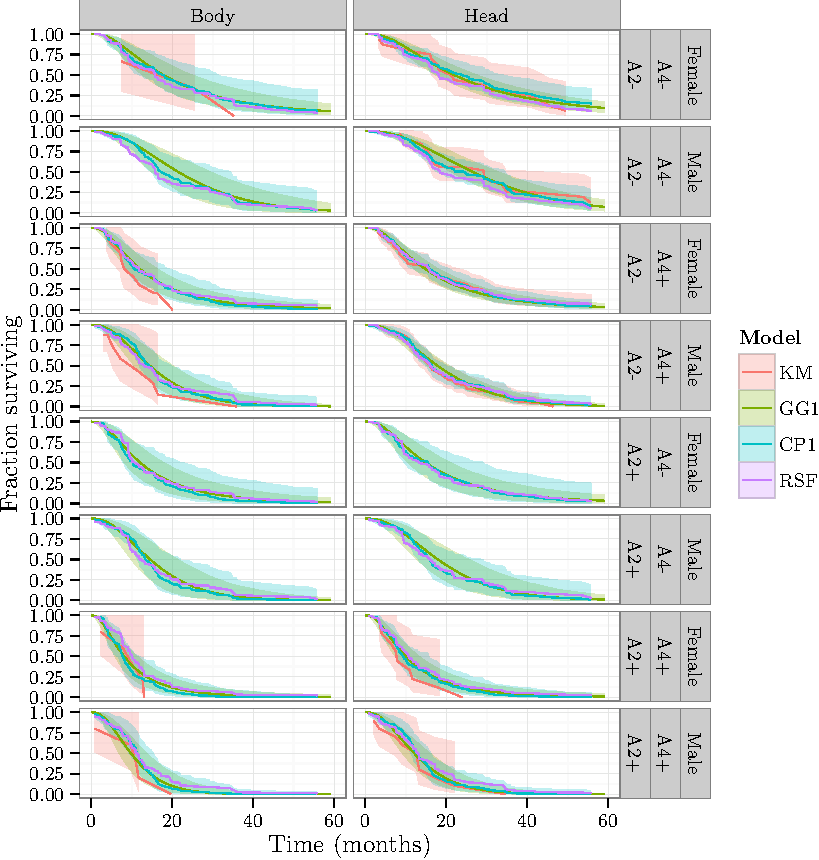
\includegraphics[width=\maxwidth]{figure/05-final-fit-assessment-1} 

}


\begin{kframe}\begin{alltt}
\hlstd{temp.grid} \hlkwb{=} \hlkwd{expand.grid}\hlstd{(}\hlkwc{A4} \hlstd{=} \hlkwd{c}\hlstd{(}\hlnum{FALSE}\hlstd{,} \hlnum{TRUE}\hlstd{),} \hlkwc{A2} \hlstd{=} \hlkwd{c}\hlstd{(}\hlnum{FALSE}\hlstd{,} \hlnum{TRUE}\hlstd{),} \hlkwc{SexM} \hlstd{=} \hlkwd{c}\hlstd{(}\hlnum{FALSE}\hlstd{,} \hlnum{TRUE}\hlstd{),} \hlkwc{SizeCent} \hlstd{=} \hlnum{0}\hlstd{,} \hlkwc{AgeCent} \hlstd{=} \hlnum{0}\hlstd{,} \hlkwc{SizePlus} \hlstd{=} \hlnum{0}\hlstd{,} \hlkwc{LocBody} \hlstd{=} \hlnum{FALSE}\hlstd{)}
\hlstd{temp.grid}\hlopt{$}\hlstd{ID} \hlkwb{=} \hlkwd{sprintf}\hlstd{(}\hlstr{"SexM=%s, A2=% -5s, A4=% -5s, LocBody=%s"}\hlstd{, temp.grid}\hlopt{$}\hlstd{SexM, temp.grid}\hlopt{$}\hlstd{A2, temp.grid}\hlopt{$}\hlstd{A4, temp.grid}\hlopt{$}\hlstd{LocBody)}
\hlstd{temp.preds} \hlkwb{=} \hlkwd{summary}\hlstd{(fit.gg,} \hlkwc{newdata} \hlstd{= temp.grid,} \hlkwc{type} \hlstd{=} \hlstr{"survival"}\hlstd{,} \hlkwc{t} \hlstd{=} \hlkwd{seq}\hlstd{(}\hlnum{0}\hlstd{,} \hlnum{365}\hlopt{*}\hlnum{5}\hlstd{,} \hlnum{30}\hlstd{))}
\hlstd{temp.preds2} \hlkwb{=} \hlkwd{do.call}\hlstd{(rbind, temp.preds)}
\hlstd{temp.preds2}\hlopt{$}\hlstd{group} \hlkwb{=} \hlkwd{rep}\hlstd{(}\hlkwd{gsub}\hlstd{(}\hlstr{".*ID="}\hlstd{,} \hlstr{""}\hlstd{,} \hlkwd{names}\hlstd{(temp.preds)),} \hlkwc{each} \hlstd{=} \hlkwd{nrow}\hlstd{(temp.preds[[}\hlnum{1}\hlstd{]]))}
\hlstd{temp.preds.cox} \hlkwb{=} \hlkwd{survfit}\hlstd{(fit.cph,} \hlkwc{newdata} \hlstd{= temp.grid)}
\hlstd{temp.preds.rsf} \hlkwb{=} \hlkwd{predict}\hlstd{(fit.rsf,} \hlkwc{newdata} \hlstd{= temp.grid)}

\hlstd{temp.survfit} \hlkwb{=} \hlkwd{survfit}\hlstd{(}\hlkwd{Surv}\hlstd{(Time, DSD)} \hlopt{~} \hlstd{SexM} \hlopt{+} \hlstd{A2} \hlopt{+} \hlstd{A4, data)}
\hlstd{temp.data} \hlkwb{=} \hlkwd{data.frame}\hlstd{(}\hlkwc{time} \hlstd{= temp.survfit}\hlopt{$}\hlstd{time}\hlopt{/}\hlnum{365.25}\hlopt{*}\hlnum{12}\hlstd{,} \hlkwc{surv} \hlstd{= temp.survfit}\hlopt{$}\hlstd{surv,} \hlkwc{upper} \hlstd{= temp.survfit}\hlopt{$}\hlstd{lower,} \hlkwc{lower} \hlstd{= temp.survfit}\hlopt{$}\hlstd{upper,} \hlkwc{group} \hlstd{=} \hlkwd{rep}\hlstd{(}\hlkwd{names}\hlstd{(temp.survfit}\hlopt{$}\hlstd{strata), temp.survfit}\hlopt{$}\hlstd{strata),} \hlkwc{Model} \hlstd{=} \hlstr{"KM"}\hlstd{)}
\hlstd{temp.data} \hlkwb{=} \hlkwd{rbind}\hlstd{(temp.data,} \hlkwd{data.frame}\hlstd{(}\hlkwc{time} \hlstd{= temp.preds2}\hlopt{$}\hlstd{time}\hlopt{/}\hlnum{365.25}\hlopt{*}\hlnum{12}\hlstd{,} \hlkwc{surv} \hlstd{= temp.preds2}\hlopt{$}\hlstd{est,} \hlkwc{upper} \hlstd{= temp.preds2}\hlopt{$}\hlstd{ucl,} \hlkwc{lower} \hlstd{= temp.preds2}\hlopt{$}\hlstd{lcl,} \hlkwc{group} \hlstd{= temp.preds2}\hlopt{$}\hlstd{group,} \hlkwc{Model} \hlstd{=} \hlstr{"GG1"}\hlstd{))}
\hlstd{temp.data} \hlkwb{=} \hlkwd{rbind}\hlstd{(temp.data,} \hlkwd{data.frame}\hlstd{(}\hlkwc{time} \hlstd{= temp.preds.cox}\hlopt{$}\hlstd{time}\hlopt{/}\hlnum{365.25}\hlopt{*}\hlnum{12}\hlstd{,} \hlkwc{surv} \hlstd{= temp.preds.cox}\hlopt{$}\hlstd{surv,} \hlkwc{upper} \hlstd{= temp.preds.cox}\hlopt{$}\hlstd{upper,} \hlkwc{lower} \hlstd{= temp.preds.cox}\hlopt{$}\hlstd{lower,} \hlkwc{group} \hlstd{=} \hlkwd{rep}\hlstd{(temp.grid}\hlopt{$}\hlstd{ID, temp.preds.cox}\hlopt{$}\hlstd{strata),} \hlkwc{Model} \hlstd{=} \hlstr{"CP1"}\hlstd{))}
\hlstd{temp.data} \hlkwb{=} \hlkwd{rbind}\hlstd{(temp.data,} \hlkwd{data.frame}\hlstd{(}\hlkwc{time} \hlstd{=} \hlkwd{rep}\hlstd{(temp.preds.rsf}\hlopt{$}\hlstd{time.interest}\hlopt{/}\hlnum{365.25}\hlopt{*}\hlnum{12}\hlstd{,} \hlkwc{each} \hlstd{=} \hlkwd{nrow}\hlstd{(temp.preds.rsf}\hlopt{$}\hlstd{survival)),} \hlkwc{surv} \hlstd{=} \hlkwd{as.vector}\hlstd{(temp.preds.rsf}\hlopt{$}\hlstd{survival),} \hlkwc{upper} \hlstd{=} \hlnum{NA}\hlstd{,} \hlkwc{lower} \hlstd{=} \hlnum{NA}\hlstd{,} \hlkwc{group} \hlstd{=} \hlkwd{rep}\hlstd{(temp.grid}\hlopt{$}\hlstd{ID,} \hlkwd{length}\hlstd{(temp.preds.rsf}\hlopt{$}\hlstd{time.interest)),} \hlkwc{Model} \hlstd{=} \hlstr{"RSF"}\hlstd{))}

\hlstd{temp.data}\hlopt{$}\hlstd{Sex} \hlkwb{=} \hlkwd{c}\hlstd{(}\hlstr{"Male"}\hlstd{,} \hlstr{"Female"}\hlstd{)[}\hlkwd{grepl}\hlstd{(}\hlstr{"SexM=FALSE"}\hlstd{, temp.data}\hlopt{$}\hlstd{group)}\hlopt{+}\hlnum{1}\hlstd{]}
\hlstd{temp.data}\hlopt{$}\hlstd{A2} \hlkwb{=} \hlkwd{c}\hlstd{(}\hlstr{"A2-"}\hlstd{,} \hlstr{"A2+"}\hlstd{)[}\hlkwd{grepl}\hlstd{(}\hlstr{"A2=TRUE"}\hlstd{, temp.data}\hlopt{$}\hlstd{group)}\hlopt{+}\hlnum{1}\hlstd{]}
\hlstd{temp.data}\hlopt{$}\hlstd{A4} \hlkwb{=} \hlkwd{c}\hlstd{(}\hlstr{"A4-"}\hlstd{,} \hlstr{"A4+"}\hlstd{)[}\hlkwd{grepl}\hlstd{(}\hlstr{"A4=TRUE"}\hlstd{, temp.data}\hlopt{$}\hlstd{group)}\hlopt{+}\hlnum{1}\hlstd{]}

\hlstd{temp.data}\hlopt{$}\hlstd{lower[temp.data}\hlopt{$}\hlstd{Model} \hlopt{!=} \hlstr{"KM"}\hlstd{]} \hlkwb{=} \hlnum{NA}
\hlstd{temp.data}\hlopt{$}\hlstd{upper[temp.data}\hlopt{$}\hlstd{Model} \hlopt{!=} \hlstr{"KM"}\hlstd{]} \hlkwb{=} \hlnum{NA}
\hlkwd{ggplot}\hlstd{(temp.data,} \hlkwd{aes}\hlstd{(}\hlkwc{x} \hlstd{= time,} \hlkwc{y} \hlstd{= surv,} \hlkwc{ymin} \hlstd{= lower,} \hlkwc{ymax} \hlstd{= upper,} \hlkwc{colour} \hlstd{= Model,} \hlkwc{fill} \hlstd{= Model))} \hlopt{+}
        \hlkwd{geom_ribbon}\hlstd{(}\hlkwc{alpha} \hlstd{=} \hlnum{0.25}\hlstd{,} \hlkwc{colour} \hlstd{=} \hlnum{NA}\hlstd{)} \hlopt{+}
        \hlkwd{geom_line}\hlstd{()} \hlopt{+} \hlkwd{xlim}\hlstd{(}\hlnum{0}\hlstd{,} \hlnum{60}\hlstd{)} \hlopt{+} \hlkwd{ylim}\hlstd{(}\hlnum{0}\hlstd{,} \hlnum{1}\hlstd{)} \hlopt{+} \hlkwd{xlab}\hlstd{(}\hlstr{"Time (months)"}\hlstd{)} \hlopt{+} \hlkwd{ylab}\hlstd{(}\hlstr{"Fraction surviving"}\hlstd{)} \hlopt{+}
        \hlkwd{facet_grid}\hlstd{(A2} \hlopt{~} \hlstd{A4} \hlopt{~} \hlstd{Sex)} \hlopt{+}
    \hlkwd{theme_bw}\hlstd{()}
\end{alltt}


{\ttfamily\noindent\color{warningcolor}{\#\# Warning: Removed 10 rows containing missing values (geom\_path).}}

{\ttfamily\noindent\color{warningcolor}{\#\# Warning: Removed 9 rows containing missing values (geom\_path).}}

{\ttfamily\noindent\color{warningcolor}{\#\# Warning: Removed 12 rows containing missing values (geom\_path).}}

{\ttfamily\noindent\color{warningcolor}{\#\# Warning: Removed 7 rows containing missing values (geom\_path).}}

{\ttfamily\noindent\color{warningcolor}{\#\# Warning: Removed 9 rows containing missing values (geom\_path).}}

{\ttfamily\noindent\color{warningcolor}{\#\# Warning: Removed 7 rows containing missing values (geom\_path).}}

{\ttfamily\noindent\color{warningcolor}{\#\# Warning: Removed 9 rows containing missing values (geom\_path).}}

{\ttfamily\noindent\color{warningcolor}{\#\# Warning: Removed 7 rows containing missing values (geom\_path).}}\end{kframe}

{\centering 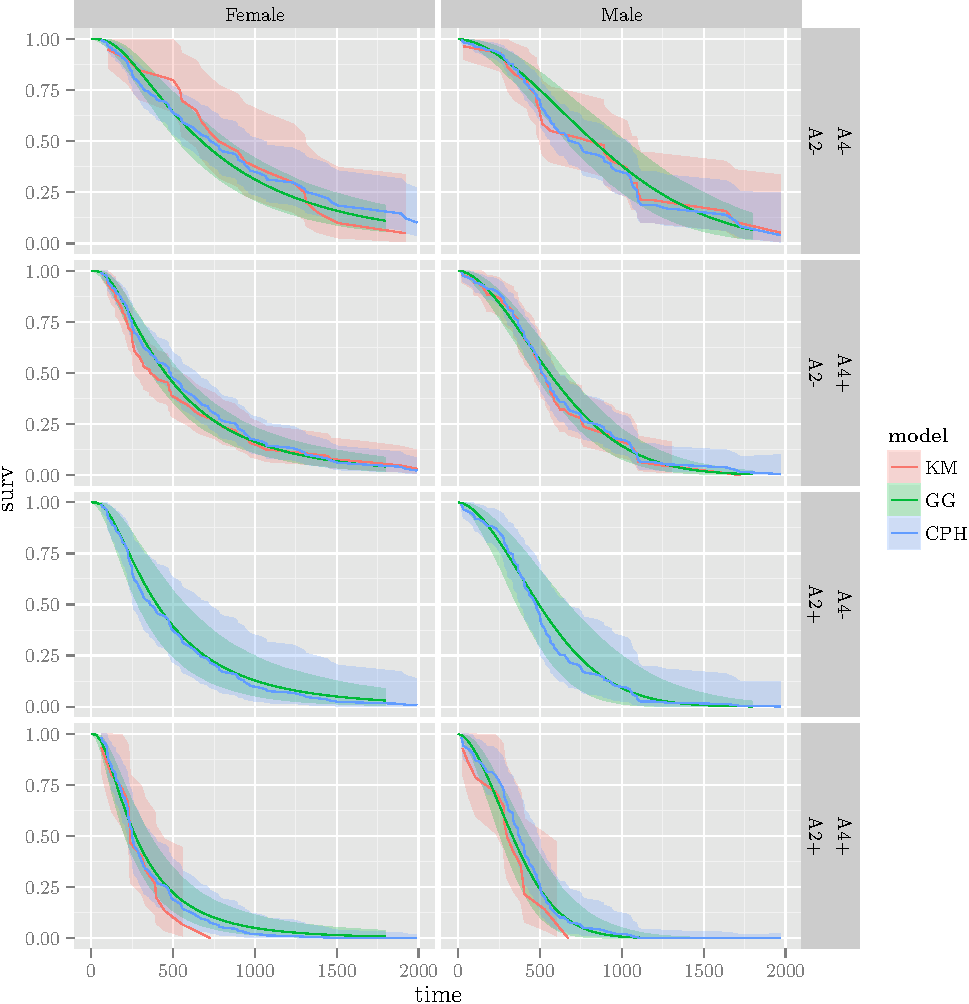
\includegraphics[width=\maxwidth]{figure/05-final-fit-assessment-2} 

}



\end{knitrout}


\section{Model selection}
It looks like that's as far as we can go with tweaking the fits.  Time to put the different models against each other on the holdout data, and choose a winner.

DIY IBS, wooo.
\begin{knitrout}
\definecolor{shadecolor}{rgb}{0.969, 0.969, 0.969}\color{fgcolor}\begin{kframe}
\begin{alltt}
\hlstd{calcIBS} \hlkwb{=} \hlkwa{function}\hlstd{(}\hlkwc{surv}\hlstd{,} \hlkwc{pred}\hlstd{,} \hlkwc{pred_times}\hlstd{,} \hlkwc{max_time}\hlstd{,} \hlkwc{min_time} \hlstd{=} \hlnum{0}\hlstd{)}
\hlstd{\{}
        \hlkwd{stopifnot}\hlstd{(}\hlkwd{nrow}\hlstd{(surv)} \hlopt{==} \hlkwd{nrow}\hlstd{(pred)} \hlopt{&&} \hlkwd{length}\hlstd{(pred_times)} \hlopt{==} \hlkwd{ncol}\hlstd{(pred))}

        \hlstd{n} \hlkwb{=} \hlkwd{nrow}\hlstd{(surv)}
        \hlstd{marg_survfit} \hlkwb{=} \hlkwd{survfit}\hlstd{(surv} \hlopt{~} \hlnum{1}\hlstd{)}
        \hlstd{marg_censfit} \hlkwb{=} \hlkwd{survfit}\hlstd{(}\hlkwd{Surv}\hlstd{(surv[,}\hlnum{1}\hlstd{],} \hlopt{!}\hlstd{surv[,}\hlnum{2}\hlstd{])} \hlopt{~} \hlnum{1}\hlstd{)}
        \hlstd{marg_surv_func} \hlkwb{=} \hlkwd{approxfun}\hlstd{(marg_survfit}\hlopt{$}\hlstd{time, marg_survfit}\hlopt{$}\hlstd{surv,} \hlkwc{method} \hlstd{=} \hlstr{"constant"}\hlstd{,} \hlkwc{yleft} \hlstd{=} \hlnum{1}\hlstd{,} \hlkwc{yright} \hlstd{=} \hlnum{0}\hlstd{,} \hlkwc{rule} \hlstd{=} \hlnum{2}\hlopt{:}\hlnum{1}\hlstd{,} \hlkwc{f} \hlstd{=} \hlnum{0}\hlstd{)}
        \hlstd{marg_cens_func} \hlkwb{=} \hlkwd{approxfun}\hlstd{(marg_censfit}\hlopt{$}\hlstd{time, marg_censfit}\hlopt{$}\hlstd{surv,} \hlkwc{method} \hlstd{=} \hlstr{"constant"}\hlstd{,} \hlkwc{yleft} \hlstd{=} \hlnum{1}\hlstd{,} \hlkwc{yright} \hlstd{=} \hlnum{0}\hlstd{,} \hlkwc{rule} \hlstd{=} \hlnum{2}\hlopt{:}\hlnum{1}\hlstd{,} \hlkwc{f} \hlstd{=} \hlnum{0}\hlstd{)}

        \hlstd{pred_funcs} \hlkwb{=} \hlkwd{apply}\hlstd{(pred,} \hlnum{1}\hlstd{,} \hlkwa{function}\hlstd{(}\hlkwc{pat_preds}\hlstd{)} \hlkwd{approxfun}\hlstd{(pred_times, pat_preds,} \hlkwc{yleft} \hlstd{=} \hlnum{1}\hlstd{,} \hlkwc{yright} \hlstd{=} \hlkwd{min}\hlstd{(pat_preds),} \hlkwc{rule} \hlstd{=} \hlnum{2}\hlstd{))}

        \hlstd{indiv_patient_bsc} \hlkwb{=} \hlkwa{function}\hlstd{(}\hlkwc{pat_i}\hlstd{,} \hlkwc{tstars}\hlstd{)}
        \hlstd{\{}
                \hlstd{observed_time} \hlkwb{=} \hlstd{surv[pat_i,} \hlnum{1}\hlstd{]}
                \hlstd{observed_event} \hlkwb{=} \hlstd{surv[pat_i,} \hlnum{2}\hlstd{]}
                \hlstd{pred_func} \hlkwb{=} \hlstd{pred_funcs[[pat_i]]}
                \hlstd{category} \hlkwb{=} \hlnum{1}\hlopt{*}\hlstd{(observed_time} \hlopt{<=} \hlstd{tstars} \hlopt{&} \hlstd{observed_event)} \hlopt{+} \hlnum{2}\hlopt{*}\hlstd{(observed_time} \hlopt{>} \hlstd{tstars)} \hlopt{+} \hlnum{3}\hlopt{*}\hlstd{(observed_time} \hlopt{<=} \hlstd{tstars} \hlopt{& !}\hlstd{observed_event)}
                \hlstd{bsc} \hlkwb{=} \hlkwd{rep}\hlstd{(}\hlnum{NA}\hlstd{,} \hlkwd{length}\hlstd{(tstars))}
                \hlstd{bsc[category} \hlopt{==} \hlnum{1}\hlstd{]} \hlkwb{=} \hlkwd{pred_func}\hlstd{(tstars[category} \hlopt{==} \hlnum{1}\hlstd{])}\hlopt{^}\hlnum{2} \hlopt{/} \hlkwd{marg_cens_func}\hlstd{(observed_time)}
                \hlstd{bsc[category} \hlopt{==} \hlnum{2}\hlstd{]} \hlkwb{=} \hlstd{(}\hlnum{1} \hlopt{-} \hlkwd{pred_func}\hlstd{(tstars[category} \hlopt{==} \hlnum{2}\hlstd{]))}\hlopt{^}\hlnum{2} \hlopt{/} \hlkwd{marg_cens_func}\hlstd{(tstars[category} \hlopt{==} \hlnum{2}\hlstd{])}
                \hlstd{bsc[category} \hlopt{==} \hlnum{3}\hlstd{]} \hlkwb{=} \hlnum{0}
                \hlstd{bsc}
        \hlstd{\}}

        \hlstd{bsc_func} \hlkwb{=} \hlkwa{function}\hlstd{(}\hlkwc{tstars}\hlstd{) \{} \hlkwd{rowMeans}\hlstd{(}\hlkwd{sapply}\hlstd{(}\hlnum{1}\hlopt{:}\hlstd{n,} \hlkwa{function}\hlstd{(}\hlkwc{pat_i}\hlstd{)} \hlkwd{indiv_patient_bsc}\hlstd{(pat_i, tstars))) \}}

        \hlstd{weight_func} \hlkwb{=} \hlkwa{function}\hlstd{(}\hlkwc{tstars}\hlstd{) \{ (}\hlnum{1} \hlopt{-} \hlkwd{marg_surv_func}\hlstd{(tstars))} \hlopt{/} \hlstd{(}\hlnum{1} \hlopt{-} \hlkwd{marg_surv_func}\hlstd{(max_time)) \}}

        \hlcom{# Be slack and do trapezoidal int. with a fine grid.  It should be possible }
        \hlcom{# to calulate the int. exactly but I cbfed.}
        \hlstd{int_grid} \hlkwb{=} \hlkwd{seq}\hlstd{(min_time, max_time,} \hlkwc{length.out} \hlstd{=} \hlnum{1e3}\hlstd{)}
        \hlstd{bsc_vals} \hlkwb{=} \hlkwd{bsc_func}\hlstd{(int_grid)}
        \hlstd{weight_vals} \hlkwb{=} \hlkwd{weight_func}\hlstd{(int_grid)}
        \hlstd{int_vals} \hlkwb{=} \hlstd{bsc_vals} \hlopt{*} \hlstd{weight_vals}
        \hlstd{ibsc} \hlkwb{=} \hlstd{(}\hlnum{2}\hlopt{*}\hlkwd{sum}\hlstd{(int_vals)} \hlopt{-} \hlstd{int_vals[}\hlnum{1}\hlstd{]} \hlopt{-} \hlstd{int_vals[}\hlkwd{length}\hlstd{(int_vals)])} \hlopt{*} \hlstd{(}\hlkwd{diff}\hlstd{(}\hlkwd{range}\hlstd{(int_grid)))} \hlopt{/} \hlstd{(}\hlnum{2}\hlopt{*}\hlkwd{length}\hlstd{(int_vals))}

        \hlkwd{return}\hlstd{(}\hlkwd{list}\hlstd{(}\hlkwc{bsc} \hlstd{= bsc_vals,} \hlkwc{weights} \hlstd{= weight_vals,} \hlkwc{eval_times} \hlstd{= int_grid,} \hlkwc{ibsc} \hlstd{= ibsc))}
\hlstd{\}}
\end{alltt}
\end{kframe}
\end{knitrout}

Calculate survival probability predictions for each of the models, on the validation data.
\begin{knitrout}
\definecolor{shadecolor}{rgb}{0.969, 0.969, 0.969}\color{fgcolor}\begin{kframe}
\begin{alltt}
\hlstd{ibs_times} \hlkwb{=} \hlkwd{sort}\hlstd{(}\hlkwd{unique}\hlstd{(data.val}\hlopt{$}\hlstd{Time))}
\hlstd{ibs_preds_gg} \hlkwb{=} \hlkwd{as.matrix}\hlstd{(}\hlkwd{t}\hlstd{(}\hlkwd{sapply}\hlstd{(}\hlkwd{summary}\hlstd{(fit.gg,} \hlkwc{newdata} \hlstd{= data.val,} \hlkwc{type} \hlstd{=} \hlstr{"survival"}\hlstd{,} \hlkwc{t} \hlstd{= ibs_times),} \hlkwa{function}\hlstd{(}\hlkwc{x}\hlstd{) x}\hlopt{$}\hlstd{est)))}
\hlstd{ibs_preds_gg2} \hlkwb{=} \hlkwd{as.matrix}\hlstd{(}\hlkwd{t}\hlstd{(}\hlkwd{sapply}\hlstd{(}\hlkwd{summary}\hlstd{(fit.gg2,} \hlkwc{newdata} \hlstd{= data.val,} \hlkwc{type} \hlstd{=} \hlstr{"survival"}\hlstd{,} \hlkwc{t} \hlstd{= ibs_times),} \hlkwa{function}\hlstd{(}\hlkwc{x}\hlstd{) x}\hlopt{$}\hlstd{est)))}
\hlstd{temp_cox_preds} \hlkwb{=} \hlkwd{survfit}\hlstd{(fit.cph,} \hlkwc{newdata} \hlstd{= data.val)}
\hlstd{ibs_preds_cph} \hlkwb{=} \hlkwd{simplify2array}\hlstd{(}\hlkwd{tapply}\hlstd{(}\hlnum{1}\hlopt{:}\hlkwd{length}\hlstd{(temp_cox_preds}\hlopt{$}\hlstd{time),} \hlkwd{rep}\hlstd{(}\hlkwd{names}\hlstd{(temp_cox_preds}\hlopt{$}\hlstd{strata), temp_cox_preds}\hlopt{$}\hlstd{strata),} \hlkwa{function}\hlstd{(}\hlkwc{strat_i}\hlstd{) \{}
        \hlkwd{approx}\hlstd{(}\hlkwc{x} \hlstd{= temp_cox_preds}\hlopt{$}\hlstd{time[strat_i],} \hlkwc{y} \hlstd{= temp_cox_preds}\hlopt{$}\hlstd{surv[strat_i],} \hlkwc{xout} \hlstd{= ibs_times,} \hlkwc{method} \hlstd{=} \hlstr{"constant"}\hlstd{,} \hlkwc{yleft} \hlstd{=} \hlnum{1}\hlstd{,} \hlkwc{rule} \hlstd{=} \hlnum{2}\hlstd{,} \hlkwc{f} \hlstd{=} \hlnum{0}\hlstd{)}\hlopt{$}\hlstd{y \} ))}
\hlstd{ibs_preds_cph} \hlkwb{=} \hlkwd{t}\hlstd{(ibs_preds_cph[,}\hlkwd{rownames}\hlstd{(data.val)])}
\hlstd{temp_rsf_preds} \hlkwb{=} \hlkwd{predict}\hlstd{(fit.rsf,} \hlkwc{newdata} \hlstd{= data.val)}
\hlstd{ibs_preds_rsf} \hlkwb{=} \hlkwd{t}\hlstd{(}\hlkwd{apply}\hlstd{(temp_rsf_preds}\hlopt{$}\hlstd{survival,} \hlnum{1}\hlstd{,} \hlkwa{function}\hlstd{(}\hlkwc{survs}\hlstd{)} \hlkwd{approx}\hlstd{(temp_rsf_preds}\hlopt{$}\hlstd{time.interest, survs,} \hlkwc{xout} \hlstd{= ibs_times,} \hlkwc{method} \hlstd{=} \hlstr{"constant"}\hlstd{,} \hlkwc{yleft} \hlstd{=} \hlnum{1}\hlstd{,} \hlkwc{rule} \hlstd{=} \hlnum{2}\hlstd{,} \hlkwc{f} \hlstd{=} \hlnum{0}\hlstd{)}\hlopt{$}\hlstd{y))}
\hlcom{# Patients (from data.val) are in rows, times (from ibs_times) in columns.}

\hlcom{# Add a no-information KM predictor}
\hlstd{temp_km0} \hlkwb{=} \hlkwd{survfit}\hlstd{(}\hlkwd{Surv}\hlstd{(Time, DSD)} \hlopt{~} \hlnum{1}\hlstd{, data)}
\hlstd{ibs_preds_km0} \hlkwb{=} \hlkwd{t}\hlstd{(}\hlkwd{matrix}\hlstd{(}\hlkwd{rep}\hlstd{(}\hlkwd{approx}\hlstd{(temp_km0}\hlopt{$}\hlstd{time, temp_km0}\hlopt{$}\hlstd{surv,} \hlkwc{xout} \hlstd{= ibs_times,} \hlkwc{method} \hlstd{=} \hlstr{"constant"}\hlstd{,} \hlkwc{yleft} \hlstd{=} \hlnum{1}\hlstd{,} \hlkwc{rule} \hlstd{=} \hlnum{2}\hlstd{,} \hlkwc{f} \hlstd{=} \hlnum{0}\hlstd{)}\hlopt{$}\hlstd{y,} \hlkwc{times} \hlstd{=} \hlkwd{nrow}\hlstd{(data.val)),} \hlkwc{ncol} \hlstd{=} \hlkwd{nrow}\hlstd{(data.val)))}
\hlstd{ibs_preds_all} \hlkwb{=} \hlkwd{list}\hlstd{(}\hlkwc{gg} \hlstd{= ibs_preds_gg,} \hlkwc{gg2} \hlstd{= ibs_preds_gg2,} \hlkwc{cph} \hlstd{= ibs_preds_cph,} \hlkwc{rsf} \hlstd{= ibs_preds_rsf,} \hlkwc{km0} \hlstd{= ibs_preds_km0)}
\end{alltt}
\end{kframe}
\end{knitrout}


\begin{knitrout}
\definecolor{shadecolor}{rgb}{0.969, 0.969, 0.969}\color{fgcolor}\begin{kframe}
\begin{alltt}
\hlstd{val.prob.times} \hlkwb{=} \hlkwd{seq}\hlstd{(}\hlnum{0}\hlstd{,} \hlkwd{max}\hlstd{(data.val}\hlopt{$}\hlstd{Time),} \hlnum{1}\hlstd{)}

\hlstd{temp.coefs} \hlkwb{=} \hlkwd{coef}\hlstd{(fit.gg)}
\hlstd{val.linpred.gg} \hlkwb{=} \hlkwd{sapply}\hlstd{(}\hlnum{1}\hlopt{:}\hlkwd{length}\hlstd{(temp.coefs),} \hlkwa{function}\hlstd{(}\hlkwc{coef_i}\hlstd{) \{}
        \hlcom{# if (names(temp.coefs)[coef_i] == "SexMTRUE") \{}
 \hlcom{#        rep(0, nrow(data.val)) }
        \hlcom{# \} else }
        \hlkwa{if} \hlstd{(}\hlkwd{names}\hlstd{(temp.coefs)[coef_i]} \hlopt \hlkwd{colnames}\hlstd{(data.val)) \{}
        \hlstd{temp.coefs[coef_i]} \hlopt{*} \hlstd{data.val[,}\hlkwd{names}\hlstd{(temp.coefs)[coef_i]]}
    \hlstd{\}} \hlkwa{else if} \hlstd{(}\hlkwd{gsub}\hlstd{(}\hlstr{"TRUE$"}\hlstd{,} \hlstr{""}\hlstd{,} \hlkwd{names}\hlstd{(temp.coefs)[coef_i])} \hlopt \hlkwd{colnames}\hlstd{(data.val)) \{}
        \hlstd{temp.coefs[coef_i]} \hlopt{*} \hlstd{data.val[,}\hlkwd{gsub}\hlstd{(}\hlstr{"TRUE$"}\hlstd{,} \hlstr{""}\hlstd{,} \hlkwd{names}\hlstd{(temp.coefs)[coef_i])]}
    \hlstd{\}} \hlkwa{else} \hlstd{\{}
        \hlkwd{rep}\hlstd{(}\hlnum{0}\hlstd{,} \hlkwd{nrow}\hlstd{(data.val))}
    \hlstd{\} \})}
\hlstd{val.linpred.gg} \hlkwb{=} \hlopt{-}\hlkwd{rowSums}\hlstd{(val.linpred.gg)}   \hlcom{# Negate to bring into concordance with the direction of Cox coefficients (ie higher is now worse)}
\hlstd{temp} \hlkwb{=} \hlkwd{summary}\hlstd{(fit.gg,} \hlkwc{newdata} \hlstd{= data.val,} \hlkwc{ci} \hlstd{=} \hlnum{FALSE}\hlstd{)}
\hlstd{val.prob.gg} \hlkwb{=} \hlkwd{sapply}\hlstd{(temp,} \hlkwa{function}\hlstd{(}\hlkwc{x}\hlstd{)} \hlkwd{approx}\hlstd{(x[,}\hlnum{1}\hlstd{], x[,}\hlnum{2}\hlstd{],} \hlkwc{xout} \hlstd{= val.prob.times,} \hlkwc{yleft} \hlstd{=} \hlnum{1}\hlstd{,} \hlkwc{yright} \hlstd{=} \hlnum{0}\hlstd{,} \hlkwc{rule} \hlstd{=} \hlnum{2}\hlstd{)}\hlopt{$}\hlstd{y)}
\hlkwd{colnames}\hlstd{(val.prob.gg)} \hlkwb{=} \hlkwd{rownames}\hlstd{(data.val)}

\hlstd{temp.coefs} \hlkwb{=} \hlkwd{coef}\hlstd{(fit.gg2)}
\hlstd{val.linpred.gg2} \hlkwb{=} \hlkwd{sapply}\hlstd{(}\hlnum{1}\hlopt{:}\hlkwd{length}\hlstd{(temp.coefs),} \hlkwa{function}\hlstd{(}\hlkwc{coef_i}\hlstd{) \{}
        \hlcom{# if (names(temp.coefs)[coef_i] == "SexMTRUE") \{}
 \hlcom{#        rep(0, nrow(data.val)) }
        \hlcom{# \} else }
        \hlkwa{if} \hlstd{(}\hlkwd{names}\hlstd{(temp.coefs)[coef_i]} \hlopt \hlkwd{colnames}\hlstd{(data.val)) \{}
        \hlstd{temp.coefs[coef_i]} \hlopt{*} \hlstd{data.val[,}\hlkwd{names}\hlstd{(temp.coefs)[coef_i]]}
    \hlstd{\}} \hlkwa{else if} \hlstd{(}\hlkwd{gsub}\hlstd{(}\hlstr{"TRUE$"}\hlstd{,} \hlstr{""}\hlstd{,} \hlkwd{names}\hlstd{(temp.coefs)[coef_i])} \hlopt \hlkwd{colnames}\hlstd{(data.val)) \{}
        \hlstd{temp.coefs[coef_i]} \hlopt{*} \hlstd{data.val[,}\hlkwd{gsub}\hlstd{(}\hlstr{"TRUE$"}\hlstd{,} \hlstr{""}\hlstd{,} \hlkwd{names}\hlstd{(temp.coefs)[coef_i])]}
    \hlstd{\}} \hlkwa{else} \hlstd{\{}
        \hlkwd{rep}\hlstd{(}\hlnum{0}\hlstd{,} \hlkwd{nrow}\hlstd{(data.val))}
    \hlstd{\} \})}
\hlstd{val.linpred.gg2} \hlkwb{=} \hlopt{-}\hlkwd{rowSums}\hlstd{(val.linpred.gg2)}   \hlcom{# Negate to bring into concordance with the direction of Cox coefficients (ie higher is now worse)}
\hlstd{temp} \hlkwb{=} \hlkwd{summary}\hlstd{(fit.gg2,} \hlkwc{newdata} \hlstd{= data.val,} \hlkwc{ci} \hlstd{=} \hlnum{FALSE}\hlstd{)}
\hlstd{val.prob.gg2} \hlkwb{=} \hlkwd{sapply}\hlstd{(temp,} \hlkwa{function}\hlstd{(}\hlkwc{x}\hlstd{)} \hlkwd{approx}\hlstd{(x[,}\hlnum{1}\hlstd{], x[,}\hlnum{2}\hlstd{],} \hlkwc{xout} \hlstd{= val.prob.times,} \hlkwc{yleft} \hlstd{=} \hlnum{1}\hlstd{,} \hlkwc{yright} \hlstd{=} \hlnum{0}\hlstd{,} \hlkwc{rule} \hlstd{=} \hlnum{2}\hlstd{)}\hlopt{$}\hlstd{y)}
\hlkwd{colnames}\hlstd{(val.prob.gg2)} \hlkwb{=} \hlkwd{rownames}\hlstd{(data.val)}

\hlstd{val.linpred.cph} \hlkwb{=} \hlkwd{predict}\hlstd{(fit.cph,} \hlkwc{newdata} \hlstd{= data.val)}
\hlstd{temp} \hlkwb{=} \hlkwd{survfit}\hlstd{(fit.cph,} \hlkwc{newdata} \hlstd{= data.val)}
\hlstd{val.prob.cph} \hlkwb{=} \hlkwd{simplify2array}\hlstd{(}\hlkwd{tapply}\hlstd{(}\hlnum{1}\hlopt{:}\hlkwd{length}\hlstd{(temp}\hlopt{$}\hlstd{surv),} \hlkwd{rep}\hlstd{(}\hlkwd{names}\hlstd{(temp}\hlopt{$}\hlstd{strata), temp}\hlopt{$}\hlstd{strata),} \hlkwa{function}\hlstd{(}\hlkwc{is}\hlstd{)} \hlkwd{approx}\hlstd{(temp}\hlopt{$}\hlstd{time[is], temp}\hlopt{$}\hlstd{surv[is], val.prob.times,} \hlkwc{yleft} \hlstd{=} \hlnum{1}\hlstd{,} \hlkwc{yright} \hlstd{=} \hlnum{0}\hlstd{,} \hlkwc{rule} \hlstd{=} \hlnum{2}\hlstd{)}\hlopt{$}\hlstd{y))[,}\hlkwd{rownames}\hlstd{(data.val)]}

\hlstd{temp} \hlkwb{=} \hlkwd{predict}\hlstd{(fit.rsf,} \hlkwc{newdata} \hlstd{= data.val)}
\hlcom{# val.linpred.rsf = temp$predicted}
\hlcom{# Median survival time:}
\hlstd{val.linpred.rsf} \hlkwb{=} \hlkwd{apply}\hlstd{(temp}\hlopt{$}\hlstd{survival,} \hlnum{1}\hlstd{,} \hlkwa{function}\hlstd{(}\hlkwc{s1}\hlstd{) \{}
    \hlstd{sfunc} \hlkwb{=} \hlkwd{approxfun}\hlstd{(temp}\hlopt{$}\hlstd{time.interest, s1,} \hlkwc{yleft} \hlstd{=} \hlnum{1}\hlstd{,} \hlkwc{yright} \hlstd{=} \hlnum{0}\hlstd{,} \hlkwc{rule} \hlstd{=} \hlnum{2}\hlstd{)}
    \hlstd{med} \hlkwb{=} \hlkwd{uniroot}\hlstd{(}\hlkwa{function}\hlstd{(}\hlkwc{x}\hlstd{)} \hlkwd{sfunc}\hlstd{(x)} \hlopt{-} \hlnum{0.5}\hlstd{,} \hlkwc{lower} \hlstd{=} \hlkwd{min}\hlstd{(temp}\hlopt{$}\hlstd{time.interest),} \hlkwc{upper} \hlstd{=} \hlkwd{max}\hlstd{(temp}\hlopt{$}\hlstd{time.interest))}\hlopt{$}\hlstd{root}
    \hlstd{med}
\hlstd{\})}
\hlstd{val.linpred.rsf} \hlkwb{=} \hlopt{-}\hlstd{val.linpred.rsf}
\hlstd{val.prob.rsf} \hlkwb{=} \hlkwd{apply}\hlstd{(temp}\hlopt{$}\hlstd{survival,} \hlnum{1}\hlstd{,} \hlkwa{function}\hlstd{(}\hlkwc{s1}\hlstd{)} \hlkwd{approx}\hlstd{(temp}\hlopt{$}\hlstd{time.interest, s1,} \hlkwc{xout} \hlstd{= val.prob.times,} \hlkwc{yleft} \hlstd{=} \hlnum{1}\hlstd{,} \hlkwc{yright} \hlstd{=} \hlnum{0}\hlstd{,} \hlkwc{rule} \hlstd{=} \hlnum{2}\hlstd{)}\hlopt{$}\hlstd{y)}
\hlkwd{colnames}\hlstd{(val.prob.rsf)} \hlkwb{=} \hlkwd{rownames}\hlstd{(data.val)}

\hlkwd{summary}\hlstd{(}\hlkwd{coxph}\hlstd{(}\hlkwd{Surv}\hlstd{(Time, DSD)} \hlopt{~} \hlstd{val.linpred.gg, data.val))}
\end{alltt}
\begin{verbatim}
## Call:
## coxph(formula = Surv(Time, DSD) ~ val.linpred.gg, data = data.val)
## 
##   n= 49, number of events= 49 
## 
##                coef exp(coef) se(coef)    z Pr(>|z|)
## val.linpred.gg 1.54      4.68     0.45 3.43    6e-04
## 
##                exp(coef) exp(-coef) lower .95 upper .95
## val.linpred.gg      4.68      0.214      1.94      11.3
## 
## Concordance= 0.673  (se = 0.05 )
## Rsquare= 0.216   (max possible= 0.997 )
## Likelihood ratio test= 11.9  on 1 df,   p=0.000554
## Wald test            = 11.8  on 1 df,   p=0.000599
## Score (logrank) test = 12.2  on 1 df,   p=0.000485
\end{verbatim}
\begin{alltt}
\hlkwd{summary}\hlstd{(}\hlkwd{coxph}\hlstd{(}\hlkwd{Surv}\hlstd{(Time, DSD)} \hlopt{~} \hlstd{val.linpred.gg2, data.val))}
\end{alltt}
\begin{verbatim}
## Call:
## coxph(formula = Surv(Time, DSD) ~ val.linpred.gg2, data = data.val)
## 
##   n= 49, number of events= 49 
## 
##                 coef exp(coef) se(coef)    z Pr(>|z|)
## val.linpred.gg2 1.78      5.93     0.51 3.49  0.00048
## 
##                 exp(coef) exp(-coef) lower .95 upper .95
## val.linpred.gg2      5.93      0.169      2.18      16.1
## 
## Concordance= 0.668  (se = 0.05 )
## Rsquare= 0.216   (max possible= 0.997 )
## Likelihood ratio test= 11.9  on 1 df,   p=0.000563
## Wald test            = 12.2  on 1 df,   p=0.000483
## Score (logrank) test = 12.5  on 1 df,   p=0.00041
\end{verbatim}
\begin{alltt}
\hlkwd{summary}\hlstd{(}\hlkwd{coxph}\hlstd{(}\hlkwd{Surv}\hlstd{(Time, DSD)} \hlopt{~} \hlstd{val.linpred.cph, data.val))}
\end{alltt}
\begin{verbatim}
## Call:
## coxph(formula = Surv(Time, DSD) ~ val.linpred.cph, data = data.val)
## 
##   n= 49, number of events= 49 
## 
##                  coef exp(coef) se(coef)    z Pr(>|z|)
## val.linpred.cph 1.139     3.123    0.311 3.66  0.00025
## 
##                 exp(coef) exp(-coef) lower .95 upper .95
## val.linpred.cph      3.12       0.32       1.7      5.75
## 
## Concordance= 0.65  (se = 0.05 )
## Rsquare= 0.236   (max possible= 0.997 )
## Likelihood ratio test= 13.2  on 1 df,   p=0.000284
## Wald test            = 13.4  on 1 df,   p=0.000252
## Score (logrank) test = 13.9  on 1 df,   p=0.000192
\end{verbatim}
\begin{alltt}
\hlkwd{summary}\hlstd{(}\hlkwd{coxph}\hlstd{(}\hlkwd{Surv}\hlstd{(Time, DSD)} \hlopt{~} \hlstd{val.linpred.rsf, data.val))}
\end{alltt}
\begin{verbatim}
## Call:
## coxph(formula = Surv(Time, DSD) ~ val.linpred.rsf, data = data.val)
## 
##   n= 49, number of events= 49 
## 
##                    coef exp(coef) se(coef)    z Pr(>|z|)
## val.linpred.rsf 0.00811   1.00814  0.00209 3.87  0.00011
## 
##                 exp(coef) exp(-coef) lower .95 upper .95
## val.linpred.rsf      1.01      0.992         1      1.01
## 
## Concordance= 0.663  (se = 0.05 )
## Rsquare= 0.258   (max possible= 0.997 )
## Likelihood ratio test= 14.6  on 1 df,   p=0.000133
## Wald test            = 15  on 1 df,   p=0.000107
## Score (logrank) test = 15.5  on 1 df,   p=8.4e-05
\end{verbatim}
\begin{alltt}
\hlkwd{anova}\hlstd{(}\hlkwd{coxph}\hlstd{(}\hlkwd{Surv}\hlstd{(Time, DSD)} \hlopt{~} \hlkwd{offset}\hlstd{(val.linpred.gg)} \hlopt{+} \hlstd{val.linpred.gg, data.val))}
\end{alltt}
\begin{verbatim}
## Analysis of Deviance Table
##  Cox model: response is Surv(Time, DSD)
## Terms added sequentially (first to last)
## 
##                loglik Chisq Df Pr(>|Chi|)
## NULL             -139                    
## val.linpred.gg   -139  1.47  1       0.23
\end{verbatim}
\begin{alltt}
\hlkwd{anova}\hlstd{(}\hlkwd{coxph}\hlstd{(}\hlkwd{Surv}\hlstd{(Time, DSD)} \hlopt{~} \hlkwd{offset}\hlstd{(val.linpred.gg2)} \hlopt{+} \hlstd{val.linpred.gg2, data.val))}
\end{alltt}
\begin{verbatim}
## Analysis of Deviance Table
##  Cox model: response is Surv(Time, DSD)
## Terms added sequentially (first to last)
## 
##                 loglik Chisq Df Pr(>|Chi|)
## NULL              -140                    
## val.linpred.gg2   -139  2.32  1       0.13
\end{verbatim}
\begin{alltt}
\hlkwd{anova}\hlstd{(}\hlkwd{coxph}\hlstd{(}\hlkwd{Surv}\hlstd{(Time, DSD)} \hlopt{~} \hlkwd{offset}\hlstd{(val.linpred.cph)} \hlopt{+} \hlstd{val.linpred.cph, data.val))}
\end{alltt}
\begin{verbatim}
## Analysis of Deviance Table
##  Cox model: response is Surv(Time, DSD)
## Terms added sequentially (first to last)
## 
##                 loglik Chisq Df Pr(>|Chi|)
## NULL              -138                    
## val.linpred.cph   -138   0.2  1       0.66
\end{verbatim}
\begin{alltt}
\hlkwd{anova}\hlstd{(}\hlkwd{coxph}\hlstd{(}\hlkwd{Surv}\hlstd{(Time, DSD)} \hlopt{~} \hlkwd{offset}\hlstd{(val.linpred.rsf)} \hlopt{+} \hlstd{val.linpred.rsf, data.val))}
\end{alltt}


{\ttfamily\noindent\color{warningcolor}{\#\# Warning in fitter(X, Y, strats, offset, init, control, weights = weights, : Ran out of iterations and did not converge}}

{\ttfamily\noindent\bfseries\color{errorcolor}{\#\# Error in fitter(X, Y, strats, offset, init, control, weights = weights, : NA/NaN/Inf in foreign function call (arg 6)}}\begin{alltt}
\hlkwd{summary}\hlstd{(}\hlkwd{coxph}\hlstd{(}\hlkwd{Surv}\hlstd{(Time, DSD)} \hlopt{~} \hlkwd{offset}\hlstd{(val.linpred.gg)} \hlopt{+} \hlstd{SexM} \hlopt{+} \hlstd{AgeCent} \hlopt{+} \hlstd{LocBody} \hlopt{+} \hlstd{SizeCent} \hlopt{+} \hlstd{A2} \hlopt{+} \hlstd{A4, data.val))}
\end{alltt}
\begin{verbatim}
## Call:
## coxph(formula = Surv(Time, DSD) ~ offset(val.linpred.gg) + SexM + 
##     AgeCent + LocBody + SizeCent + A2 + A4, data = data.val)
## 
##   n= 49, number of events= 49 
## 
##                 coef exp(coef) se(coef)     z Pr(>|z|)
## SexMTRUE     0.10665   1.11255  0.37675  0.28     0.78
## AgeCent     -0.00735   0.99268  0.02276 -0.32     0.75
## LocBodyTRUE  0.29902   1.34854  0.37945  0.79     0.43
## SizeCent     0.00391   1.00392  0.01002  0.39     0.70
## A2TRUE       0.30761   1.36017  0.49719  0.62     0.54
## A4TRUE       0.27581   1.31760  0.39889  0.69     0.49
## 
##             exp(coef) exp(-coef) lower .95 upper .95
## SexMTRUE        1.113      0.899     0.532      2.33
## AgeCent         0.993      1.007     0.949      1.04
## LocBodyTRUE     1.349      0.742     0.641      2.84
## SizeCent        1.004      0.996     0.984      1.02
## A2TRUE          1.360      0.735     0.513      3.60
## A4TRUE          1.318      0.759     0.603      2.88
## 
## Concordance= 0.672  (se = 0.05 )
## Rsquare= 0.064   (max possible= 0.997 )
## Likelihood ratio test= 3.25  on 6 df,   p=0.777
## Wald test            = 3.3  on 6 df,   p=0.77
## Score (logrank) test = 3.36  on 6 df,   p=0.763
\end{verbatim}
\begin{alltt}
\hlkwd{summary}\hlstd{(}\hlkwd{coxph}\hlstd{(}\hlkwd{Surv}\hlstd{(Time, DSD)} \hlopt{~} \hlkwd{offset}\hlstd{(val.linpred.gg2)} \hlopt{+} \hlstd{SexM} \hlopt{+} \hlstd{AgeCent} \hlopt{+} \hlstd{LocBody} \hlopt{+} \hlstd{SizeCent} \hlopt{+} \hlstd{A2} \hlopt{+} \hlstd{A4, data.val))}
\end{alltt}
\begin{verbatim}
## Call:
## coxph(formula = Surv(Time, DSD) ~ offset(val.linpred.gg2) + SexM + 
##     AgeCent + LocBody + SizeCent + A2 + A4, data = data.val)
## 
##   n= 49, number of events= 49 
## 
##                coef exp(coef) se(coef)    z Pr(>|z|)
## SexMTRUE    0.14695   1.15830  0.37675 0.39     0.70
## AgeCent     0.00300   1.00301  0.02276 0.13     0.90
## LocBodyTRUE 0.23722   1.26772  0.37945 0.63     0.53
## SizeCent    0.00846   1.00849  0.01002 0.84     0.40
## A2TRUE      0.33860   1.40298  0.49719 0.68     0.50
## A4TRUE      0.31901   1.37576  0.39889 0.80     0.42
## 
##             exp(coef) exp(-coef) lower .95 upper .95
## SexMTRUE         1.16      0.863     0.554      2.42
## AgeCent          1.00      0.997     0.959      1.05
## LocBodyTRUE      1.27      0.789     0.603      2.67
## SizeCent         1.01      0.992     0.989      1.03
## A2TRUE           1.40      0.713     0.529      3.72
## A4TRUE           1.38      0.727     0.630      3.01
## 
## Concordance= 0.672  (se = 0.05 )
## Rsquare= 0.081   (max possible= 0.997 )
## Likelihood ratio test= 4.13  on 6 df,   p=0.659
## Wald test            = 4.14  on 6 df,   p=0.658
## Score (logrank) test = 4.23  on 6 df,   p=0.646
\end{verbatim}
\begin{alltt}
\hlkwd{summary}\hlstd{(}\hlkwd{coxph}\hlstd{(}\hlkwd{Surv}\hlstd{(Time, DSD)} \hlopt{~} \hlkwd{offset}\hlstd{(val.linpred.cph)} \hlopt{+} \hlstd{SexM} \hlopt{+} \hlstd{AgeCent} \hlopt{+} \hlstd{LocBody} \hlopt{+} \hlstd{SizeCent} \hlopt{+} \hlstd{A2} \hlopt{+} \hlstd{A4, data.val))}
\end{alltt}
\begin{verbatim}
## Call:
## coxph(formula = Surv(Time, DSD) ~ offset(val.linpred.cph) + SexM + 
##     AgeCent + LocBody + SizeCent + A2 + A4, data = data.val)
## 
##   n= 49, number of events= 49 
## 
##                  coef exp(coef)  se(coef)     z Pr(>|z|)
## SexMTRUE    -2.37e-01  7.89e-01  3.77e-01 -0.63     0.53
## AgeCent     -7.35e-03  9.93e-01  2.28e-02 -0.32     0.75
## LocBodyTRUE  1.28e-01  1.14e+00  3.79e-01  0.34     0.74
## SizeCent     5.99e-05  1.00e+00  1.00e-02  0.01     1.00
## A2TRUE       6.71e-02  1.07e+00  4.97e-01  0.13     0.89
## A4TRUE       1.42e-01  1.15e+00  3.99e-01  0.36     0.72
## 
##             exp(coef) exp(-coef) lower .95 upper .95
## SexMTRUE        0.789      1.267     0.377      1.65
## AgeCent         0.993      1.007     0.949      1.04
## LocBodyTRUE     1.137      0.880     0.540      2.39
## SizeCent        1.000      1.000     0.981      1.02
## A2TRUE          1.069      0.935     0.404      2.83
## A4TRUE          1.152      0.868     0.527      2.52
## 
## Concordance= 0.672  (se = 0.05 )
## Rsquare= 0.015   (max possible= 0.996 )
## Likelihood ratio test= 0.73  on 6 df,   p=0.994
## Wald test            = 0.72  on 6 df,   p=0.994
## Score (logrank) test = 0.72  on 6 df,   p=0.994
\end{verbatim}
\begin{alltt}
\hlkwd{summary}\hlstd{(}\hlkwd{coxph}\hlstd{(}\hlkwd{Surv}\hlstd{(Time, DSD)} \hlopt{~} \hlkwd{offset}\hlstd{(val.linpred.rsf)} \hlopt{+} \hlstd{SexM} \hlopt{+} \hlstd{AgeCent} \hlopt{+} \hlstd{LocBody} \hlopt{+} \hlstd{SizeCent} \hlopt{+} \hlstd{A2} \hlopt{+} \hlstd{A4, data.val))}
\end{alltt}


{\ttfamily\noindent\color{warningcolor}{\#\# Warning in fitter(X, Y, strats, offset, init, control, weights = weights, : Ran out of iterations and did not converge}}

{\ttfamily\noindent\bfseries\color{errorcolor}{\#\# Error in fitter(X, Y, strats, offset, init, control, weights = weights, : NA/NaN/Inf in foreign function call (arg 6)}}\end{kframe}
\end{knitrout}


Cumulative-dynamic:
\begin{knitrout}
\definecolor{shadecolor}{rgb}{0.969, 0.969, 0.969}\color{fgcolor}\begin{kframe}
\begin{alltt}
\hlstd{temp.times} \hlkwb{=} \hlkwd{seq}\hlstd{(}\hlnum{0.1}\hlstd{,} \hlnum{48}\hlstd{,} \hlnum{0.1}\hlstd{)}
\hlstd{temp.gg} \hlkwb{=} \hlkwd{timeROC}\hlstd{(}\hlkwc{T} \hlstd{= data.val}\hlopt{$}\hlstd{Time}\hlopt{/}\hlnum{365.25}\hlopt{*}\hlnum{12}\hlstd{,} \hlkwc{delta} \hlstd{= data.val}\hlopt{$}\hlstd{DSD}\hlopt{*}\hlnum{1}\hlstd{,} \hlkwc{marker} \hlstd{= val.linpred.gg,} \hlkwc{cause} \hlstd{=} \hlnum{1}\hlstd{,} \hlkwc{times} \hlstd{= temp.times,} \hlkwc{iid} \hlstd{=} \hlnum{FALSE}\hlstd{)}
\hlstd{temp.gg2} \hlkwb{=} \hlkwd{timeROC}\hlstd{(}\hlkwc{T} \hlstd{= data.val}\hlopt{$}\hlstd{Time}\hlopt{/}\hlnum{365.25}\hlopt{*}\hlnum{12}\hlstd{,} \hlkwc{delta} \hlstd{= data.val}\hlopt{$}\hlstd{DSD}\hlopt{*}\hlnum{1}\hlstd{,} \hlkwc{marker} \hlstd{= val.linpred.gg2,} \hlkwc{cause} \hlstd{=} \hlnum{1}\hlstd{,} \hlkwc{times} \hlstd{= temp.times,} \hlkwc{iid} \hlstd{=} \hlnum{FALSE}\hlstd{)}
\hlstd{temp.rsf} \hlkwb{=} \hlkwd{timeROC}\hlstd{(}\hlkwc{T} \hlstd{= data.val}\hlopt{$}\hlstd{Time}\hlopt{/}\hlnum{365.25}\hlopt{*}\hlnum{12}\hlstd{,} \hlkwc{delta} \hlstd{= data.val}\hlopt{$}\hlstd{DSD}\hlopt{*}\hlnum{1}\hlstd{,} \hlkwc{marker} \hlstd{= val.linpred.rsf,} \hlkwc{cause} \hlstd{=} \hlnum{1}\hlstd{,} \hlkwc{times} \hlstd{= temp.times,} \hlkwc{iid} \hlstd{=} \hlnum{FALSE}\hlstd{)}
\hlstd{temp.cph} \hlkwb{=} \hlkwd{timeROC}\hlstd{(}\hlkwc{T} \hlstd{= data.val}\hlopt{$}\hlstd{Time}\hlopt{/}\hlnum{365.25}\hlopt{*}\hlnum{12}\hlstd{,} \hlkwc{delta} \hlstd{= data.val}\hlopt{$}\hlstd{DSD}\hlopt{*}\hlnum{1}\hlstd{,} \hlkwc{marker} \hlstd{= val.linpred.cph,} \hlkwc{cause} \hlstd{=} \hlnum{1}\hlstd{,} \hlkwc{times} \hlstd{= temp.times,} \hlkwc{iid} \hlstd{=} \hlnum{FALSE}\hlstd{)}
\hlkwd{plotAUCcurve}\hlstd{(temp.gg,} \hlkwc{conf.int} \hlstd{=} \hlnum{FALSE}\hlstd{,} \hlkwc{add} \hlstd{=} \hlnum{FALSE}\hlstd{,} \hlkwc{col} \hlstd{= pal[}\hlstr{"GG"}\hlstd{])}
\hlkwd{plotAUCcurve}\hlstd{(temp.rsf,} \hlkwc{conf.int} \hlstd{=} \hlnum{FALSE}\hlstd{,} \hlkwc{add} \hlstd{=} \hlnum{TRUE}\hlstd{,} \hlkwc{col} \hlstd{= pal[}\hlstr{"RSF"}\hlstd{])}
\hlkwd{plotAUCcurve}\hlstd{(temp.cph,} \hlkwc{conf.int} \hlstd{=} \hlnum{FALSE}\hlstd{,} \hlkwc{add} \hlstd{=} \hlnum{TRUE}\hlstd{,} \hlkwc{col} \hlstd{= pal[}\hlstr{"CPH"}\hlstd{])}
\hlkwd{legend}\hlstd{(}\hlstr{"topright"}\hlstd{,} \hlkwc{legend} \hlstd{=} \hlkwd{c}\hlstd{(}\hlstr{"GG"}\hlstd{,} \hlstr{"RSF"}\hlstd{,} \hlstr{"CPH"}\hlstd{),} \hlkwc{col} \hlstd{= pal[}\hlkwd{c}\hlstd{(}\hlstr{"GG"}\hlstd{,} \hlstr{"RSF"}\hlstd{,} \hlstr{"CPH"}\hlstd{)],} \hlkwc{lty} \hlstd{=} \hlstr{"solid"}\hlstd{)}
\hlkwd{abline}\hlstd{(}\hlkwc{v} \hlstd{=} \hlkwd{c}\hlstd{(}\hlnum{7}\hlstd{,} \hlnum{34}\hlstd{))}
\end{alltt}
\end{kframe}

{\centering 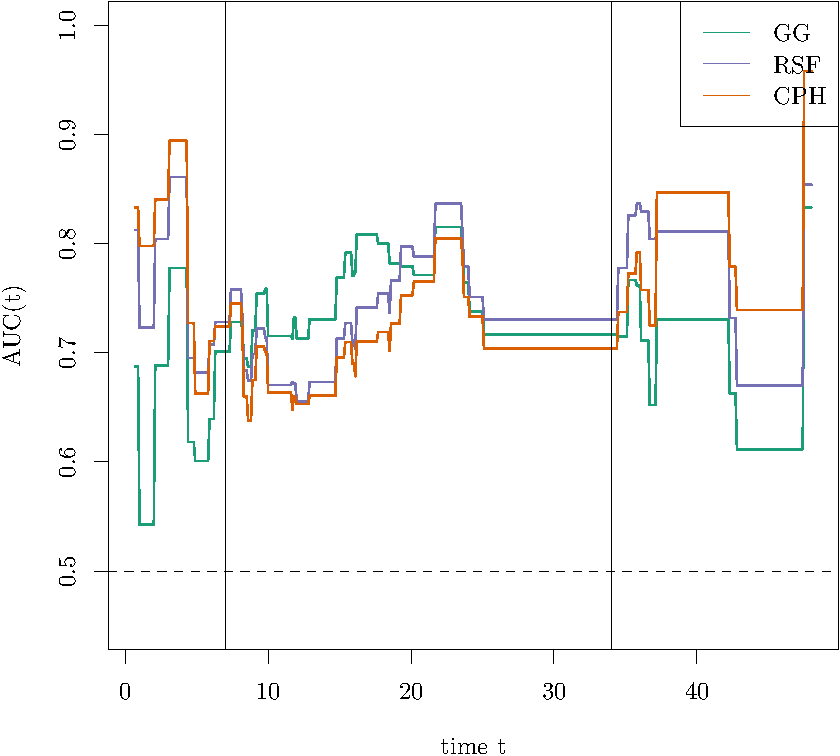
\includegraphics[width=\maxwidth]{figure/05-model-selection-roc-cd-1} 

}


\begin{kframe}\begin{alltt}
\hlkwd{plot}\hlstd{(}\hlkwd{survfit}\hlstd{(}\hlkwd{Surv}\hlstd{(data.val}\hlopt{$}\hlstd{Time}\hlopt{/}\hlnum{365.25}\hlopt{*}\hlnum{12}\hlstd{, data.val}\hlopt{$}\hlstd{DSD)} \hlopt{~} \hlnum{1}\hlstd{))}
\hlkwd{abline}\hlstd{(}\hlkwc{v} \hlstd{=} \hlkwd{c}\hlstd{(}\hlnum{7}\hlstd{,} \hlnum{34}\hlstd{))}
\end{alltt}
\end{kframe}

{\centering 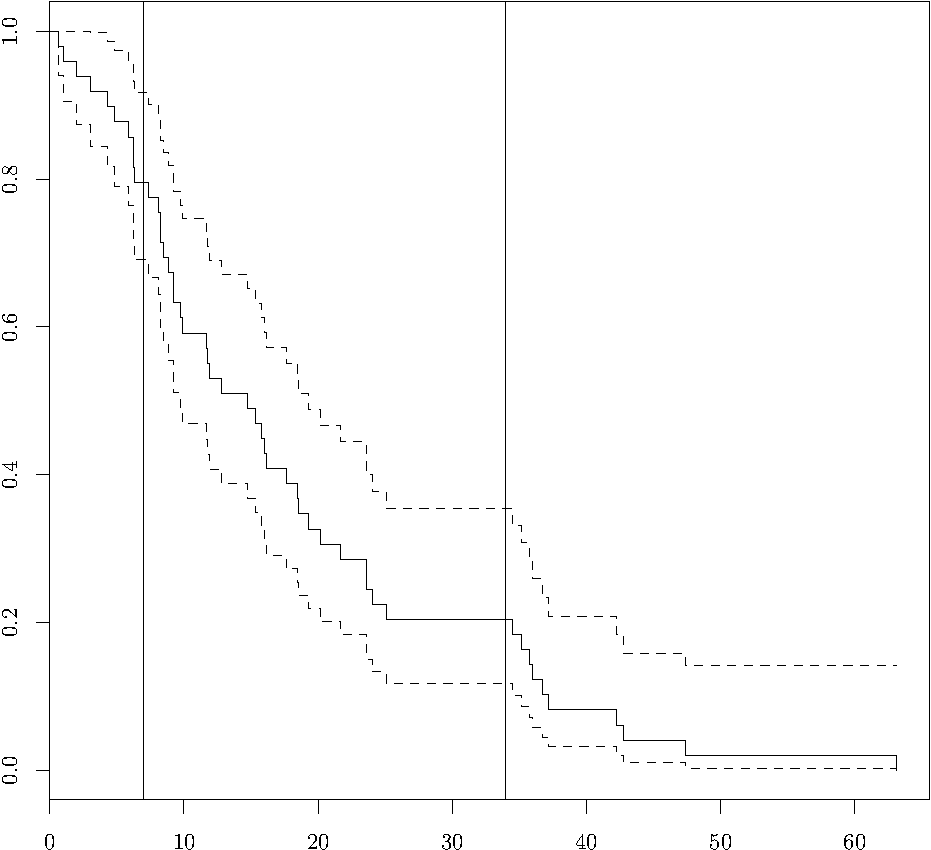
\includegraphics[width=\maxwidth]{figure/05-model-selection-roc-cd-2} 

}



\end{knitrout}


Incident-dynamic:
\begin{knitrout}
\definecolor{shadecolor}{rgb}{0.969, 0.969, 0.969}\color{fgcolor}\begin{kframe}
\begin{alltt}
\hlkwd{library}\hlstd{(risksetROC)}
\hlkwd{invisible}\hlstd{(}\hlkwd{risksetAUC}\hlstd{(data.val}\hlopt{$}\hlstd{Time}\hlopt{/}\hlnum{365.25}\hlopt{*}\hlnum{12}\hlstd{,} \hlkwc{status} \hlstd{= data.val}\hlopt{$}\hlstd{DSD,} \hlkwc{marker} \hlstd{= val.linpred.gg,} \hlkwc{tmax} \hlstd{=} \hlnum{36}\hlstd{,} \hlkwc{col} \hlstd{= pal[}\hlstr{"GG"}\hlstd{],} \hlkwc{lwd} \hlstd{=} \hlnum{2}\hlstd{,} \hlkwc{method} \hlstd{=} \hlstr{"Schoenfeld"}\hlstd{,} \hlkwc{span} \hlstd{=} \hlnum{0.4}\hlstd{))}
\hlkwd{par}\hlstd{(}\hlkwc{new} \hlstd{=} \hlnum{TRUE}\hlstd{)}
\hlkwd{invisible}\hlstd{(}\hlkwd{risksetAUC}\hlstd{(data.val}\hlopt{$}\hlstd{Time}\hlopt{/}\hlnum{365.25}\hlopt{*}\hlnum{12}\hlstd{,} \hlkwc{status} \hlstd{= data.val}\hlopt{$}\hlstd{DSD,} \hlkwc{marker} \hlstd{= val.linpred.rsf,} \hlkwc{tmax} \hlstd{=} \hlnum{36}\hlstd{,} \hlkwc{col} \hlstd{= pal[}\hlstr{"RSF"}\hlstd{],} \hlkwc{lwd} \hlstd{=} \hlnum{2}\hlstd{,} \hlkwc{method} \hlstd{=} \hlstr{"Schoenfeld"}\hlstd{,} \hlkwc{span} \hlstd{=} \hlnum{0.4}\hlstd{))}
\hlkwd{par}\hlstd{(}\hlkwc{new} \hlstd{=} \hlnum{TRUE}\hlstd{)}
\hlkwd{invisible}\hlstd{(}\hlkwd{risksetAUC}\hlstd{(data.val}\hlopt{$}\hlstd{Time}\hlopt{/}\hlnum{365.25}\hlopt{*}\hlnum{12}\hlstd{,} \hlkwc{status} \hlstd{= data.val}\hlopt{$}\hlstd{DSD,} \hlkwc{marker} \hlstd{= val.linpred.cph,} \hlkwc{tmax} \hlstd{=} \hlnum{36}\hlstd{,} \hlkwc{col} \hlstd{= pal[}\hlstr{"CPH"}\hlstd{],} \hlkwc{lwd} \hlstd{=} \hlnum{2}\hlstd{,} \hlkwc{method} \hlstd{=} \hlstr{"Schoenfeld"}\hlstd{,} \hlkwc{span} \hlstd{=} \hlnum{0.4}\hlstd{))}
\hlkwd{par}\hlstd{(}\hlkwc{new} \hlstd{=} \hlnum{TRUE}\hlstd{)}
\hlkwd{legend}\hlstd{(}\hlstr{"top"}\hlstd{,} \hlkwc{legend} \hlstd{=} \hlkwd{c}\hlstd{(}\hlstr{"GG"}\hlstd{,} \hlstr{"RSF"}\hlstd{,} \hlstr{"CPH"}\hlstd{),} \hlkwc{col} \hlstd{= pal[}\hlkwd{c}\hlstd{(}\hlstr{"GG"}\hlstd{,} \hlstr{"RSF"}\hlstd{,} \hlstr{"CPH"}\hlstd{)],} \hlkwc{lty} \hlstd{=} \hlstr{"solid"}\hlstd{)}
\hlkwd{abline}\hlstd{(}\hlkwc{v} \hlstd{=} \hlkwd{c}\hlstd{(}\hlnum{7}\hlstd{,} \hlnum{31}\hlstd{))}
\end{alltt}
\end{kframe}

{\centering 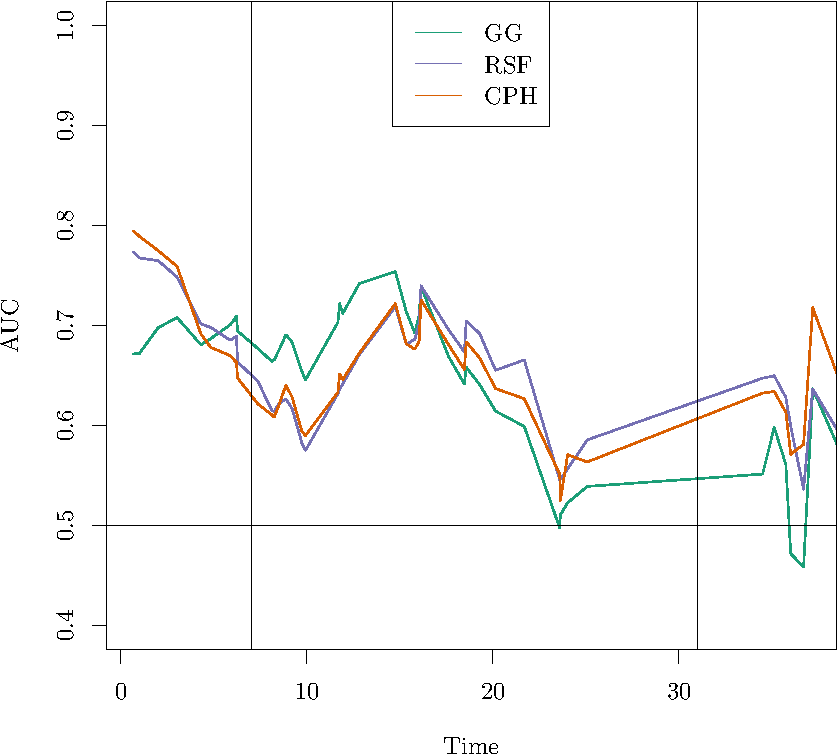
\includegraphics[width=\maxwidth]{figure/05-model-selection-roc-id-1} 

}



\end{knitrout}



Decision curve analysis.
\begin{knitrout}
\definecolor{shadecolor}{rgb}{0.969, 0.969, 0.969}\color{fgcolor}\begin{kframe}
\begin{alltt}
\hlkwd{source}\hlstd{(}\hlstr{"stdca.R"}\hlstd{)}
\hlstd{temp.data} \hlkwb{=} \hlkwd{data.frame}\hlstd{(}\hlkwc{Time} \hlstd{= data.val}\hlopt{$}\hlstd{Time,} \hlkwc{DSD} \hlstd{= data.val}\hlopt{$}\hlstd{DSD}\hlopt{*}\hlnum{1}\hlstd{,}
    \hlkwc{gg.1} \hlstd{=} \hlnum{1}\hlopt{-}\hlstd{val.prob.gg[val.prob.times} \hlopt{==} \hlnum{365}\hlstd{,],} \hlkwc{gg.2} \hlstd{=} \hlnum{1}\hlopt{-}\hlstd{val.prob.gg[val.prob.times} \hlopt{==} \hlnum{365}\hlopt{*}\hlnum{2}\hlstd{,],} \hlkwc{gg.3} \hlstd{=} \hlnum{1}\hlopt{-}\hlstd{val.prob.gg[val.prob.times} \hlopt{==} \hlnum{365}\hlopt{*}\hlnum{3}\hlstd{,],}
    \hlkwc{cph.1} \hlstd{=} \hlnum{1}\hlopt{-}\hlstd{val.prob.cph[val.prob.times} \hlopt{==} \hlnum{365}\hlstd{,],} \hlkwc{cph.2} \hlstd{=} \hlnum{1}\hlopt{-}\hlstd{val.prob.cph[val.prob.times} \hlopt{==} \hlnum{365}\hlopt{*}\hlnum{2}\hlstd{,],} \hlkwc{cph.3} \hlstd{=} \hlnum{1}\hlopt{-}\hlstd{val.prob.cph[val.prob.times} \hlopt{==} \hlnum{365}\hlopt{*}\hlnum{3}\hlstd{,],}
    \hlkwc{rsf.1} \hlstd{=} \hlnum{1}\hlopt{-}\hlstd{val.prob.rsf[val.prob.times} \hlopt{==} \hlnum{365}\hlstd{,],} \hlkwc{rsf.2} \hlstd{=} \hlnum{1}\hlopt{-}\hlstd{val.prob.rsf[val.prob.times} \hlopt{==} \hlnum{365}\hlopt{*}\hlnum{2}\hlstd{,],} \hlkwc{rsf.3} \hlstd{=} \hlnum{1}\hlopt{-}\hlstd{val.prob.rsf[val.prob.times} \hlopt{==} \hlnum{365}\hlopt{*}\hlnum{3}\hlstd{,])}
\hlkwd{invisible}\hlstd{(}\hlkwd{stdca}\hlstd{(}\hlkwc{data} \hlstd{= temp.data,} \hlkwc{outcome} \hlstd{=} \hlstr{"DSD"}\hlstd{,} \hlkwc{ttoutcome} \hlstd{=} \hlstr{"Time"}\hlstd{,} \hlkwc{predictors} \hlstd{=} \hlkwd{c}\hlstd{(}\hlstr{"gg.1"}\hlstd{,} \hlstr{"cph.1"}\hlstd{,} \hlstr{"rsf.1"}\hlstd{),} \hlkwc{timepoint} \hlstd{=} \hlnum{365}\hlstd{,} \hlkwc{probability} \hlstd{=} \hlkwd{rep}\hlstd{(}\hlnum{TRUE}\hlstd{,} \hlnum{3}\hlstd{)))}
\end{alltt}
\begin{verbatim}
## [1] "gg.1: No observations with risk greater than 70% that have followup through the timepoint selected, and therefore net benefit not calculable in this range." 
## [2] "cph.1: No observations with risk greater than 77% that have followup through the timepoint selected, and therefore net benefit not calculable in this range."
## [3] "rsf.1: No observations with risk greater than 64%, and therefore net benefit not calculable in this range."
\end{verbatim}
\end{kframe}

{\centering 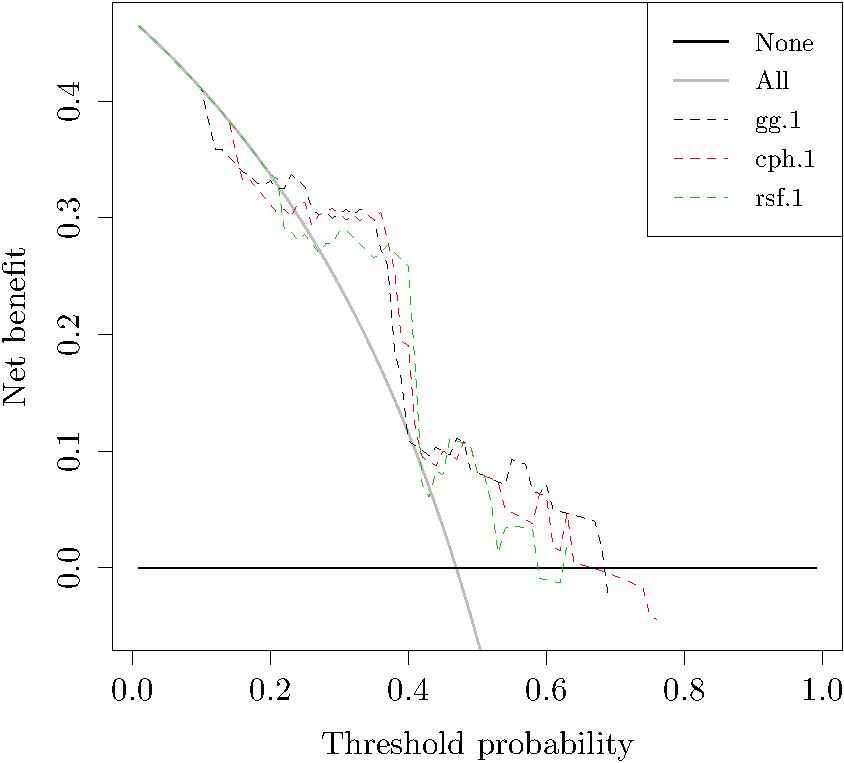
\includegraphics[width=\maxwidth]{figure/05-model-selection-dca-1} 

}


\begin{kframe}\begin{alltt}
\hlkwd{invisible}\hlstd{(}\hlkwd{stdca}\hlstd{(}\hlkwc{data} \hlstd{= temp.data,} \hlkwc{outcome} \hlstd{=} \hlstr{"DSD"}\hlstd{,} \hlkwc{ttoutcome} \hlstd{=} \hlstr{"Time"}\hlstd{,} \hlkwc{predictors} \hlstd{=} \hlkwd{c}\hlstd{(}\hlstr{"gg.2"}\hlstd{,} \hlstr{"cph.2"}\hlstd{,} \hlstr{"rsf.2"}\hlstd{),} \hlkwc{timepoint} \hlstd{=} \hlnum{365}\hlopt{*}\hlnum{2}\hlstd{,} \hlkwc{probability} \hlstd{=} \hlkwd{rep}\hlstd{(}\hlnum{TRUE}\hlstd{,} \hlnum{3}\hlstd{)))}
\end{alltt}
\begin{verbatim}
## [1] "gg.2: No observations with risk greater than 85% that have followup through the timepoint selected, and therefore net benefit not calculable in this range." 
## [2] "cph.2: No observations with risk greater than 83% that have followup through the timepoint selected, and therefore net benefit not calculable in this range."
## [3] "rsf.2: No observations with risk greater than 72% that have followup through the timepoint selected, and therefore net benefit not calculable in this range."
\end{verbatim}
\end{kframe}

{\centering 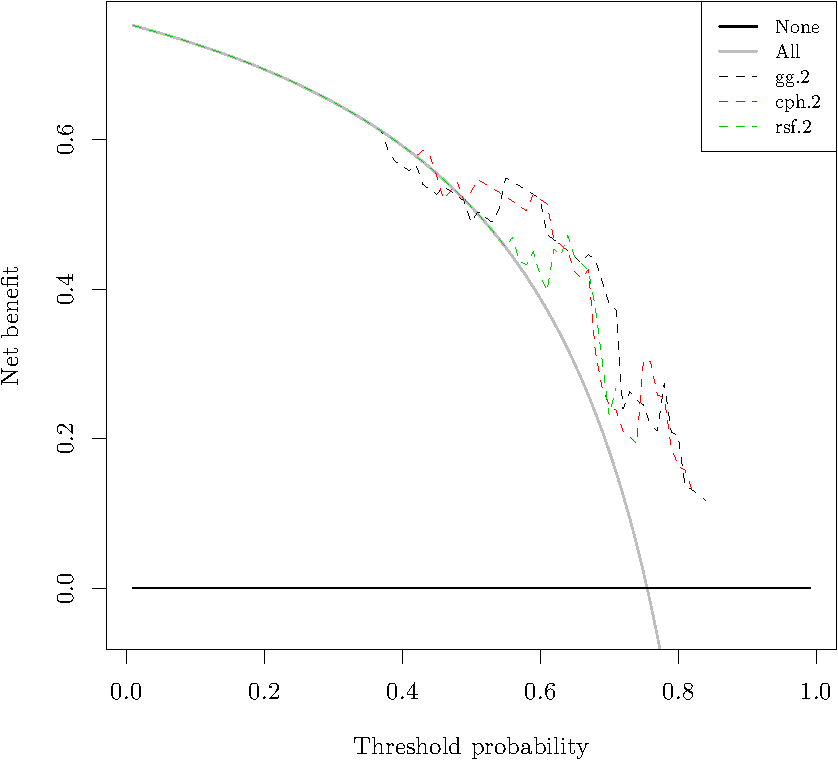
\includegraphics[width=\maxwidth]{figure/05-model-selection-dca-2} 

}


\begin{kframe}\begin{alltt}
\hlkwd{invisible}\hlstd{(}\hlkwd{stdca}\hlstd{(}\hlkwc{data} \hlstd{= temp.data,} \hlkwc{outcome} \hlstd{=} \hlstr{"DSD"}\hlstd{,} \hlkwc{ttoutcome} \hlstd{=} \hlstr{"Time"}\hlstd{,} \hlkwc{predictors} \hlstd{=} \hlkwd{c}\hlstd{(}\hlstr{"gg.3"}\hlstd{,} \hlstr{"cph.3"}\hlstd{,} \hlstr{"rsf.3"}\hlstd{),} \hlkwc{timepoint} \hlstd{=} \hlnum{365}\hlopt{*}\hlnum{3}\hlstd{,} \hlkwc{probability} \hlstd{=} \hlkwd{rep}\hlstd{(}\hlnum{TRUE}\hlstd{,} \hlnum{3}\hlstd{)))}
\end{alltt}
\begin{verbatim}
## [1] "gg.3: No observations with risk greater than 97% that have followup through the timepoint selected, and therefore net benefit not calculable in this range." 
## [2] "cph.3: No observations with risk greater than 97% that have followup through the timepoint selected, and therefore net benefit not calculable in this range."
## [3] "rsf.3: No observations with risk greater than 90% that have followup through the timepoint selected, and therefore net benefit not calculable in this range."
\end{verbatim}
\end{kframe}

{\centering 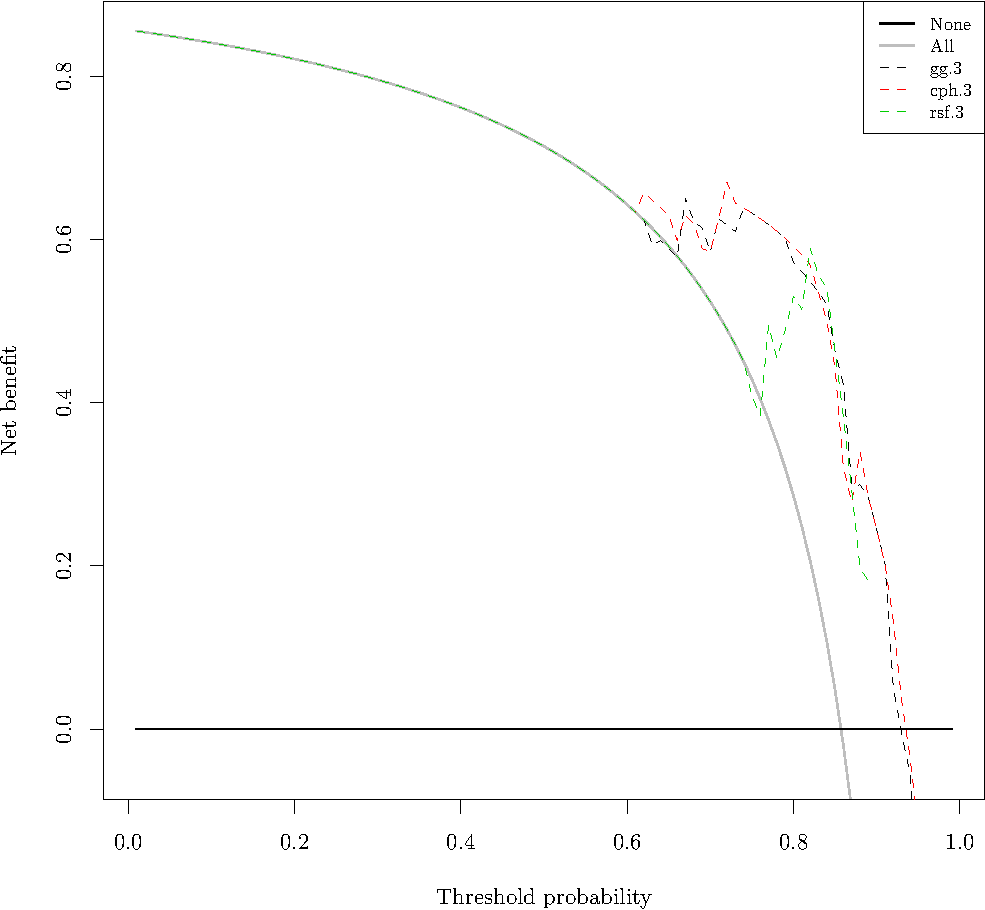
\includegraphics[width=\maxwidth]{figure/05-model-selection-dca-3} 

}



\end{knitrout}


\begin{knitrout}
\definecolor{shadecolor}{rgb}{0.969, 0.969, 0.969}\color{fgcolor}\begin{kframe}
\begin{alltt}
\hlstd{temp} \hlkwb{=} \hlkwd{sapply}\hlstd{(}\hlkwd{list}\hlstd{(}\hlkwc{GG1} \hlstd{= ibs_preds_gg,} \hlkwc{CP1} \hlstd{= ibs_preds_cph,} \hlkwc{RSF} \hlstd{= ibs_preds_rsf,} \hlkwc{KM0} \hlstd{= ibs_preds_km0),} \hlkwa{function}\hlstd{(}\hlkwc{preds}\hlstd{)} \hlkwd{calcIBS}\hlstd{(}\hlkwd{Surv}\hlstd{(data.val}\hlopt{$}\hlstd{Time, data.val}\hlopt{$}\hlstd{DSD), preds, ibs_times,} \hlkwd{max}\hlstd{(data.val}\hlopt{$}\hlstd{Time))}\hlopt{$}\hlstd{bsc)}
\hlstd{temp} \hlkwb{=} \hlkwd{melt}\hlstd{(temp)}
\hlkwd{colnames}\hlstd{(temp)} \hlkwb{=} \hlkwd{c}\hlstd{(}\hlstr{"Time"}\hlstd{,} \hlstr{"Model"}\hlstd{,} \hlstr{"BS"}\hlstd{)}
\hlstd{temp}\hlopt{$}\hlstd{Time} \hlkwb{=} \hlstd{temp}\hlopt{$}\hlstd{Time}\hlopt{/}\hlnum{365.25}\hlopt{*}\hlnum{12}
\hlkwd{ggplot}\hlstd{(temp,} \hlkwd{aes}\hlstd{(}\hlkwc{x} \hlstd{= Time,} \hlkwc{y} \hlstd{= BS,} \hlkwc{colour} \hlstd{= Model))} \hlopt{+} \hlkwd{geom_line}\hlstd{()} \hlopt{+} \hlkwd{ylab}\hlstd{(}\hlstr{"Brier Score"}\hlstd{)} \hlopt{+} \hlkwd{geom_hline}\hlstd{(}\hlkwc{yintercept} \hlstd{=} \hlnum{0.25}\hlstd{)} \hlopt{+} \hlkwd{geom_vline}\hlstd{(}\hlkwc{xintercept} \hlstd{=} \hlkwd{c}\hlstd{(}\hlnum{7}\hlstd{,} \hlnum{34}\hlstd{))} \hlopt{+} \hlkwd{theme_bw}\hlstd{()}
\end{alltt}
\end{kframe}

{\centering 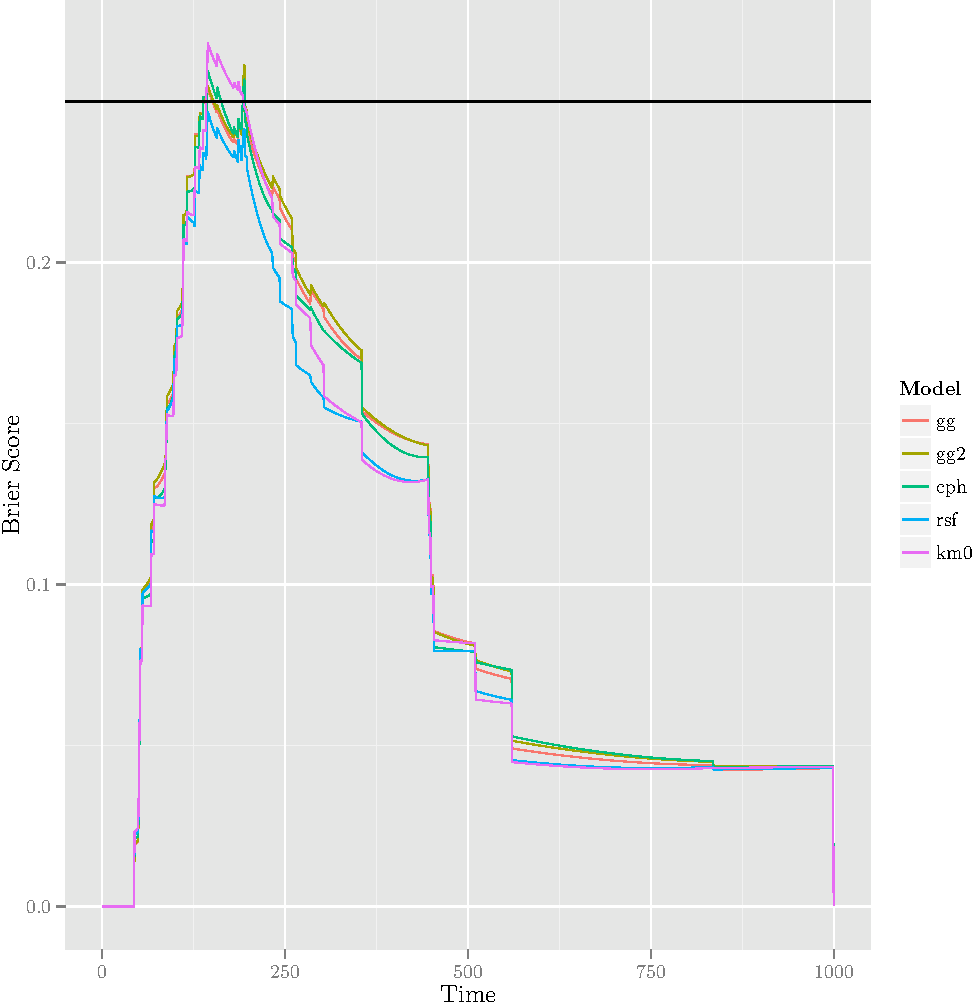
\includegraphics[width=\maxwidth]{figure/05-model-selection-bs-paths-1} 

}



\end{knitrout}

BCA bootstrapping on the differences.
\begin{knitrout}
\definecolor{shadecolor}{rgb}{0.969, 0.969, 0.969}\color{fgcolor}\begin{kframe}
\begin{alltt}
\hlkwd{set.seed}\hlstd{(}\hlnum{20150208}\hlstd{)}
\hlstd{ibsc_boots2} \hlkwb{=} \hlkwd{boot}\hlstd{(data.val,} \hlkwc{statistic} \hlstd{=} \hlkwa{function}\hlstd{(}\hlkwc{d}\hlstd{,} \hlkwc{i}\hlstd{) \{}
        \hlstd{gg} \hlkwb{=} \hlkwd{calcIBS}\hlstd{(}\hlkwd{Surv}\hlstd{(d}\hlopt{$}\hlstd{Time, d}\hlopt{$}\hlstd{DSD)[i,], ibs_preds_gg[i,], ibs_times,} \hlnum{34}\hlopt{*}\hlnum{365.25}\hlopt{/}\hlnum{12}\hlstd{,} \hlnum{7}\hlopt{*}\hlnum{365.25}\hlopt{/}\hlnum{12}\hlstd{)}\hlopt{$}\hlstd{ibs}
        \hlstd{cph} \hlkwb{=} \hlkwd{calcIBS}\hlstd{(}\hlkwd{Surv}\hlstd{(d}\hlopt{$}\hlstd{Time, d}\hlopt{$}\hlstd{DSD)[i,], ibs_preds_cph[i,], ibs_times,} \hlnum{34}\hlopt{*}\hlnum{365.25}\hlopt{/}\hlnum{12}\hlstd{,} \hlnum{7}\hlopt{*}\hlnum{365.25}\hlopt{/}\hlnum{12}\hlstd{)}\hlopt{$}\hlstd{ibs}
        \hlstd{rsf} \hlkwb{=} \hlkwd{calcIBS}\hlstd{(}\hlkwd{Surv}\hlstd{(d}\hlopt{$}\hlstd{Time, d}\hlopt{$}\hlstd{DSD)[i,], ibs_preds_rsf[i,], ibs_times,} \hlnum{34}\hlopt{*}\hlnum{365.25}\hlopt{/}\hlnum{12}\hlstd{,} \hlnum{7}\hlopt{*}\hlnum{365.25}\hlopt{/}\hlnum{12}\hlstd{)}\hlopt{$}\hlstd{ibs}
        \hlstd{km0} \hlkwb{=} \hlkwd{calcIBS}\hlstd{(}\hlkwd{Surv}\hlstd{(d}\hlopt{$}\hlstd{Time, d}\hlopt{$}\hlstd{DSD)[i,], ibs_preds_km0[i,], ibs_times,} \hlnum{34}\hlopt{*}\hlnum{365.25}\hlopt{/}\hlnum{12}\hlstd{,} \hlnum{7}\hlopt{*}\hlnum{365.25}\hlopt{/}\hlnum{12}\hlstd{)}\hlopt{$}\hlstd{ibs}
        \hlkwd{c}\hlstd{(gg} \hlopt{-} \hlstd{km0, cph} \hlopt{-} \hlstd{km0, rsf} \hlopt{-} \hlstd{km0, gg} \hlopt{-} \hlstd{rsf, cph} \hlopt{-} \hlstd{rsf, gg} \hlopt{-} \hlstd{cph)}
\hlstd{\},} \hlkwc{R} \hlstd{=} \hlnum{1000}\hlstd{)}
\hlstd{ibsc_boots2_ci} \hlkwb{=} \hlkwd{t}\hlstd{(}\hlkwd{sapply}\hlstd{(}\hlnum{1}\hlopt{:}\hlkwd{length}\hlstd{(ibsc_boots2}\hlopt{$}\hlstd{t0),} \hlkwa{function}\hlstd{(}\hlkwc{i}\hlstd{)} \hlkwd{boot.ci}\hlstd{(ibsc_boots2,} \hlkwc{index} \hlstd{= i,} \hlkwc{type} \hlstd{=} \hlstr{"bca"}\hlstd{)}\hlopt{$}\hlstd{bca))}
\hlkwd{rownames}\hlstd{(ibsc_boots2_ci)} \hlkwb{=} \hlkwd{c}\hlstd{(}\hlstr{"gg-km0"}\hlstd{,} \hlstr{"cph-km0"}\hlstd{,} \hlstr{"rsf-km0"}\hlstd{,} \hlstr{"gg-rsf"}\hlstd{,} \hlstr{"cph-rsf"}\hlstd{,} \hlstr{"gg-cph"}\hlstd{)}
\hlkwd{colnames}\hlstd{(ibsc_boots2_ci)} \hlkwb{=} \hlkwd{c}\hlstd{(}\hlstr{"level"}\hlstd{,} \hlstr{"orderi1"}\hlstd{,} \hlstr{"orderi2"}\hlstd{,} \hlstr{"lci"}\hlstd{,} \hlstr{"uci"}\hlstd{)}
\hlstd{ibsc_boots2}
\end{alltt}
\begin{verbatim}
## 
## ORDINARY NONPARAMETRIC BOOTSTRAP
## 
## 
## Call:
## boot(data = data.val, statistic = function(d, i) {
##     gg = calcIBS(Surv(d$Time, d$DSD)[i, ], ibs_preds_gg[i, ], 
##         ibs_times, 34 * 365.25/12, 7 * 365.25/12)$ibs
##     cph = calcIBS(Surv(d$Time, d$DSD)[i, ], ibs_preds_cph[i, 
##         ], ibs_times, 34 * 365.25/12, 7 * 365.25/12)$ibs
##     rsf = calcIBS(Surv(d$Time, d$DSD)[i, ], ibs_preds_rsf[i, 
##         ], ibs_times, 34 * 365.25/12, 7 * 365.25/12)$ibs
##     km0 = calcIBS(Surv(d$Time, d$DSD)[i, ], ibs_preds_km0[i, 
##         ], ibs_times, 34 * 365.25/12, 7 * 365.25/12)$ibs
##     c(gg - km0, cph - km0, rsf - km0, gg - rsf, cph - rsf, gg - 
##         cph)
## }, R = 1000)
## 
## 
## Bootstrap Statistics :
##     original  bias    std. error
## t1*  -21.062 0.78762       9.856
## t2*  -20.209 0.72053       9.039
## t3*  -14.505 0.34307       4.952
## t4*   -6.557 0.44455       5.798
## t5*   -5.704 0.37746       4.772
## t6*   -0.853 0.06709       2.123
\end{verbatim}
\begin{alltt}
\hlstd{ibsc_boots2_ci}
\end{alltt}
\begin{verbatim}
##         level orderi1 orderi2     lci    uci
## gg-km0   0.95   19.71   969.3 -39.793 -2.523
## cph-km0  0.95   15.13   961.7 -38.853 -4.508
## rsf-km0  0.95   14.19   960.0 -24.557 -5.655
## gg-rsf   0.95   24.04   974.9 -17.721  5.620
## cph-rsf  0.95   16.32   963.5 -15.865  2.877
## gg-cph   0.95   37.22   985.5  -4.343  4.087
\end{verbatim}
\end{kframe}
\end{knitrout}
All models perform equivalently on the validation set.  Select the simplest: gg.


%%%%%%%%%%%%%%%%%%%%%%%%%%%%%%%%%%%%%%%%%%%%%%%%%%%%%%%%%%%%%%%%%%%%%%
% CALCULATE AND SAVE FINAL MODEL
%%%%%%%%%%%%%%%%%%%%%%%%%%%%%%%%%%%%%%%%%%%%%%%%%%%%%%%%%%%%%%%%%%%%%%
Final model fitting:
\begin{knitrout}
\definecolor{shadecolor}{rgb}{0.969, 0.969, 0.969}\color{fgcolor}\begin{kframe}
\begin{alltt}
\hlstd{temp} \hlkwb{=} \hlkwd{coxph}\hlstd{(}\hlkwd{Surv}\hlstd{(Time, DSD)} \hlopt{~} \hlkwd{strata}\hlstd{(SexM)} \hlopt{+} \hlstd{AgeCent} \hlopt{+} \hlstd{LocBody} \hlopt{+} \hlstd{SizeCent} \hlopt{+} \hlstd{SizePlus} \hlopt{+} \hlstd{A2} \hlopt{+} \hlstd{A4,} \hlkwc{data} \hlstd{= data.all)}
\hlstd{sel} \hlkwb{=} \hlkwd{abs}\hlstd{(}\hlkwd{resid}\hlstd{(temp,} \hlkwc{type} \hlstd{=} \hlstr{"deviance"}\hlstd{))} \hlopt{<=} \hlnum{2.5} \hlopt{&} \hlkwd{apply}\hlstd{(}\hlkwd{abs}\hlstd{(}\hlkwd{resid}\hlstd{(temp,} \hlkwc{type} \hlstd{=} \hlstr{"dfbetas"}\hlstd{)),} \hlnum{1}\hlstd{, max)} \hlopt{<=} \hlnum{0.3}
\hlstd{data.all.polished} \hlkwb{=} \hlstd{data.all[sel,]}
\hlkwd{nrow}\hlstd{(data.all)}
\end{alltt}
\begin{verbatim}
## [1] 249
\end{verbatim}
\begin{alltt}
\hlkwd{nrow}\hlstd{(data.all.polished)}
\end{alltt}
\begin{verbatim}
## [1] 240
\end{verbatim}
\begin{alltt}
\hlstd{fit.final.gg} \hlkwb{=} \hlkwd{flexsurvreg}\hlstd{(}\hlkwd{Surv}\hlstd{(Time, DSD)} \hlopt{~} \hlstd{SexM} \hlopt{+} \hlstd{LocBody} \hlopt{+} \hlstd{SizeCent} \hlopt{+} \hlstd{A2} \hlopt{+} \hlstd{A4,}
        \hlkwc{anc} \hlstd{=} \hlkwd{list}\hlstd{(}
                \hlkwc{sigma} \hlstd{=} \hlopt{~} \hlstd{SexM,}
                \hlkwc{Q} \hlstd{=} \hlopt{~} \hlstd{SexM),}
        \hlkwc{data} \hlstd{= data.all.polished,} \hlkwc{dist} \hlstd{=} \hlstr{"gengamma"}\hlstd{)}

\hlstd{fit.final.cph} \hlkwb{=} \hlkwd{coxph}\hlstd{(}\hlkwd{Surv}\hlstd{(Time, DSD)} \hlopt{~} \hlkwd{strata}\hlstd{(SexM)} \hlopt{+} \hlstd{LocBody} \hlopt{+} \hlstd{SizeCent} \hlopt{+} \hlstd{A2} \hlopt{+} \hlstd{A4,} \hlkwc{data} \hlstd{= data.all.polished,} \hlkwc{x} \hlstd{=} \hlnum{TRUE}\hlstd{,} \hlkwc{y} \hlstd{=} \hlnum{TRUE}\hlstd{,} \hlkwc{model} \hlstd{=} \hlnum{TRUE}\hlstd{)}
\hlkwd{set.seed}\hlstd{(}\hlnum{20150208}\hlstd{)}
\hlstd{fit.final.rsf} \hlkwb{=} \hlkwd{rfsrc}\hlstd{(}\hlkwd{Surv}\hlstd{(Time, DSD)} \hlopt{~} \hlstd{SexM} \hlopt{+} \hlstd{AgeCent} \hlopt{+} \hlstd{LocBody} \hlopt{+} \hlstd{SizeCent} \hlopt{+} \hlstd{A2} \hlopt{+} \hlstd{A4,} \hlkwc{data} \hlstd{= data.all.polished,} \hlkwc{mtry} \hlstd{=} \hlnum{1}\hlstd{,} \hlkwc{splitrule} \hlstd{=} \hlstr{"logrankscore"}\hlstd{,} \hlkwc{nsplit} \hlstd{=} \hlnum{2}\hlstd{,} \hlkwc{ntree} \hlstd{=} \hlnum{1000}\hlstd{)}
\hlstd{fit.final.km0} \hlkwb{=} \hlkwd{survfit}\hlstd{(}\hlkwd{Surv}\hlstd{(Time, DSD)} \hlopt{~} \hlnum{1}\hlstd{, data.all)}
\hlkwd{saveRDS}\hlstd{(}\hlkwd{list}\hlstd{(}\hlkwc{gg} \hlstd{= fit.final.gg,} \hlkwc{km0} \hlstd{= fit.final.km0,} \hlkwc{cph} \hlstd{= fit.final.cph,} \hlkwc{rsf} \hlstd{= fit.final.rsf,} \hlkwc{data.train} \hlstd{= data.all.polished,} \hlkwc{data.train.full} \hlstd{= data.all),} \hlkwc{file} \hlstd{=} \hlstr{"05_final_model.rds"}\hlstd{)}

\hlstd{fit.final.gg}
\end{alltt}
\begin{verbatim}
## 
## Call:
## flexsurvreg(formula = Surv(Time, DSD) ~ SexM + LocBody + SizeCent +     A2 + A4, anc = list(sigma = ~SexM, Q = ~SexM), data = data.all.polished,     dist = "gengamma")
## 
## Estimates: 
##                  data mean  est       L95%      U95%      se      
## mu                     NA    6.47851   6.18670   6.77032   0.14889
## sigma                  NA    0.75029   0.65968   0.85335   0.04927
## Q                      NA    0.02879  -0.50416   0.56173   0.27192
## SexMTRUE          0.50000    0.37324   0.07777   0.66872   0.15076
## LocBodyTRUE       0.18333   -0.21498  -0.45459   0.02464   0.12226
## SizeCent          3.55833   -0.00887  -0.01480  -0.00295   0.00302
## A2TRUE            0.15417   -0.37292  -0.61497  -0.13088   0.12349
## A4TRUE            0.75000   -0.38434  -0.58916  -0.17952   0.10450
## sigma(SexMTRUE)   0.50000   -0.24520  -0.45420  -0.03621   0.10663
## Q(SexMTRUE)       0.50000    0.76301   0.07052   1.45551   0.35332
##                  exp(est)  L95%      U95%    
## mu                     NA        NA        NA
## sigma                  NA        NA        NA
## Q                      NA        NA        NA
## SexMTRUE          1.45244   1.08087   1.95174
## LocBodyTRUE       0.80656   0.63471   1.02495
## SizeCent          0.99117   0.98531   0.99706
## A2TRUE            0.68872   0.54066   0.87732
## A4TRUE            0.68090   0.55479   0.83567
## sigma(SexMTRUE)   0.78255   0.63496   0.96444
## Q(SexMTRUE)       2.14473   1.07306   4.28668
## 
## N = 240,  Events: 231,  Censored: 9
## Total time at risk: 141440
## Log-likelihood = -1658, df = 10
## AIC = 3337
\end{verbatim}
\begin{alltt}
\hlstd{fit.final.cph}
\end{alltt}
\begin{verbatim}
## Call:
## coxph(formula = Surv(Time, DSD) ~ strata(SexM) + LocBody + SizeCent + 
##     A2 + A4, data = data.all.polished, model = TRUE, x = TRUE, 
##     y = TRUE)
## 
## 
##              coef exp(coef) se(coef)    z      p
## LocBodyTRUE 0.402      1.50   0.1884 2.13 0.0330
## SizeCent    0.013      1.01   0.0049 2.64 0.0082
## A2TRUE      0.634      1.89   0.1946 3.26 0.0011
## A4TRUE      0.519      1.68   0.1637 3.17 0.0015
## 
## Likelihood ratio test=47.1  on 4 df, p=1.42e-09  n= 240, number of events= 231
\end{verbatim}
\end{kframe}
\end{knitrout}

\begin{knitrout}
\definecolor{shadecolor}{rgb}{0.969, 0.969, 0.969}\color{fgcolor}\begin{kframe}
\begin{alltt}
\hlkwd{save.image}\hlstd{(}\hlstr{"05_train_NSWPCN_2.rda"}\hlstd{)}
\end{alltt}
\end{kframe}
\end{knitrout}

%%%%%%%%%%%%%%%%%%%%%%%%%%%%%%%%%%%%%%%%%%%%%%%%%%%%%%%%%%%%%%%%%%%%%%
% THE END
%%%%%%%%%%%%%%%%%%%%%%%%%%%%%%%%%%%%%%%%%%%%%%%%%%%%%%%%%%%%%%%%%%%%%%
\section{Session information}
\begin{knitrout}
\definecolor{shadecolor}{rgb}{0.969, 0.969, 0.969}\color{fgcolor}\begin{kframe}
\begin{alltt}
\hlkwd{sessionInfo}\hlstd{()}
\end{alltt}
\begin{verbatim}
## R version 3.1.1 (2014-07-10)
## Platform: x86_64-unknown-linux-gnu (64-bit)
## 
## locale:
##  [1] LC_CTYPE=en_US.UTF-8          LC_NUMERIC=C                 
##  [3] LC_TIME=en_US.UTF-8           LC_COLLATE=en_US.UTF-8       
##  [5] LC_MONETARY=en_US.UTF-8       LC_MESSAGES=en_US.UTF-8      
##  [7] LC_PAPER=en_US.UTF-8          LC_NAME=en_US.UTF-8          
##  [9] LC_ADDRESS=en_US.UTF-8        LC_TELEPHONE=en_US.UTF-8     
## [11] LC_MEASUREMENT=en_US.UTF-8    LC_IDENTIFICATION=en_US.UTF-8
## 
## attached base packages:
## [1] parallel  methods   splines   stats     graphics  grDevices utils    
## [8] datasets  base     
## 
## other attached packages:
##  [1] risksetROC_1.0.4      energy_1.6.2          RColorBrewer_1.0-5   
##  [4] timeROC_0.2           timereg_1.8.6         mvtnorm_1.0-1        
##  [7] pec_2.4.4             boot_1.3-13           MASS_7.3-35          
## [10] ggplot2_1.0.0         plyr_1.8.1            reshape2_1.4         
## [13] randomForestSRC_1.5.5 flexsurv_0.5          glmulti_1.0.7        
## [16] rJava_0.9-6           survival_2.37-7       tikzDevice_0.8.1     
## [19] knitr_1.8            
## 
## loaded via a namespace (and not attached):
##  [1] codetools_0.2-9  colorspace_1.2-4 deSolve_1.11     digest_0.6.4    
##  [5] evaluate_0.5.5   filehash_2.2-2   foreach_1.4.2    formatR_1.0     
##  [9] grid_3.1.1       gtable_0.1.2     highr_0.4        iterators_1.0.7 
## [13] labeling_0.3     lava_1.3         muhaz_1.2.6      munsell_0.4.2   
## [17] prodlim_1.5.1    proto_0.3-10     Rcpp_0.11.3      scales_0.2.4    
## [21] stringr_0.6.2    tools_3.1.1
\end{verbatim}
\end{kframe}
\end{knitrout}

\end{document}



